\iffalse  % --- removed in shortened layout: Carnot/Real device chapters are redundant with unified Joule + Refrig/HeatPump + Piston-Cylinder chapters in Part II ---
\chapter{Carnot Heat Engine}

\small
\begin{quote}
No heat engine can be more efficient than a 
Carnot engine with efficiency
$1-\frac{\tau_c}{\tau_h}$, when operating between two temperatures 
$\tau_h$ and $\tau_c<\tau_h$.
(Carnot 1824)
\end{quote}
\normalsize


\section{Introduction}

We now pass on to basic applications including \emph{heat engines}, \emph{heat pumps} and \emph{refrigerators}, which are cyclic thermodynamics processes 
sharing essential aspects.  A main issue is the 
\emph{losses} caused by turbulence/shocks, which determine
the \emph{efficiency} of the device. We show that RNS
allows simulatation of real processes including
accurate computation of losses and efficiency.


We start recalling the theoretical analysis the ideal \emph{Carnot heat engine}
and the \emph{Carnot heat pump} offered by classical 
thermodynamics, and then pass on to RNS simulation and analysis
of real engines, pumps and refrigerators. 


\section{Heat Engines}


A \emph{heat engine} is a cyclic thermodynamic process converting
heat energy to useful mechanical work. The \emph{efficiency}
of a heat engine is the quotient between the useful mechanical work
and the heat energy supplied. 
Carnot claimed that no heat engine operating between
two temperatures $\tau_h=\tau_{hot}$ and $\tau_c=\tau_{cold}<\tau_h$, can have an efficiency
exceeding $1-\frac{\tau_c}{\tau_h}$. A heat engine
with small temperature difference with $\frac{\tau_c}{\tau_h}\approx 1$, thus would be very inefficient.

To show this Carnot assumed that 
a \emph{heat engine} is a cyclic thermodynamic process
of a perfect gas connecting four states 1-4 
through the following consecutive sub-processess:
\begin{itemize}
\item[(12)] isothermal expansion absorbing heat
at $\tau_h$ from a recervoir,
\item[(23)] adiabatic expansion to temperature $\tau_c <\tau_h$,
\item[(34)] isothermal compression delivering heat at $\tau_c$
to a recervoir,
\item[(41)] adiabatic compression to temperature $\tau_h$,
\end{itemize}
where (ij) is the process leading from state i to state j. 
We recall that \emph{adiabatic} means that there is no
exchange of heat with the surrounding reservoirs, 
and \emph{isothermal} that the temperature stays constant.
Carnot defined a \emph{Carnot heat engine} to be an \emph{ideal reversible} 
heat engine operating without losses. Any real heat engine would be 
subject to losses and thus, by definition,  would be less efficient than a 
Carnot heat engine.

\begin{figure}[bhpt] 
\centerline{ 
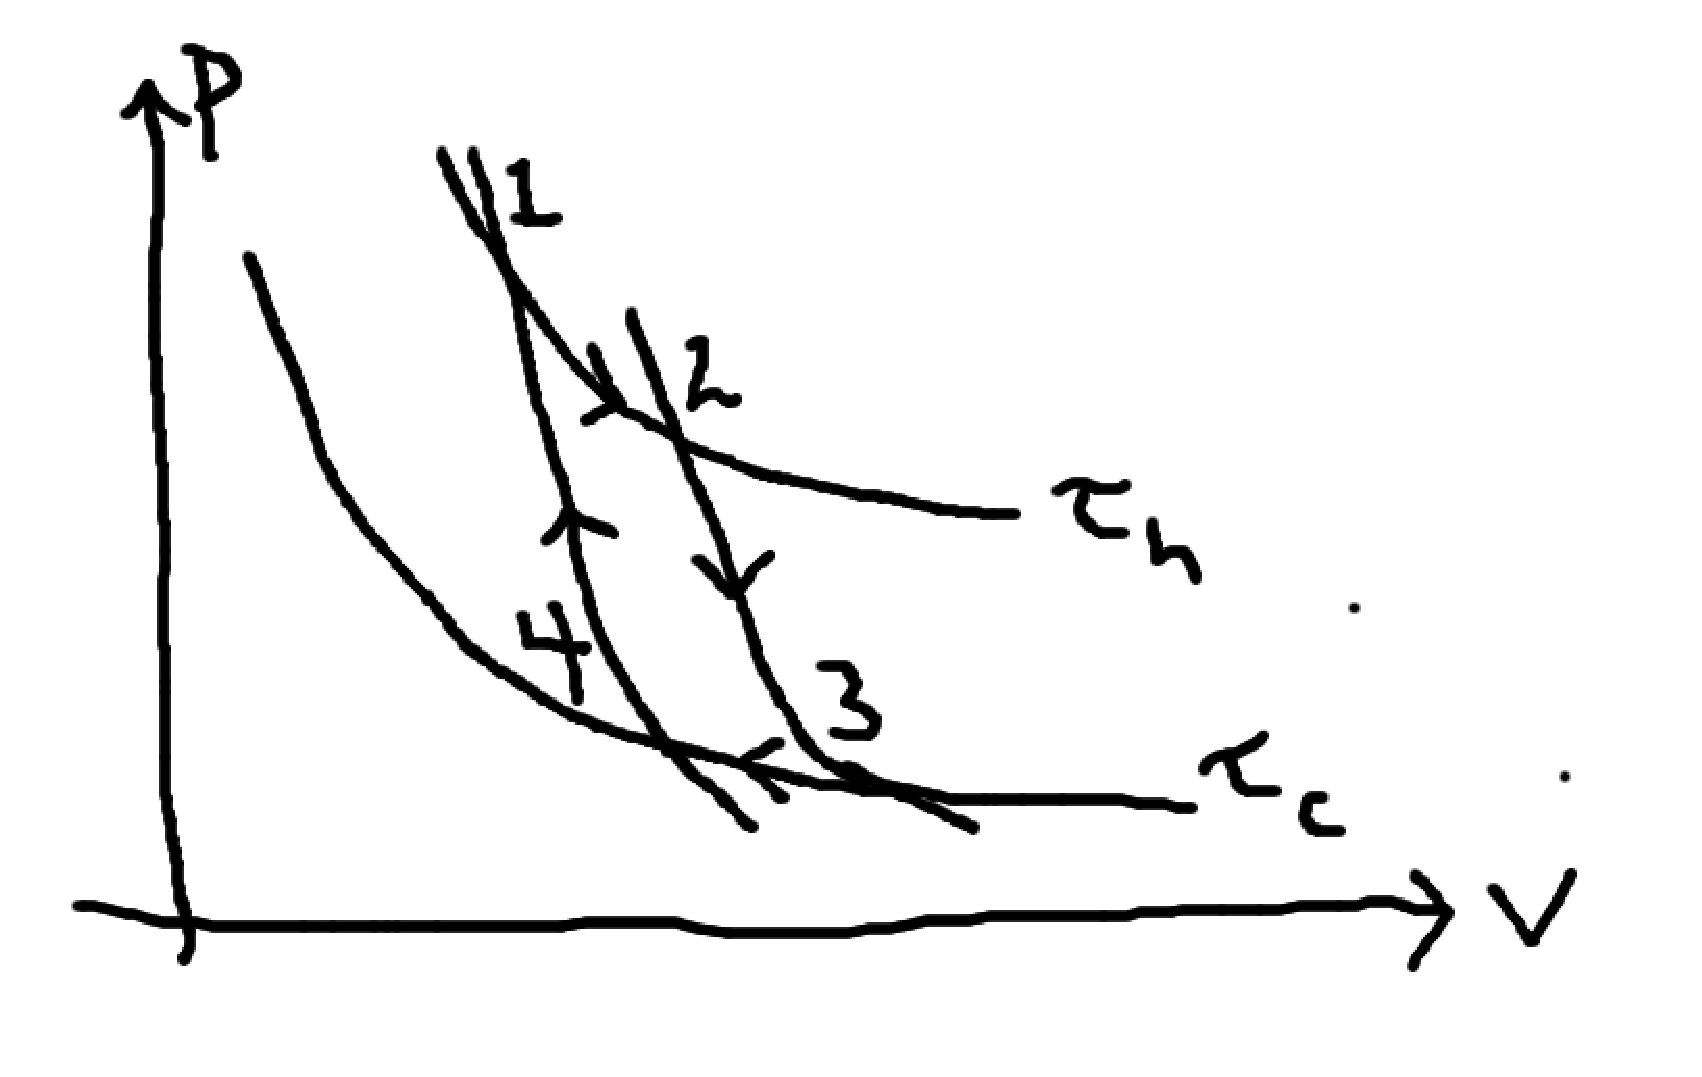
\includegraphics[height=5cm]{ambsthermopict/carnotengine.eps} 
} 
\caption{Carnot heat engine cycle.}
\label{carnotheatengine} 
\end{figure}  


\section{Classical Efficiency of a Carnot Heat Engine}

We now recall the classical analyis showing that 
the efficiency of a Carnot heat engine is
$1-\frac{\tau_c}{\tau_h}$. It is based on energy balance
in the form $dQ=d\tau +pdV=dE+dW$, where $dQ$ is supplied heat energy,
$d\tau$ change of internal energy, $dV$ change of volume $V$
and $dW$ change of work $W$.
We note that in process 12 and 23 work is done \emph{by} the process 
($dV>0$) and in step 34 and 41 \emph{on} the process ($dV<0$). 
Noting that $dQ=0$ in process 23 and 41, we obtain integrating
$d\tau +pdV=0$, 
\[
W_{23}=\int_2^3pdV=\tau_h-\tau_c=-\int_4^1pdV=-W_{41},
\]
where $W_{ij}$ is the work in process ij.
Further, recalling the state equation of a perfect gas
 $pV=(\gamma -1)\tau$, we get
integrating $0=\frac{d\tau}{\tau}+(\gamma -1)\frac{dV}{V}$ over
the processes 23 and 41,
\begin{equation}\label{logV}
(\gamma -1)\log(\frac{V_3}{V_2})=-\log(\frac{\tau_c}{\tau_h})
=-(\gamma -1)\log(\frac{V_1}{V_4}),
\end{equation}
where $V_i$ is the volume of state $i$.
Further, since $d\tau =0$ in process 12 and 34 
\[
W_{12}=Q_{12}, \quad W_{34}=Q_{34},
\]
where $Q_{ij}$ is the heat energy absorbed/released in process $ij$.
Using that $p=(\gamma -1)\tau_h/V$ in process 12, we have
\[
W_{12}=\int_1^2 pdv=(\gamma -1)\tau_h\int_1^2 \frac{dV}{V}=
(\gamma -1)\tau_h\log(\frac{V_2}{V_1}),
\]
and similarly
\[
W_{34}=(\gamma -1)\tau_c\log(\frac{V_4}{V_3}).
\]
We conclude since by (\ref{logV}), $\log(\frac{V_2}{V_1})=\log(\frac{V_3}{V_4})$\[
\frac{-W_{34}}{W_{12}}=\frac{\tau_c}{\tau_h}.
\]
Thus the efficiency $\eta_e$ of a Carnot heat engine, 
the quotient of performed work and used energy,
is given by
\[
\eta_e =\frac{W_{12}+W_{23}+W_{34}+W_{41}}{Q_{12}}=\frac{W_{12}+W_{34}}{W_{12}}=1-\frac{\tau_c}{\tau_h},
\]
as announced. The argument is based on an energy balance 
in the form $0=d\tau +pdV=d\tau +dW$ in the adiabatic
processes 23 and 34, and in the form $dQ=dW$
in the isothermal processes 12 and 34. Apparently we
have assumed that there is no loss in any these processes:
A Carnot engine is a heat engine without losses.   

In a realization of the above cyclic process 1-4 the flow
will be partly turbulent, in which case 
both $W_{12}>0$ and $W_{34}<0$
can only decrease. It follows that no heat engine
based on the cyclic process 1-4 can be more efficient than
a Carnot engine. A Carnot engine is really the best heat engine of the
form 1-4. But of course, the real issue is the efficiency of a real
heat engine, to which we return below. 



 
\chapter{Carnot Heat Pump}

\small
\begin{quote}
No heat pump can be more efficient than a 
Carnot heat pump with efficiency
$\tau_h/(\tau_h-\tau_c)$ operating between two temperatures 
$\tau_h$ and $\tau_c<\tau_h$.
(Carnot)
\end{quote}
\normalsize



\section{Classical Efficiency of a Carnot Heat Pump}

Running a Carnot heat engine in reverse, we get a \emph{Carnot
heat pump} absorbing energy
from a heat recervoir at low temperature and delivering 
heat energy to a recervoir at higher temperature $\tau_h>\tau_c$ at the expense of mechanical work, consisting of the following 
processes:
\begin{itemize}

\item[(21)] isothermal compression delivering heat energy at $\tau_h$
to a recervoir,
\item[(14)] adiabatic expansion to temperature $\tau_c$,
\item[(43)] isothermal expansion absorbing heat energy  
at $\tau_c$ from a recervoir,
\item[(32)] adiabatic compression to temperature $\tau_h$,
\end{itemize}
where now in step 21 and 32 work is done on the process and the work
in step 32 and 14 as above sums to zero.
The efficiency $\eta_p$ of Carnot heat pump is commonly measured by
the quotient of delivered heat energy $-Q_{21}$ divided by the 
total work $W$ supplied 
\begin{equation}\label{efficiencypump}
\eta_{p} =\frac{-Q_{21}}{W}=\frac{Q_{12}}{W}=\frac{1}{\eta_{e}}.
\end{equation}
A Carnot heat pump is an ideal heat pump without losses, 
while in a real heat pump 
the inevitable turbulence/shocks in the expansion steps 14 and 43 
would increase the temperature and thus reduce the heat absorption 
in step 43, thus reducing $Q_{43}$ and then also $-Q_{21}$ and 
the efficiency. 

Carnot's analysis captured in (\ref{efficiencypump}) suggests that
a lousy heat engine would be an excellent heat pump (and vice versa).
Of course, reality does not work this way, because of the inevitable
losses from turbulence.
Thus, Carnot's analysis at best only gives a very rough idea
of the efficiency of a heat engine or heat pump. 
We observe the obvious fact 
that even if the efficiency of a Carnot heat pump working with a
small temperature drop would seem to be formidable according
to classical analysis, it would 
tend to give a small output $-Q_{12}$ in absolute terms.

\begin{figure}[bhpt] 
\centerline{ 
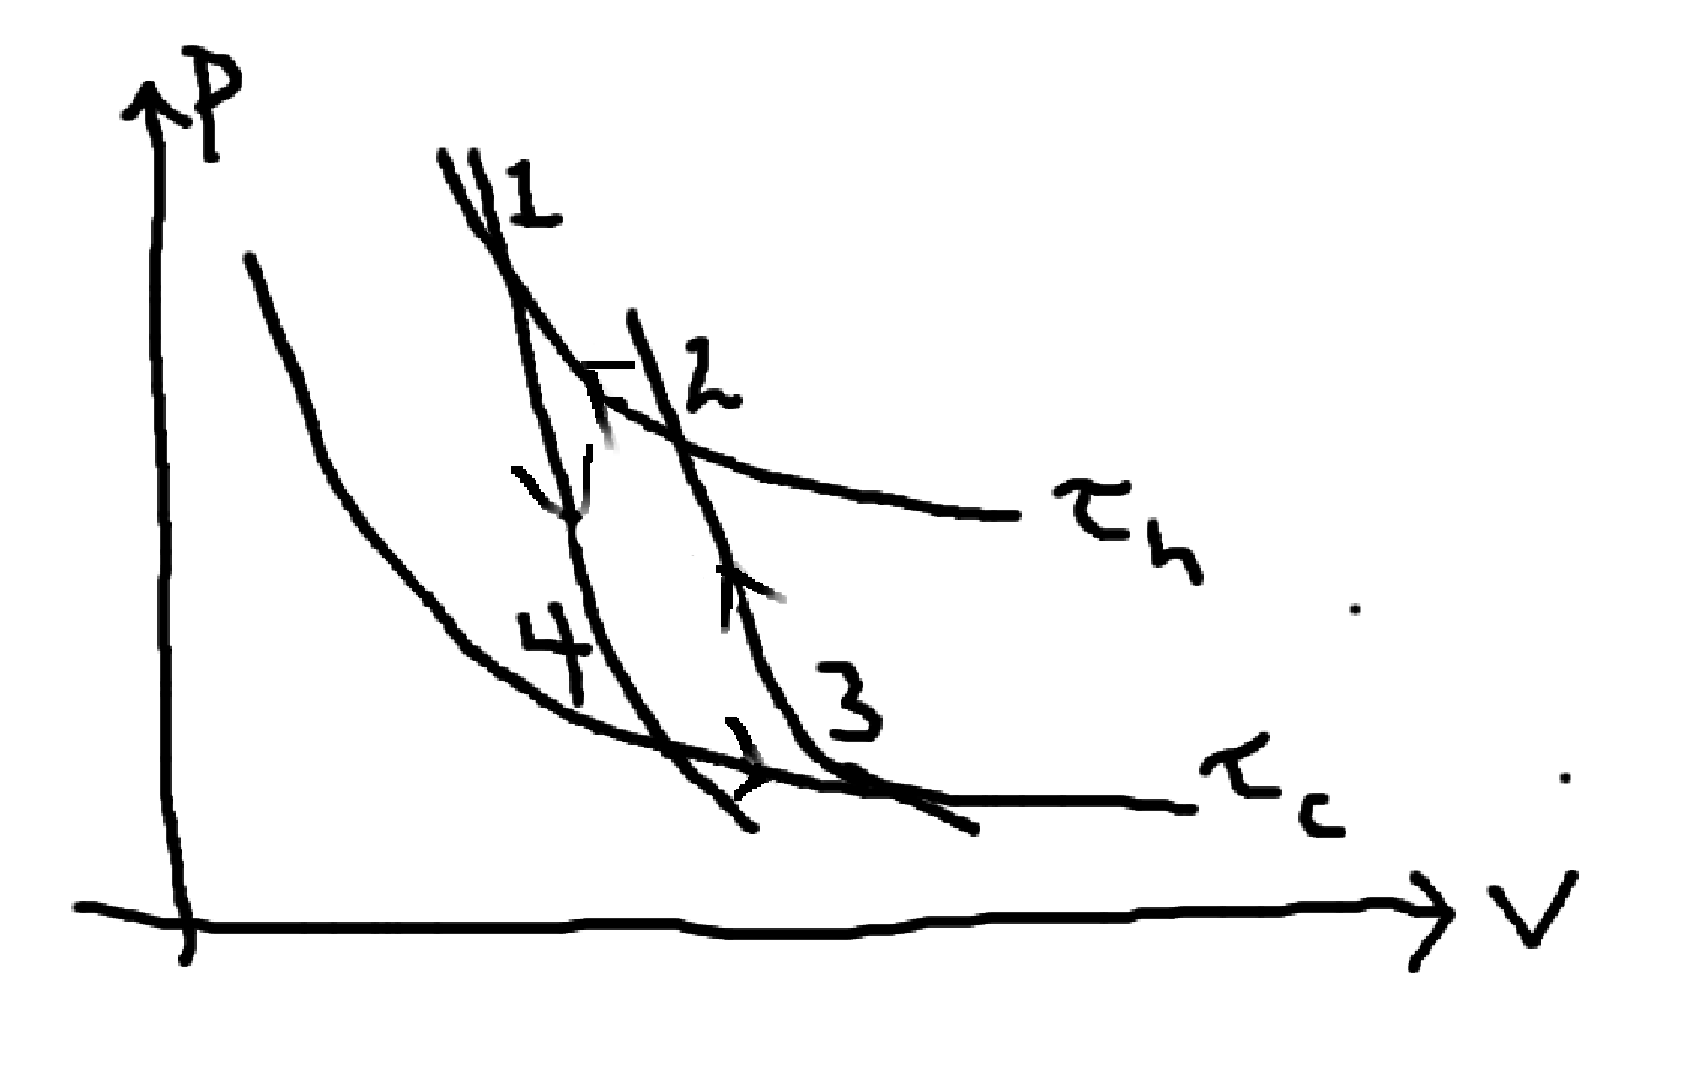
\includegraphics[height=5cm]{ambsthermopict/carnotpump.eps} 
} 
\caption{Carnot heat pump.}
\label{carnotheatpump} 
\end{figure}  

   
\chapter{Real Heat Engines}


\section{RNS Model of Real Heat Engine}

We simulate by RNS a real heat engine operating
through the same cycle of steps as the Carnot heat engine. 
We find that each step involves a certain loss due 
to turbulence/shocks and the total loss determines the
efficiency as compared to a Carnot engine.






\begin{figure}[bhpt] 
\centerline{ 
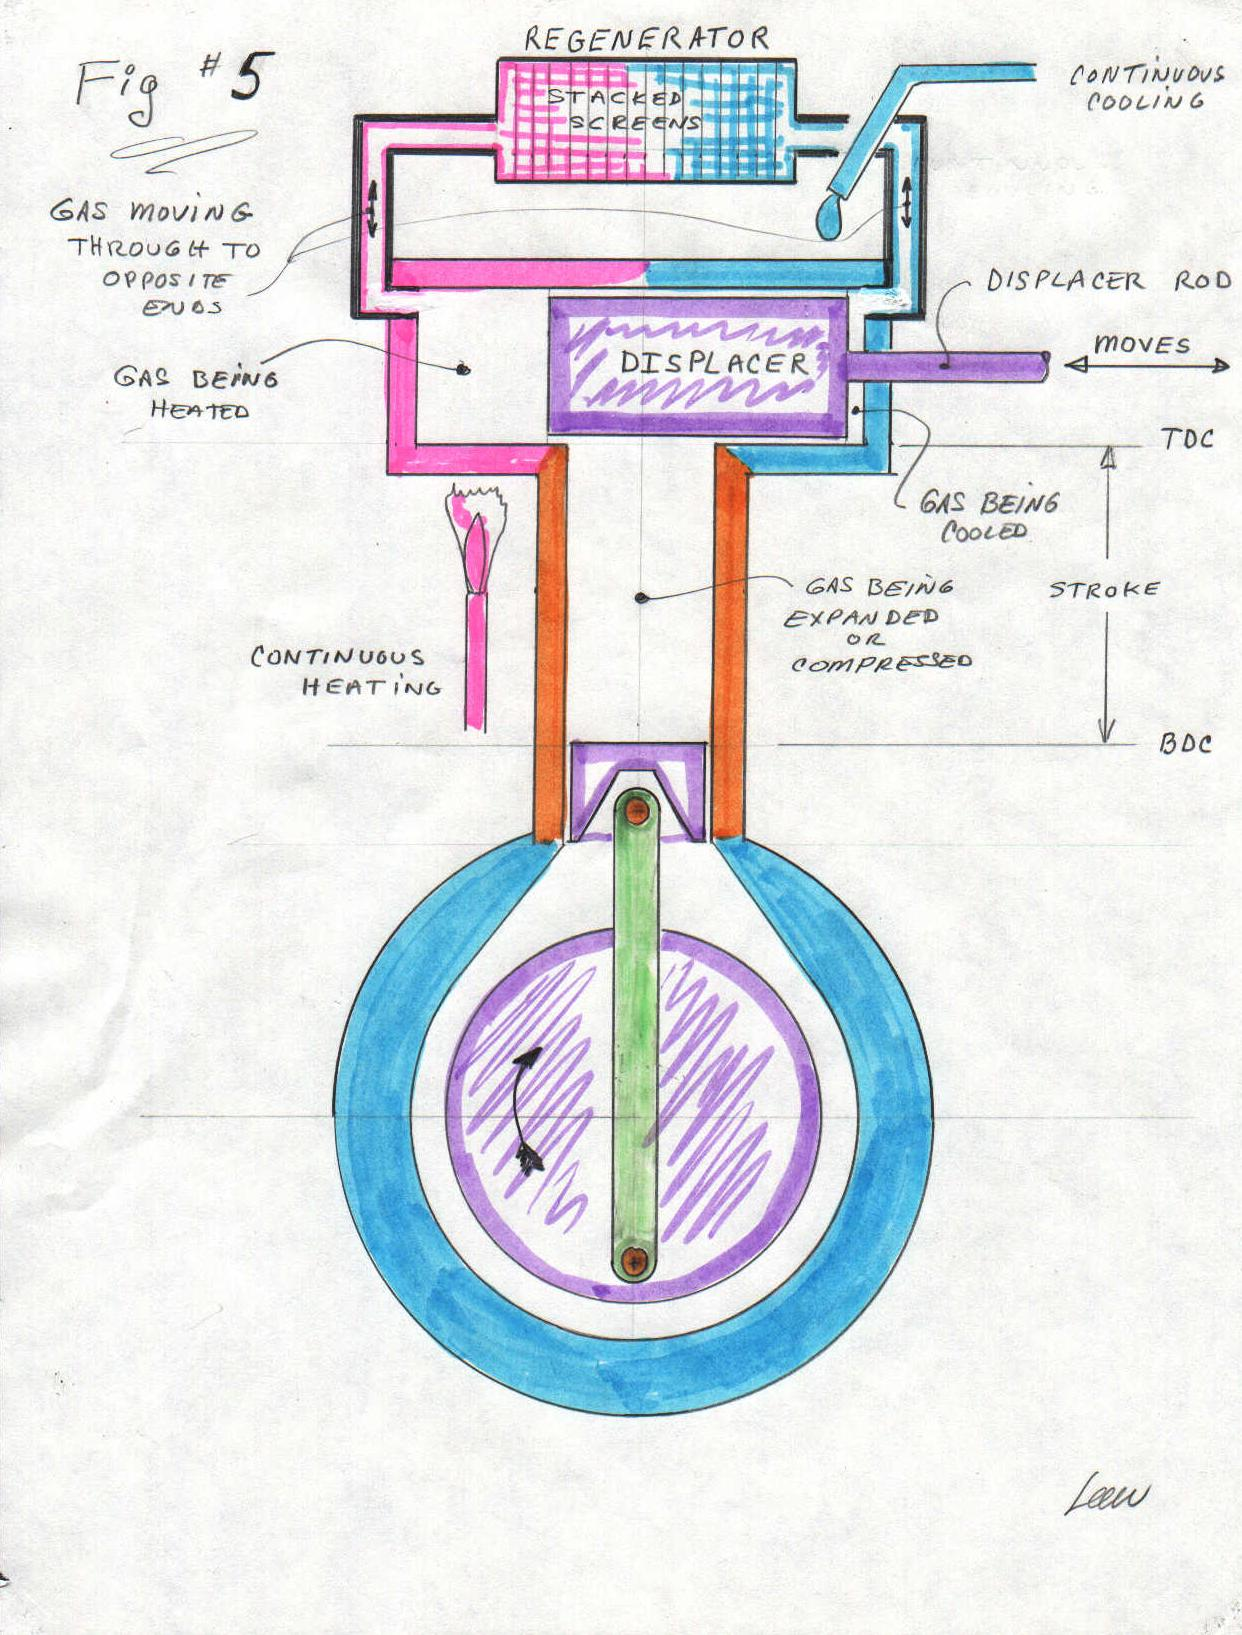
\includegraphics[height=12cm]{ambsthermopict/heatengine.eps} 
} 
\caption{A heat engine prototype}
\label{heatengineprototype} 
\end{figure}
  
\chapter{Real Heat Pumps}

\section{Increasing Efficiency by Phase Transition}

To increase the efficiency of a heat pump, the cycle
may be formed to contain a \emph{changes of phase} from fluid
to gas phase (\emph{evaporation}) in the expansion step  43 
and from ghas phase  
to fluid phase (\emph{condensation}) in step 21. The 
\emph{latent heat} being released during condensation and absorbed 
during the vaporization increase
both $Q_{43}$ and $-Q_{21}$ without increasing $W$, and thus
increases efficiency.

\begin{figure}[bhpt] 
\centerline{ 
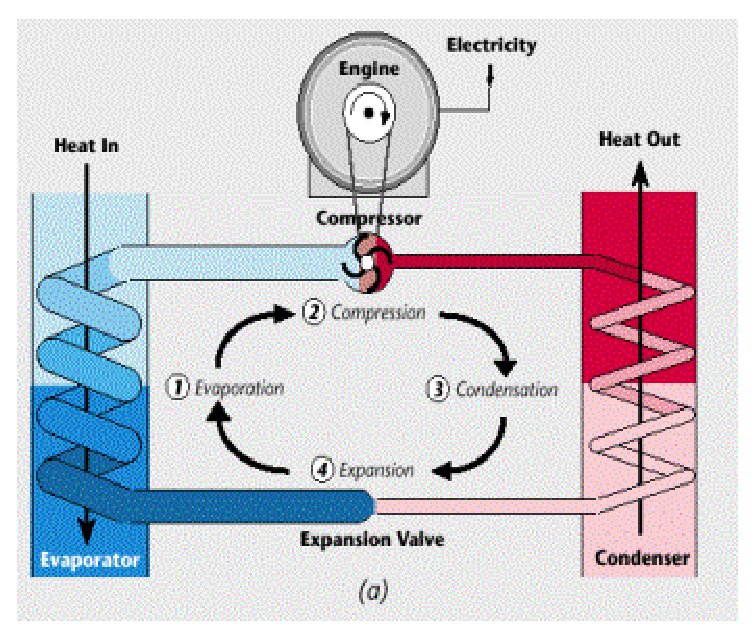
\includegraphics[height=8cm]{ambsthermopict/heat_pump.eps} 
} 
\caption{Principle of a  heat pump.}
\label{heatpump} 
\end{figure} 


\section{RNS Model of Real Heat Pump}

We simulate a simple heat pump consisting of two chambers 1  and 2
connected with a channel as in Joule's experiment. We assume the fluid 
moves back and forth between the two chambers being
in liquid phase in chamber 1 at pressure $p>p_c$ and in
gas phase in chamber 2 at pressure $p<p_c$, with $p_c$ the 
condensation/vaporization pressure, in the following cyclic process:


\begin{enumerate}
\item Open the valve in the channel and let the fluid at 
temperature $T_h$ and pressure $p>p_c$ in chamber 1 expand into
chamber 2 while evaporating into the gas phase at pressure
$p<p_c$ under temperture drop 
below $T_c$ in chamber 2. Close the valve.
\item Let chamber 2 absorb heat from a surrounding reservoir
at temperature $T_c$.
\item Open the valve and start a compressor in the channel
forcing the gas to move from chamber 2 into chamber 1, while
changing to fluid phase under release of heat, to reach 
a temperture above $T_h$ in chamber 1. Close the valve and stop the compressor.
\item Let the chamber 2 supply heat to a surrounding reservoir
at temperture $T_h$, and go back to 1.
\end{enumerate}
The heat consumed for evaporation and heat released by condensation
is modeled by defining the internal energy $e$ to be 
\begin{equation}\label{heatofformation}
e=\rho (T\pm \Delta H)
\end{equation}
where $\Delta H$ is a constant heat of formation, 
or change of enthalpy $H$, the plus-sign is
used if $p>p_c$, the minus-sign if $p<p_c$, and $p_c$ is the
pressure at which condensation and evaporation takes place.
For simplicity we assume that $p_c$ does not depend on temperature. 

We model the cyclic process by the one-fluid compressible Euler equations
with internal energy given by (\ref{heatofformation}), the heat
release in chamber 2 and the heat absorbtion in chamber 2 by 
suitable source terms in the energy equation, and the compression
in the channel by a volume force in the momentum equation.
We compute the efficiency $\eta_p$ as defined above.

\chapter{Refrigerators}

\small
\begin{quote} The final aim of all science is to resolve itself
into mechanics. (Helmholtz)
\end{quote}
\begin{quote} The orbit of the electron obeys no law....All is caprice,
the calculable world has become incalculable....superstitions have
risen from the dead and cast down the mighty from their seats and put
paper crowns on presumptious fools. (Bernard Shaw in 
\emph{Too True to be Good})
\end{quote}
\normalsize

\section{Importance of Cooling}

Without refrigerators, modern society and urban life, would be
very complicated, if not impossible. The traditional method 
for storing food by cooling in countries with a Winter season, used
well into the middle of the 19th century,
was to store ice harvested in the Winter, typically
under thick layers of saw dust, to use it over the Summer season.
To cool a multi-million city this way would require enormous
installations. 

\section{The Compressor Refrigerator}

A refrigerator is a form of heat pump, absorbing heat energy from
a reservoir at low temperature (the inside of the refrigerator)
and delivering heat energy to a reservoir at higher 
temperature (to the surrounding
room). The above analysis directly applies and the maximal Carnot efficiency 
is given by
\begin{equation}\label{efficiencyref}
\eta_{r} =\frac{Q_{43}}{W}=\frac{1}{\eta_{e}}.
\end{equation}
A refrigerator would suffer losses in the expansion steps 14 and 43 
increasing the temperature and reducing the heat absorption 
in process  43, thus reducing $Q_{43}$ and the efficiency. 

A regular refrigerator uses a compressor for the condensation
from gas to fluid phase. A compressor is a mechanical device with
a rotating fan powered by electricity, which causes a certain noise.

\begin{figure}[bhpt] 
\centerline{ 
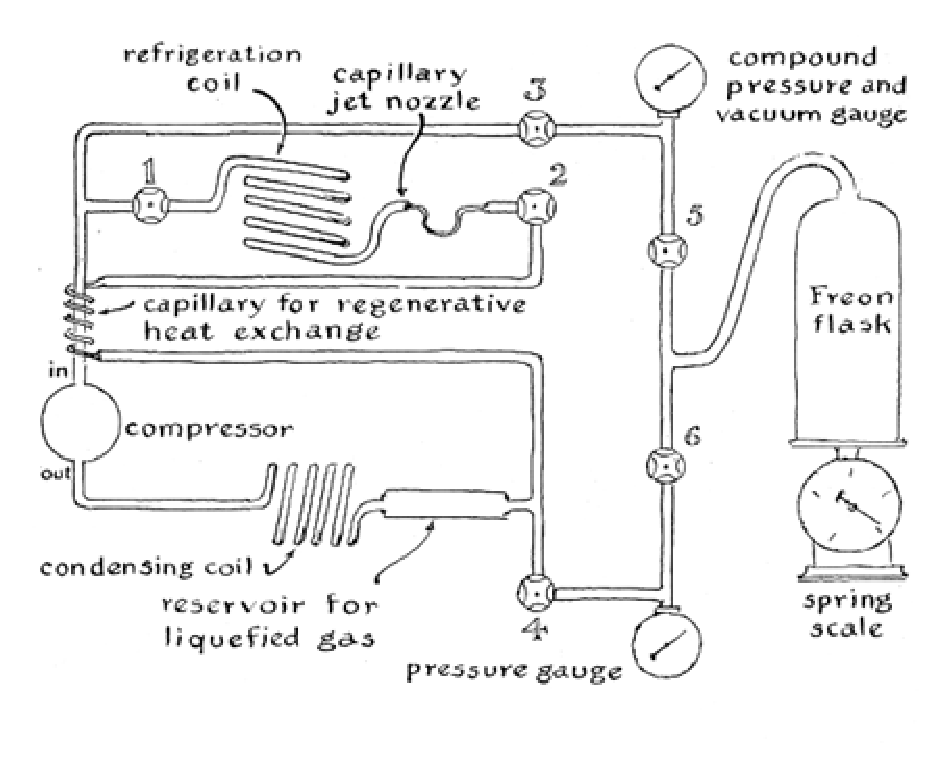
\includegraphics[height=8cm]{ambsthermopict/refrigeratorprin.eps} 
} 
\caption{Principle of a compressor refrigerator}
\label{refrigerator} 
\end{figure} 

\section{Absorption Refrigerator of Platen/Munters}

An absorption refrigerator uses a different 
method that requires no moving parts (thus reducing noise)
and is powered only by heat. By supplying heat you thus generate
cold, which is apparent contradiction with the 2nd Law in
Clausius form stating that heat can only ``spontaneously''go from hot
to cold.   
Typically, it uses three substances: ammonia, hydrogen 
gas, and water. Normally, ammonia is a gas at room temperature 
(with a boiling point of -33�C), but the system is pressurized to the 
point that the ammonia is a liquid at room temperature.

We cite from Wikipedia: \emph{The cooling cycle starts at the evaporator, where liquefied anhydrous 
ammonia enters. (Anhydrous means there is no water in the ammonia, which 
is critical for exploiting its sub-zero boiling point.) The "evaporator" 
contains another gas (in this case, hydrogen), whose presence lowers the 
partial pressure of the ammonia in that part of the system. The total 
pressure in the system is still the same, but now not all of the pressure 
is being exerted by ammonia, as much of it is due to the pressure of the 
hydrogen. Ammonia doesn't react with hydrogen - the hydrogen is there 
solely to take up space - creating a void that still has the same pressure 
as the rest of the system, but not in the form of ammonia. 
Per Dalton's law, the ammonia behaves only in response to the proportion 
of the pressure represented by the ammonia, as if there was a vacuum and 
the hydrogen wasn't there. Because a substance's boiling point changes with pressure, the lowered partial pressure of ammonia changes the ammonia's boiling point, bringing it low enough that it can now boil below room temperature, as though it wasn't under the pressure of the system in the first place. When it boils, it takes some heat away with it from the evaporator - which produces the "cold" desired in the refrigerator.}


\emph{The next step is getting the liquid ammonia back, as now it's a gas and mixed with hydrogen. Getting the hydrogen away is simple, and this is where the "absorber" comes in. Ammonia readily mixes with water, and hydrogen does not. The absorber is simply a downhill flow of tubes in which the mixture of gases flows in contact with water being dripped from above. Once the water reaches the bottom, it's thoroughly mixed with the ammonia, and the hydrogen stays still (though it can flow freely back to the evaporator).}


\emph{At this point, the ammonia is a liquid mixed with water and still not usable for refrigeration, as the mixture won't boil at a low enough temperature to be a worthwhile refrigerant. It's now necessary to separate the ammonia from the water. This is where the heat from the flame comes in. When the right amount of heat is applied to the mixture, the ammonia bubbles out. This phase is called the "generator". The ammonia isn't quite dry yet - the bubbles contain gas but they're made of water, so the pipe twists and turns and contains a few minor obstacles that pop the bubbles so the gas can move on. The water that results from the bubbles isn't bad - it takes care of another need, and that is the circulation of water through the previous absorption step. Because that water has risen a bit while it was bubbling upwards, the flow of that water falling back down due to gravity can be used for this purpose. The maze that makes the ammonia gas go one way and the bubble water go the other is called the "separator".}

\emph{The next step is the condenser. The condenser is a sort of heat sink or heat exchanger that cools the hot ammonia gas back down to room temperature. Because of the pressure and the purity of the gas (there is no hydrogen here), the ammonia condenses back into a liquid, and at that point, it's suitable as a refrigerant and the cycle starts over again.}


\emph{The absorption refrigerator was invented by Baltzar von Platen and Carl Munters in 1922, while they were still students at the Royal Institute of Technology in Stockholm, Sweden. Commercial production began in 1923 by the newly formed company AB Arctic, which was bought by Electrolux in 1925.}



\section{Simulation of Compressor Refrigerator}


%\chapter{Reactive Thermodynamics}

%\chapter{Combustion Engines}

%We study the efficiency of a simple combustion engine = reactive
%flow plus a moving piston.

\fi  % --- end removed block (Carnot Heat Engine, Carnot Heat Pump, Real Heat Engines, Real Heat Pumps, Refrigerators) ---

\iffalse  % --- moved to Part II right after Dual Linearized Problem (chapters/move_cosmology.tex) ---
\chapter{Cosmology: RNS with Gravitation}

\small
\begin{quote} According to the \emph{Perfect Cosmological Principle}, 
the Universe on a large scale looks the same everywhere and at all times.
(Fred Hoyle)
\end{quote}
\begin{quote} The thermodynamic properties of self-gravitating
systems are still unclear...The tendency of increasing granularity with time
(in a self-gravitating system), so important to the structure and development 
of the Universe, seems to represent a fundamental principle. 
(Paul Davies \cite{davies})
\end{quote}
\begin{quote} 
GRAVITATION: The universal property of all material objects
to attract each other.\\
GRAVITON: A hypothetical particle which, when passing
to and fro in virtual form bewteen two masses, in large numbers,
is thought to mediate the gravitational attraction between them.
(Guillemin \cite{guillemin})
\end{quote}
\normalsize

\normalsize

\section{Euler's Equations with Gravitation}

The Euler equations including gravitational forces from the mass distribution
can be viewed as a basic (non-relativistic) \emph{cosmological model}.  
We thus consider an inviscid perfect gas 
enclosed in a volume $\Omega$ in $\bbR^3$ with boundary $\Gamma$
(or the whole of $\bbR^3$), over a time interval $I=(0,1]$, assuming 
that the gas is subject to a gravitational force $\nabla\varphi$, where
$\varphi$ is a \emph{gravitational potential} 
coupled (at each time instant) to the mass distribution $\rho$  
through Poisson's equation $\Delta\varphi =\rho$
with (for simplicity) $\varphi =0$ on $\Gamma$. This is a 
\emph{self-gravitating system} since the gravitational force depends
on the mass-distribution  

Replacing $\rho$ by $\Delta\varphi$, we are led to the following version
of Euler's equations with gravitation:  
Find $\hat u=(\varphi ,m,e)$ 
depending on $(x,t)\in Q\equiv \Omega\times I$ such that
\begin{equation}\label{eulergrav}
\begin{array}{rcl}
\Delta\dot\varphi +\nabla\cdot m &=&  0 \quad \mbox{in } Q, \\
\dot m +\nabla\cdot (mu) +\nabla p-\rho\nabla\varphi&=&  0 \quad \mbox{in } Q, \\
\dot e +\nabla\cdot (eu)+p\nabla\cdot u &=& 0  \quad \mbox{in } Q,\\ 
u\cdot n&=&0\quad \mbox{on } \Gamma\times I\\
\varphi &=&0\quad \mbox{on } \Gamma\times I\\
\hat u(\cdot ,0)&=&\hat u^0\quad \mbox{in } \Omega , 
\end{array} 
\end{equation}
where $u=\frac{m}{\Delta\varphi}$, 
$p=(\gamma -1)e$ with $\gamma >1$, and we normalize the gravitational
constant to unity.

\section{The Hen and the Egg}

An interesting aspect of this model with the gravitational
potential $\varphi$ as a primary variable and the mass distribution
$\rho$ as a derived quantity, is that it does not include
\emph{action at distance} in the same way as the conventional model
with $\varphi$ derived from $\rho$ through Poisson's equation 
$\Delta\varphi =\rho$. Instead we have to deal
with the new equation $\Delta\dot\varphi +\nabla\cdot m =0$,
still containing the Laplacian.

Considering the equation $\Delta\varphi =\rho$ as defining
$\varphi$ in terms of $\rho$ or vice versa, of course connects
to which comes first: the egg or the hen. 

Choosing (in an exam for example) 
to explain either how a hen can lay an egg
or how an egg can develop into a hen, you may go for the first
option as appearing to be (somewhat) simpler to deal with.
The idea would be that it would be advantageous to
choose the more complex object of the 
potential/hen rather than the simpler mass/egg, as 
the primary unknown which will come out by solving the equations,
(by some form of computation).
Thus the more complex object, the potential/hen will 
be ``created by computation'' in front of our eyes, thus relieving us
from \emph{explaining} how a mass/egg can create a potential/hen. 
But doing so we have to deal with 
the equation $\Delta\dot\varphi +\nabla\cdot m=0$
expressing ``mass conservation'' in a non-standard form,
which  admittedly seems to involve action at distance if we rewrite it in the form.
$\dot\varphi +(\Delta )^{-1}\nabla\cdot m=0$ for the purpose
of explicitly updating $\varphi$ by time-stepping. What can we do 
to allow time-stepping without inverting the Laplacian?

\section{Perturbed Mass Conservation} 

Well, we may consider
to perturb the equation for mass conservation
$\Delta\dot\varphi +\nabla\cdot m=0$ into: 
\[
\kappa\ddot\varphi -  \Delta\dot\varphi -\nabla\cdot m=0
\]
with $\kappa$ a small positive constant, now allowing time stepping
without inverting the Laplacian. Of course, you could regularize the
equation $\Delta\varphi =\rho$ similarly into  
$\kappa\dot\varphi -\Delta\varphi =\rho$ keeping mass conservation in the
standard form $\dot\rho +\nabla\cdot (\rho u)=0$. In any case,
(\ref{eulergrav}) with $\varphi$ instead of $\rho$ and a perturbed
equation for mass conservation, is a model without action at distance.


\section{Gravitons?}

Solving Poisson's equation $\Delta\varphi =\rho$
equation for the gravitational
potential $\varphi$ in terms of the density $\rho$, reflect that
(somehow) a mass distribution ``creates'' its own gravitational field
(seemingly infinitely fast). The physics of this creation of a hen out
of an egg in the form of
a gravitational potential/force from a mass distribution, is unknown: A
conjecture is that the gravitational field is 
established through an \emph{exchange} of certain hypothetical particles 
called \emph{``gravitons''}. But no gravitons have been detected despite
intense search.



The reverse question is how a hen can lay an egg 
or how a gravitational potential can ``create'' a mass.
A potential with a sharp peak of the form 
$\frac{1}{4\pi\vert x-\bar x\vert}$, would then represent a
unit mass at position $\bar x$.  
In this perspective a tendency of ``mass lumping'' from 
very small initial density
variations, is to be expected from the fact that application of the Laplacian
may enhances variations and thus create positive and negative peaks/masses
out of nothing, with masses of different equal signs attracting each other
and masses with different signs repelleing each other. Our Universe
with positive masses would thus have a twin Universe with negative masses.

In this model, it is thus the gravitational 
potential $\phi$, which is given initially
and which evolves in time (together with momentum and energy)
and from which the mass density $\rho$ is generated by $\Delta\phi =\rho$
in a local ``creation process''.
We here avoid action at distance and we also get a hint
to the possible nature of all the ``dark mass'' seemingly required to account 
for the observed gravitational forces on cosmic scales, as 
mollified potential peaks not strong enough to 
``create visible mass'', but yet having gradients and exerting
gravitational forces.

%The alternative model (\ref{cosmology2}) with $\delta >0$ is a wave equation 
%with finite speed of propagation depending on $\delta$. The proper choice
%of $\delta$ from physical point of view is unclear, while 
%we expect certain outputs to be insensitive to the choice of $\delta$.

\section{The 2nd Law with Gravitation}

The 2nd Law with gravitation takes the form
\begin{equation}
\dot K=W-D+ P,\quad \dot E=-W+D,\quad D>0,
\end{equation}
where 
\[
\begin{split}
P&=-\int_\Omega \rho\nabla\varphi\cdot u\, dx =+\int_\Omega \varphi\nabla\cdot m\, dx=-\int_\Omega\varphi\dot\rho\, dx= \dot\Phi,\\
\Phi &=-\frac{1}{2}\int_\Omega \varphi\Delta\varphi\,dx =\frac{1}{2}\int_\Omega\vert\nabla\varphi\vert^2\, dx.
\end{split}
\] 
By summation, we have
\[
\frac{d}{dt}(K+E -\Phi)=0
\]
stating that the total energy, the sum of
kinetic, heat and gravitational energy $K+E -\Phi$, is conserved.

\section{Irreversibility and Heat Death}

A natural scenario is to start with a hot compressed gas at rest, which is
let free to expand in a \emph{Big Bang} with $W-D-P>0$ setting the
gas in motion until $W-D-P<0$ and $K=0$, whereupon the gas
contracts by gravitation back to a hot compressed state in a \emph{Big Crunch}
allowing the process to start all over with a new Big Bang.

In each cycle of this process some kinetic energy would irreversibly
be transformed into heat energy, which ultimately could lead to 
a stationary state with $W=D$ and $P=0$, a \emph{heat death}. But the 
whole process may have many cycles....and so there may have been Worlds
and intelligent cultures including thermodynamics  
even before the Big Bang of the World we happen to live in...   

\section{A Self-Gravitating Gas in a Box}

To probe the thermodynamics of (\ref{eulergrav}) concretely we solve a
discrete form on a cubic grid filling a box $\Omega =[0,1]^3$, in conservation
form for the density $\rho$, the momentum $m=\rho u$ and the internal energy
density $e$, with the ideal-gas closure
\begin{equation}\label{closure}
p=(\gamma -1)e=\rho T,\qquad \gamma >1,
\end{equation}
so that $T=p/\rho$ is the temperature and $\gamma$ the adiabatic index. The
self-gravitation is supplied through the \emph{mean-subtracted} Poisson coupling
\begin{equation}\label{jeansswindle}
\Delta\varphi = G\,(\rho -\bar\rho ),\qquad
\bar\rho =\frac{1}{\vert\Omega\vert}\int_\Omega\rho\, dx,
\end{equation}
with $\varphi =0$ on $\Gamma$, where $G>0$ is the \emph{gravitational coupling}
(playing the role of $4\pi G_{\mathrm{Newton}}$) and $\bar\rho$ the mean density.

The subtraction of $\bar\rho$ is essential and is the classical
\emph{Jeans swindle}. A strictly uniform gas in a \emph{finite} box is not
force-free if $\rho$ itself sources $\varphi$: with $\varphi =0$ on $\Gamma$ the
solution of $\Delta\varphi =G\rho$ bulges in the interior, so a net inward force
develops everywhere and the whole box \emph{breathes} in and out --- an artifact
of the boundary rather than of any structure in the gas. Sourcing $\varphi$ from
the density \emph{contrast} $\rho -\bar\rho$ makes the uniform background exactly
force-free, so that only departures from uniformity gravitate. This is precisely
what one wants of a cosmological model: it is the \emph{granularity}, not the
mean, that drives the dynamics.

The model so written has exactly \emph{two} control parameters: the
gravitational coupling $G$ and the adiabatic index $\gamma$. Everything in the
competition between collapse and dispersal is decided by these two, as we now
show.

\section{Pressure versus Gravitation: the Jeans Criterion}

Linearize (\ref{eulergrav}), (\ref{closure}), (\ref{jeansswindle}) about a
uniform state $\rho =\bar\rho$, $u=0$, $T=\bar T$ at rest. Writing the density
perturbation as $\delta\rho$ and eliminating $m$ and $\varphi$ one obtains the
wave equation
\begin{equation}\label{waveeq}
\ddot{\delta\rho}=c_s^2\,\Delta(\delta\rho)+G\bar\rho\,\delta\rho,
\qquad c_s^2=\gamma\,\frac{\bar p}{\bar\rho}=\gamma\bar T,
\end{equation}
where $c_s$ is the adiabatic sound speed. For a plane wave
$\delta\rho\propto\exp(i(k\cdot x-\omega t))$ this gives the
\emph{Jeans dispersion relation}
\begin{equation}\label{dispersion}
\omega^2=c_s^2k^2-G\bar\rho=\gamma\bar T\,k^2-G\bar\rho .
\end{equation}
The first term, from pressure, is \emph{stabilizing} (it grows with $\gamma$);
the second, from gravitation, is \emph{destabilizing} (it grows with $G$). A
perturbation grows --- the gas \emph{collapses} --- precisely when
$\omega^2<0$, i.e.\ when
\begin{equation}\label{jeanscrit}
G\bar\rho>\gamma\bar T\,k^2
\qquad\Longleftrightarrow\qquad
\lambda>\lambda_J=2\pi\sqrt{\frac{\gamma\bar T}{G\bar\rho}}\, ,
\end{equation}
$\lambda_J$ being the \emph{Jeans length}. Below the Jeans length pressure wins
and the perturbation merely oscillates as a sound wave ($\omega^2>0$); above it
gravity wins and the perturbation grows.

The decisive observation is that the onset of collapse depends on $G$ and
$\gamma$ \emph{only through the ratio} $G/\gamma$: at a fixed scale $k$ and
fixed background $(\bar\rho ,\bar T)$, doubling the coupling $G$ has exactly the
same effect as halving the stiffness $\gamma$. The dimensionless number that
decides everything is
\begin{equation}\label{jeansnumber}
J=\frac{G\bar\rho}{\gamma\bar T\,k^2},
\qquad\text{collapse}\iff J>1 .
\end{equation}

In a box of side $L$ the longest available wavelength is $\lambda\approx L$, so
structure forms \emph{at all} only if $\lambda_J\lesssim L$, that is
\begin{equation}\label{boxthreshold}
G\gtrsim (2\pi)^2\,\frac{\gamma\bar T}{\bar\rho\,L^2}.
\end{equation}
For $\gamma =2$ and $\bar T=\bar\rho =L=1$ this requires $G\gtrsim 79$; for a
seed of size $\sim L/3$ the threshold is about nine times larger. Below it the
box is Jeans-stable at \emph{every} scale and any initial lump simply pulsates.
This is why a modest coupling produces only an oscillation and never a collapse:
$G$ has not been pushed past the Jeans threshold set by $\gamma$.

\section{Collapse to a Stable Configuration: the Role of $\gamma$}

The Jeans criterion (\ref{jeanscrit}) decides whether collapse \emph{begins}.
Whether the collapse \emph{ends} in a stable, finite lump --- rather than
running away to a singular spike --- is a separate question, and it is decided
by $\gamma$ \emph{alone}, independently of $G$.

Consider a self-gravitating polytropic cloud of fixed mass $M$ and radius $R$.
Under adiabatic compression $p\propto\rho^\gamma$, so the internal energy
density scales as $e\propto\rho^\gamma\propto R^{-3\gamma}$ and the total
internal (thermal) energy as
\[
U=\int_\Omega e\,dx \;\propto\; R^{-3\gamma}\cdot R^3 \;=\; R^{-3(\gamma -1)},
\]
while the gravitational self-energy scales as
\[
W \;\propto\; -\frac{GM^2}{R}\;\propto\; -R^{-1}.
\]
The total energy is therefore $E(R)=A\,R^{-3(\gamma -1)}-B\,R^{-1}$ with
$A,B>0$. As $R\to 0$ the thermal term dominates --- and hence $E$ possesses a
\emph{minimum} at a finite radius, a stable hydrostatic equilibrium --- if and
only if it stiffens faster than gravity, $3(\gamma -1)>1$, that is
\begin{equation}\label{fourthirds}
\boxed{\;\gamma>\tfrac43\;}
\end{equation}
the classical \emph{Chandrasekhar index}. The three regimes are:
\begin{itemize}
\item $\gamma>\tfrac43$: pressure wins under compression; collapse is
\emph{arrested} at a finite quiescent lump, possibly after damped oscillations.
\item $\gamma<\tfrac43$: gravity wins at every compression; collapse
\emph{runs away}, no equilibrium exists.
\item $\gamma=\tfrac43$: the marginal case (governing, e.g., white-dwarf
stability).
\end{itemize}
Thus the two parameters play complementary roles: $G$ (through (\ref{jeanscrit}))
selects \emph{which scales collapse and how fast}, while $\gamma$ (through
(\ref{fourthirds})) decides \emph{whether the collapse can be stopped}. To reach
a stable bound configuration one needs \emph{both} a coupling $G$ large enough
to cross the Jeans threshold \emph{and} a stiffness $\gamma>\tfrac43$ so that the
endpoint is an equilibrium rather than a singularity.

\section{Breathing, Sloshing and Virialization}

These two criteria account for the phenomenology seen in the simulations.

\emph{Breathing.} A uniform gas in which $\rho$ (rather than $\rho-\bar\rho$)
sources $\varphi$ is not in equilibrium in a finite box: it contracts toward the
centre, pressure builds, it rebounds, and the box breathes globally while its
density stays nearly uniform. The Jeans swindle (\ref{jeansswindle}) removes
this boundary artifact, leaving only the genuine gravitational response to
density contrast.

\emph{Sloshing.} A pair of overdensities below the Jeans threshold
($J<1$ at their separation) does not collapse but exchanges mass back and forth
quasi-periodically between the two centres. This is a \emph{virial oscillation}
in the double-well gravitational potential: gas falling toward one centre
overshoots on its pressure and inertia, sloshes to the other, and returns. With
$\gamma>\tfrac43$ and no dissipation the oscillation is undamped, kinetic and
gravitational energy being traded reversibly, $\dot K=P=\dot\Phi$, exactly as in
the energy balance of \S\,\textit{The 2nd Law with Gravitation}.

\emph{Virialization.} To settle into a quiescent lump the gas must \emph{shed}
its infall energy: a stable bound configuration requires dissipation $D>0$ to
convert the ordered kinetic energy of collapse into heat. The entropy so
produced is the irreversible price of structure formation --- the mechanism
behind Davies' ``increasing granularity'' (\S\,\textit{Cosmology}) and behind
the heat death of \S\,\textit{Irreversibility and Heat Death}. Gravitational
structure forms by the conversion, through $D$, of gravitational potential
energy first into bulk motion and then, irreversibly, into heat.

\begin{remark}
In the numerical model the closure is written as $p=\gamma_s\,e$, so that the
adiabatic index is $\gamma=1+\gamma_s$; the stability boundary (\ref{fourthirds})
then reads $\gamma_s>\tfrac13$, and the coupling $G$ is exactly the
$4\pi G_{\mathrm{Newton}}$ of (\ref{jeansswindle}). The two sliders $(G,\gamma_s)$
of the interactive model are precisely the two parameters $(G,\gamma)$ of the
analysis above.
\end{remark}

\section{RNS Simulations of a Self-Gravitating Gas}

We give below some results from RNS solutions of (\ref{eulergrav})
showing the development mass granularity from
uniform mass distributions under expansion.

\begin{figure}[bhpt] 
\centerline{ 
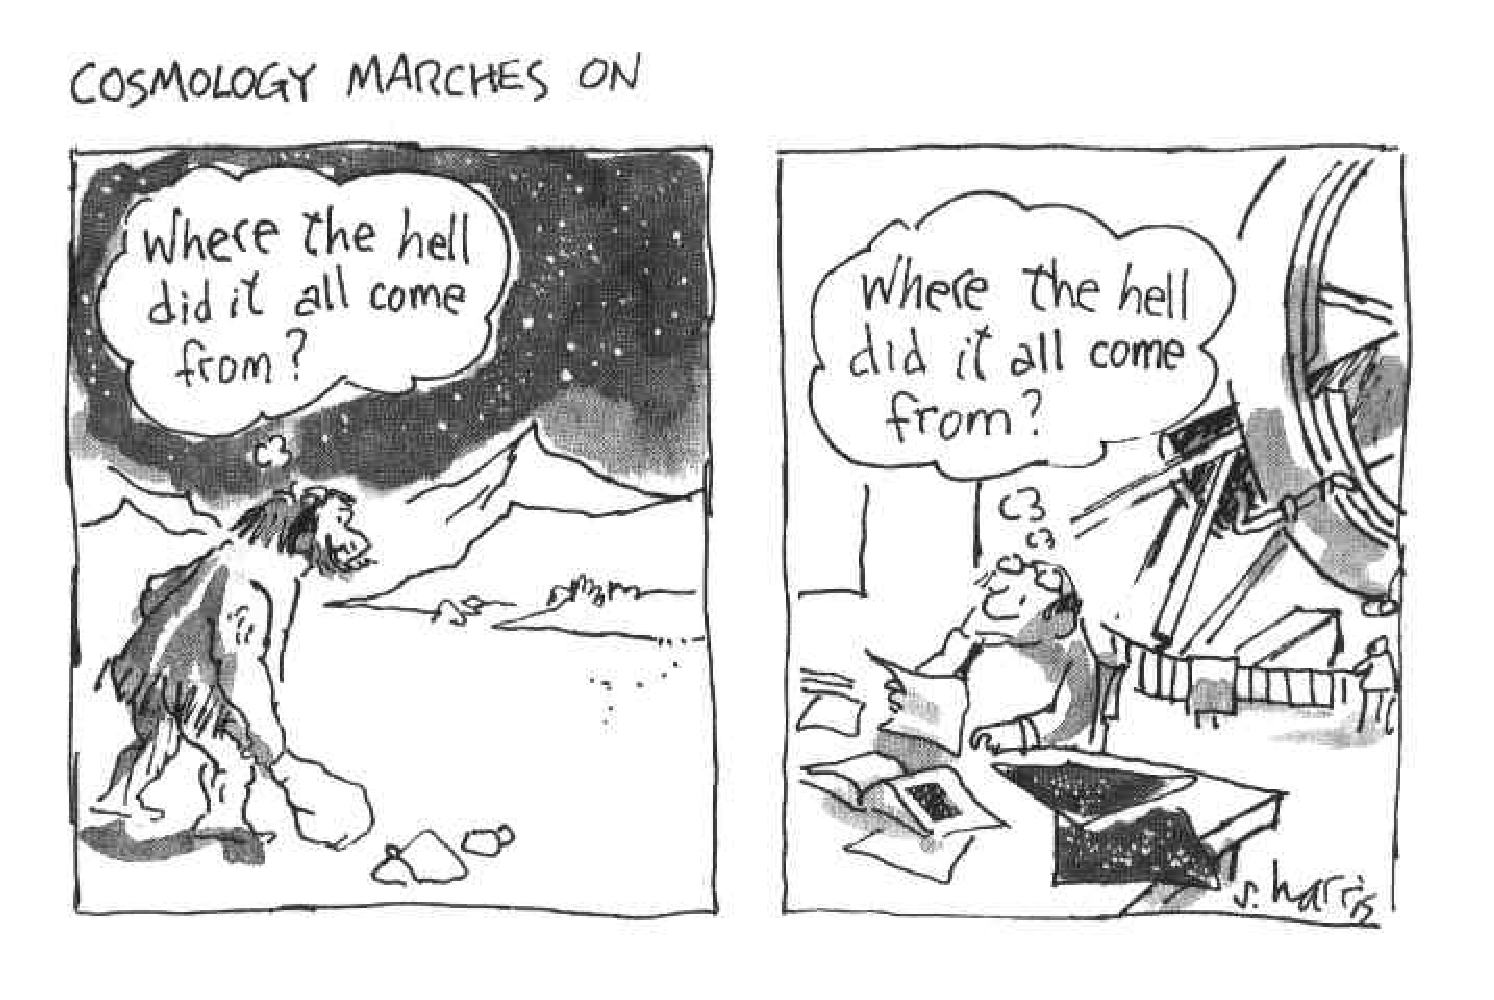
\includegraphics[height=8cm]{ambsthermopict/cosmology.eps} 
} 
\caption{Cosmology theories}
\label{cosmologytheory} 
\end{figure}



\begin{figure}[bhpt] 
\centerline{ 
\includegraphics[height=8cm]{ambsthermopict/cosmology2.eps} 
} 
\caption{Big Bang expansion}
\label{bigbang2} 
\end{figure}



\fi  % --- end moved Cosmology block ---

\part{World of ThermoDynamics}

\begin{quote}\itshape
The same RNS dynamics that explains Joule's experiment, refrigerators and
heat engines opens onto a much wider world: chemical reactors and combustion
engines (already touched on in the Reactive Flow chapter), living cells and
metabolic networks, climate systems and weather, the chemical engineering of
the process industry, traffic flow on highway networks, and the flow of money
and goods in an economy. Each of these is, at the level of its underlying
mathematics, a continuum flow with dissipation --- and each can be studied
with the same RNS apparatus, with the appropriate constitutive laws written
in. The four chapters that follow --- Information, Traffic Flow, Economy,
and (implicit, awaiting their own browser-runnable simulators) biology,
process industry, climate --- are intended as openings onto that world,
not as a closed catalogue.
\end{quote}

% --- bridge chapters moved here from Part I (Chemical Bonding, Blackbody Radiation) ---
\chapter{ThermoDynamics of Chemical Bonding}\label{ch:bonding}

\small
\begin{quote}
The bond is not a state. It is the trace, on the equilibrium surface, of a
process that took the system from one RealQM minimum to another and dissipated
the difference into the surrounding bath.
\end{quote}
\begin{quote}
\itshape The really fundamental thing is the interaction of electrons and
nuclei, which is governed by Coulomb's law. (Schr\"odinger, 1926)
\end{quote}
\normalsize

\section{The Bond as State vs the Bond as Event}

The classical thermodynamic description of a chemical bond consists of a few
state-function numbers --- a bond enthalpy $\Delta H_{\mathrm{bond}}$, a bond
entropy $\Delta S_{\mathrm{bond}}$, a free energy $\Delta G = \Delta H -
T\Delta S$ and the equilibrium constant $K = \exp(-\Delta G/RT)$ that decides
whether the bond exists at temperature $T$. The framework is silent on the
\emph{process} by which the bond forms. It encodes the released energy as a
state-function difference and the multiplicity loss as a state-function
difference, with the actual bonding event reduced to a discontinuous jump on
the equilibrium surface. There is no mechanism in it for how the energy is
released, or where it goes, or why an entropy decreases when two free atoms
become one bound molecule.

The view taken in this volume, and consistent with the with-Dynamics framing
of Chapter~\ref{ch:withwithout}, is different. The bond is not a state but
an \emph{event}: a process that takes the system from one RealQM minimum
(two separated atoms with their own electron territories) to another RealQM
minimum (a bonded molecule with overlapping electron territories between the
two nuclei), with the energy gap between the two minima dissipated into the
bath through the same molecular-scale Joule pattern that organises the rest
of this book. The state-function bookkeeping of classical thermodynamics
records the result; the dynamics records the process.

\section{The Atomic-Scale Energy Gap (RealQM Input)}

The energy gap between the two configurations is supplied by Volume~VI of
this programme, \emph{Real Quantum Mechanics} (RealQM)~\cite{RealQM2026}.
In the RealQM formulation, an $N$-electron system is described by a sum of
one-electron wave functions on non-overlapping spatial domains separated by
free (Bernoulli) boundaries, with ground states minimising the ordinary
Coulomb energy --- no configuration space, no antisymmetry postulate.

For the two-atom problem, two minima of the Coulomb energy functional
typically exist:

\begin{itemize}
\item A \emph{separated} minimum: the two atoms sit at large internuclear
distance $R \to \infty$ with their electron territories disjoint and
spherically symmetric about each nucleus. The total energy is
$E_{\mathrm{sep}} = E_A + E_B$, the sum of the isolated-atom energies.

\item A \emph{bonded} minimum: the two atoms sit at the equilibrium bond
distance $R_{\mathrm{eq}}$ with their electron territories rearranged so as
to overlap in the internuclear region, screening the proton--proton
repulsion and pulling both nuclei into the shared electron density. The
total energy is $E_{\mathrm{bond}}$, below $E_{\mathrm{sep}}$ by the
\emph{bond dissociation energy}
\begin{equation}
  D_e \;=\; E_{\mathrm{sep}} - E_{\mathrm{bond}} \;>\; 0.
  \label{eq:De}
\end{equation}
\end{itemize}

For $\mathrm{H}_2$ the RealQM calculation reproduced in Vol~VI gives $D_e
\approx 0.17\,\mathrm{Ha}$ at $R_{\mathrm{eq}} \approx 1.4\,\mathrm{au}$, in
agreement with the experimental value $4.75\,\mathrm{eV}$. The gap is a
deterministic property of the Coulomb energy functional --- it requires no
statistics, no probability interpretation, no microstate counting. Whatever
``bond energy'' the classical thermodynamic tables list for H--H, RealQM
computes from first principles.

\section{The Joule Pattern at Molecular Scale}

The bonding event, viewed as a dynamical process, follows the same
three-stage Joule pattern that organises Chapters \ref{ch:joule},
\ref{ch:refrig} and \ref{ch:piston}:

\begin{enumerate}
\item \textbf{Internal energy reservoir.} The two separated atoms together
hold an electronic configuration energy $E_{\mathrm{sep}}$. This is the
RealQM analogue of the high-pressure gas in Joule's left chamber: a stored
internal energy waiting to be released.

\item \textbf{Conversion to bulk kinetic energy.} As the atoms approach and
the electron territories rearrange, the energy gap $D_e$ is released by the
electronic system into the \emph{nuclear} degrees of freedom: first as
relative translational kinetic energy of the two approaching nuclei, then,
once they fall into the bonded minimum, as oscillatory kinetic energy of
the newly formed vibrational mode of the diatomic molecule. The energy is
not yet heat --- it is coherent kinetic motion of a single oscillator. This
is the analogue of the bulk jet through the channel in Joule's experiment:
internal energy converted into directed bulk flow.

\item \textbf{Dissipation into the bath.} The vibrational mode of the
newly formed molecule does not stay coherent. It couples to surrounding
molecules through collisions, transferring quanta of vibrational energy
into translational kinetic energy of the bath in a sequence of irreversible
inelastic collisions. After a few mean-free-path times, the coherent
vibration has been thermalised: the originally localised energy $D_e$ has
become a tiny incremental heating of the surrounding gas. This is the
analogue of the turbulent dissipation in the receiving chamber of Joule's
experiment: directed bulk kinetic energy degraded into incoherent thermal
motion.
\end{enumerate}

The result is the same as the result reported by classical thermodynamics
--- a heat release of magnitude $D_e$ per bond formed --- but the mechanism
is now explicit. The energy was not magically transferred from one column
of a table to another; it was released by the electronic system, channelled
into a single coherent mode of nuclear motion, and then dissipated into the
bath by collisional coupling. The Joule pattern --- internal energy
$\to$ bulk kinetic energy $\to$ irreversible dissipation $\to$ heat ---
applies at molecular scale exactly as it applies at macroscopic scale.

\section{Macroscopic Heat Balance and the Reactive RNS Apparatus}

For a gas in which the bonding event is happening many times per unit
volume per unit time, the bookkeeping is the business of the reactive RNS
apparatus developed in Chapter~\ref{ch:reactive} (Chemistry: RNS with
Chemical Reactions). Each elementary reaction $\mathrm{A} + \mathrm{B} \to
\mathrm{AB}$ contributes:

\begin{itemize}
\item A source term in the species equation for $\mathrm{AB}$ and matching
sink terms for $\mathrm{A}$ and $\mathrm{B}$, with rate set by collision
frequency and the Arrhenius factor for any activation barrier.

\item A heat source in the internal-energy equation equal to $D_e$ per
reaction event, contributing to the local temperature rise.

\item A momentum redistribution (typically small for a near-equilibrium
reaction) reflecting the change in mean molecular weight of the gas.
\end{itemize}

The viscous dissipation $D = \int\!\int\mu_{\mathrm{mom}}|\nabla u|^2\,dx\,dt$
of the bulk flow is now joined by a \emph{reactive dissipation} from the
local relaxation of species gradients --- the chemical analogue of viscous
shear. Together they form the irreversibility of a reacting gas: the 2nd
Law in this setting is the statement that both contributions are positive
and that their sum equals the rate at which the chemical free energy stored
in unreacted species is degraded to heat.

\section{The Mysteries of Bonding Entropy Dissolved}

Several classical puzzles about bonding now have natural resolutions:

\begin{itemize}
\item \emph{Why is $\Delta S_{\mathrm{bond}}$ negative?} In the classical
framework this is mysterious: the bonded molecule has fewer ``microstates''
than two free atoms, so $\Delta S$ must be negative, but the framework
gives no reason \emph{why} the bonded molecule is the natural endpoint
despite the entropic penalty. In the with-Dynamics framework the question
dissolves: bond formation is the dissipative dynamics relaxing toward the
deeper RealQM minimum, with the released energy $D_e$ dissipated into the
bath. There is no microstate counting. The bond exists because the
$D_e$-deep minimum exists, and the dissipative dynamics finds it.

\item \emph{Why is the equilibrium constant $K = \exp(-\Delta G/RT)$?} In
the with-Dynamics framework this is the steady-state condition for the
reactive RNS: at temperature $T$, the forward reaction rate (driven by
$D_e$) and the backward rate (driven by thermal kinetic energy of bonded
pairs sufficient to climb out of the bonded minimum) balance when the
ratio of populations is set by the Boltzmann factor evaluated at the
bonded-minimum depth. No postulate is needed; the steady state of the
reactive flow gives the same answer that the classical state-function
bookkeeping was forced to postulate.

\item \emph{Where does the bond energy ``go''?} Into the bath, by the
three-stage Joule pattern: into vibrational kinetic energy of the newly
formed molecule, and from there by inelastic collisions into translational
kinetic energy of surrounding molecules. The same dissipation $D > 0$
that organises the rest of this book carries the bonding event from RealQM
to the macroscopic temperature.
\end{itemize}

The chemical bond, the most basic non-trivial chemical event, is therefore
the cleanest single illustration of why ThermoDynamics needs Dynamics. The
classical state-function description captures the bookkeeping; the
with-Dynamics description captures the bookkeeping \emph{and} the
mechanism, with RealQM supplying the energy gap and the Joule pattern at
molecular scale supplying the channel through which the gap is dissipated.

\chapter{ThermoDynamics of Blackbody Radiation}\label{ch:blackbody}

\small
\begin{quote}\itshape
A perfectly stable cavity, at rest at temperature $T$ in empty space,
fills with electromagnetic radiation of a spectrum that depends only on
$T$. The mystery is not the spectrum --- Planck wrote it down in 1900.
The mystery is the cutoff: why the high-frequency tail does not
diverge.
\end{quote}
\begin{quote}\itshape
The whole of the energy of the radiation is degraded into heat at a
rate that is finite, never infinite. (Planck, paraphrased)
\end{quote}
\normalsize

\section{The Mystery of the Cutoff}

The classical electromagnetic theory of a cavity in equilibrium with
its walls assigns equal energy $k_{\mathrm{B}}T$ to every standing-wave
mode. The number of modes between frequencies $\omega$ and $\omega +
d\omega$ grows as $\omega^2 d\omega$, so the predicted spectral energy
density grows as $\omega^2 k_{\mathrm{B}}T$ and the total energy
$\int_0^\infty \omega^2 k_{\mathrm{B}}T\,d\omega$ diverges --- the
\emph{ultraviolet catastrophe}. Real cavities of course hold finite
energy. The puzzle, in 1900, was where the high-frequency end of the
spectrum gets cut off.

Planck's resolution introduced an inseparable quantum of energy
$\hbar\omega$ per mode, with the Boltzmann factor
$\exp(-\hbar\omega/k_{\mathrm{B}}T)$ suppressing modes for which
$\hbar\omega \gg k_{\mathrm{B}}T$. The spectrum becomes
\[
  u(\omega,T) \;=\; \frac{\hbar\omega^3/\pi^2 c^3}{\exp(\hbar\omega/k_{\mathrm{B}}T) - 1},
\]
finite for every $T$, with a sharp drop at $\omega \sim
k_{\mathrm{B}}T/\hbar$ that places the cutoff in the right physical
place. The mathematics works. The physical picture --- \emph{what
happens to the high-frequency radiation that would have been there
without the cutoff} --- was less clear at the time and is still treated
in many textbooks as merely a statistical consequence of mode
counting.

\section{The Cutoff as Dissipation}

Read in the with-Dynamics framing of this volume, the Planck cutoff is
the radiative analogue of the viscous cutoff in turbulent flow.

In turbulent compressible flow at high Reynolds number, the
deterministic continuum equations would describe a flow with structure
on all scales down to zero. The flow that is actually realised, in
finite resolution, has a cutoff at the viscous scale --- the scale
below which the molecular viscosity becomes comparable to the inertial
forces and the energy that would have cascaded to still smaller scales
is instead converted to internal energy. The dissipation
$D = \int\!\int \mu_{\mathrm{mom}}|\nabla u|^2\,dx\,dt$ of this volume
is the cumulative rate of that conversion. Without the cutoff the
cascade would run to infinity; with the cutoff it terminates by
turning small-scale kinetic energy into heat.

The same pattern governs the radiation field in a cavity. The
classical (unquantised) Maxwell theory predicts modes at arbitrarily
high frequency, each carrying its equipartition $k_{\mathrm{B}}T$. The
field that is actually realised has a cutoff at the quantum scale ---
the scale at which a single quantum $\hbar\omega$ exceeds the thermal
energy $k_{\mathrm{B}}T$ and the corresponding modes can no longer be
populated. The high-frequency radiation that would have been there
without the cutoff is absorbed by the walls and converted to heat ---
exactly the radiative counterpart of the small-scale turbulent kinetic
energy being absorbed at the viscous scale and converted to heat.

\begin{center}
\begin{tabular}{l|l}
\textbf{Turbulence (RNS)} & \textbf{Blackbody radiation} \\
\hline
inertial flow at small scales & high-frequency modes \\
viscous cutoff at $\ell \sim (\nu^3/\epsilon)^{1/4}$ &
quantum cutoff at $\omega \sim k_{\mathrm{B}}T/\hbar$ \\
small-scale kinetic energy $\to$ heat &
above-cutoff radiation $\to$ heat \\
dissipation $D = \int\mu|\nabla u|^2\,dx\,dt \geq 0$ &
absorption rate $\geq 0$ \\
2nd Law as inevitability of $D > 0$ &
2nd Law as inevitability of absorption \\
\end{tabular}
\end{center}

The cutoff is what makes both phenomena \emph{finite}. Without it, the
cascade would run unbounded and the field would carry infinite energy.
The mechanism is the same in spirit: a structural barrier below which
the small-scale degrees of freedom can no longer be supported, and
above which the energy that would have populated them is delivered
instead to the thermal bath.

\section{Computational Blackbody}

The same computational framing that organises this volume applies. A
finite-precision solver of the Maxwell equations on a cavity at
temperature $T$ has a natural cutoff set by its spatial resolution: it
cannot represent modes with wavelength shorter than its mesh spacing,
and the radiation energy that would have lived in those modes is
re-deposited, by the discretisation, as a heating source in the bath.
The Planck cutoff is, in this reading, not a quantum-mechanical
postulate but the cutoff that any finite-resolution representation of
the field must impose --- realised in Nature by whatever physical
process limits the resolution at very short wavelength, and realised
on a computer by the mesh.

This view is developed in detail in the author's earlier
\emph{Computational Black-Body Radiation}~\cite{blackbody}. The
present chapter records that the Planck cutoff and the viscous cutoff
of turbulent RNS are two instances of the same with-Dynamics
mechanism: small-scale degrees of freedom that the underlying
continuum equations \emph{would} support, and that finite resolution
\emph{does not}, deliver their energy as heat. The 2nd Law, in this
joint reading, is the inevitability of that delivery --- in
turbulence, in radiation, and in every other context in which a
continuum field is realised at finite resolution.


% --- chapters moved here from Part I (Refrig+HP, Piston) and Part II (Transformations) ---
\chapter{Transformations of Energy}



\small

\begin{quote}
%Dieu a choisi celuy qui est... le plus simple en hypotheses et le plus riche 
%en phenomenes 
God has chosen that which is the most simple in 
hypotheses and the most rich in phenomena. (Leibniz, 
Discours de m\'etaphysique, VI, 1686)
\end{quote} 

%\begin{quote} The ordinary man (or woman) thinks he knows what time is
%but cannot say. The learned man, physicist or philosopher, is not sure
%he knows but is ready to write volumes on the subject of his
%speculation and ignorance. (David Landes in \emph{Revolution in Time} 1983)
%\end{quote}

\begin{quote}
The sight of day and night, and the months and the revolutions of the
years, have created number and have given us conception of time,
and the power of inquiring about the nature of the Universe. (Plato 
in \emph{Timaeus})
\end{quote}

\begin{quote}
... in a purely mechanical world, the tree could become a shoot 
and a seed again, the butterfly turn back into a caterpillar, and the
old man into a child. No explanation is given by the mechanistic doctrine
for the fact that it does not happen. (Ostwald)
\end{quote}

\begin{quote} ... a complete explanation of the arrow requires
explaining why the universe started out as it did. It is a problem
in cosmology. (Hawking)
\end{quote}
\normalsize

\section{Kinetic Energy and Heat Energy}

\emph{Thermodynamics} is fundamental in a wide range of phenomena from
macroscopic to microscopic scales. 
Thermodynamics essentially concerns the interplay between
\emph{kinetic energy} and  \emph{heat energy} in a \emph{gas} or \emph{fluid},
where heat energy is a form of small scale kinetic energy.
Thermodynamics thus concerns transformations between large scale
kinetic energy and small scale kinetic energy in the form of heat.
Large scale kinetic energy, or \emph{mechanical energy}, 
may generate heat energy by 
\emph{compression} or \emph{turbulent dissipation}. 
Heat energy may generate (large scale) kinetic energy by \emph{expansion}, but
not through a \emph{reverse} process of turbulent dissipation. 
Thermodynamics is closely connected to the dynamics of \emph{slightly viscous}
and \emph{compressible} gases, since substantial compression and 
expansion can occur in a gas, but less in fluids (and solids).

  
\section{Cosmology and Big Bang}

\emph{Cosmology} is the scientific study of the large scale properties of the 
\emph{Universe} as a whole, including its   
origin, evolution and ultimate fate. 
%The prevailing theory is 
%the so-called idea of a Big Bang where intense heat generated a lot
%of kinetic energy collected in galaxies of stars
%moving away from each other with velocity. 
The \emph{Big Bang} model postulates that 12 to 14 billion years ago,
the universe was in a very hot very dense 
state, which expanded along with galaxies and stars being 
formed by gravitation from variations in density, see Fig. \ref{bigbang}.
 It is believed that
we can see remnants of the hot 
dense matter as the now very cold cosmic microwave background radiation, 
which still pervades the universe as a slightly varying glow across 
the entire sky, see Fig. \ref{cobe}, a discovery made 
by the Cosmic Background Explorer COBE-telescope, which gave
the Nobel Prize in 2006 to John Mather and George Smoot.
Cosmology is basically a very (very) large scale application of thermodynamics
as an interplay of mass, momentum and energy governed by 
gravitational and inertial forces and driven by nuclear reactions.
% \begin{figure}[bhpt]
% \centerline{
% \includegraphics[height=8.0cm]{theoryoftimepict/bigbang.eps}
% }
% \caption{Thermodynamics of Big Bang from $10^{-41}$ seconds to 15 billion years.}
% \label{bigbang}
% \end{figure}   % --- removed: theoryoftimepict/bigbang.eps not in repo ---
\begin{figure}[bhpt] 
\centerline{ 
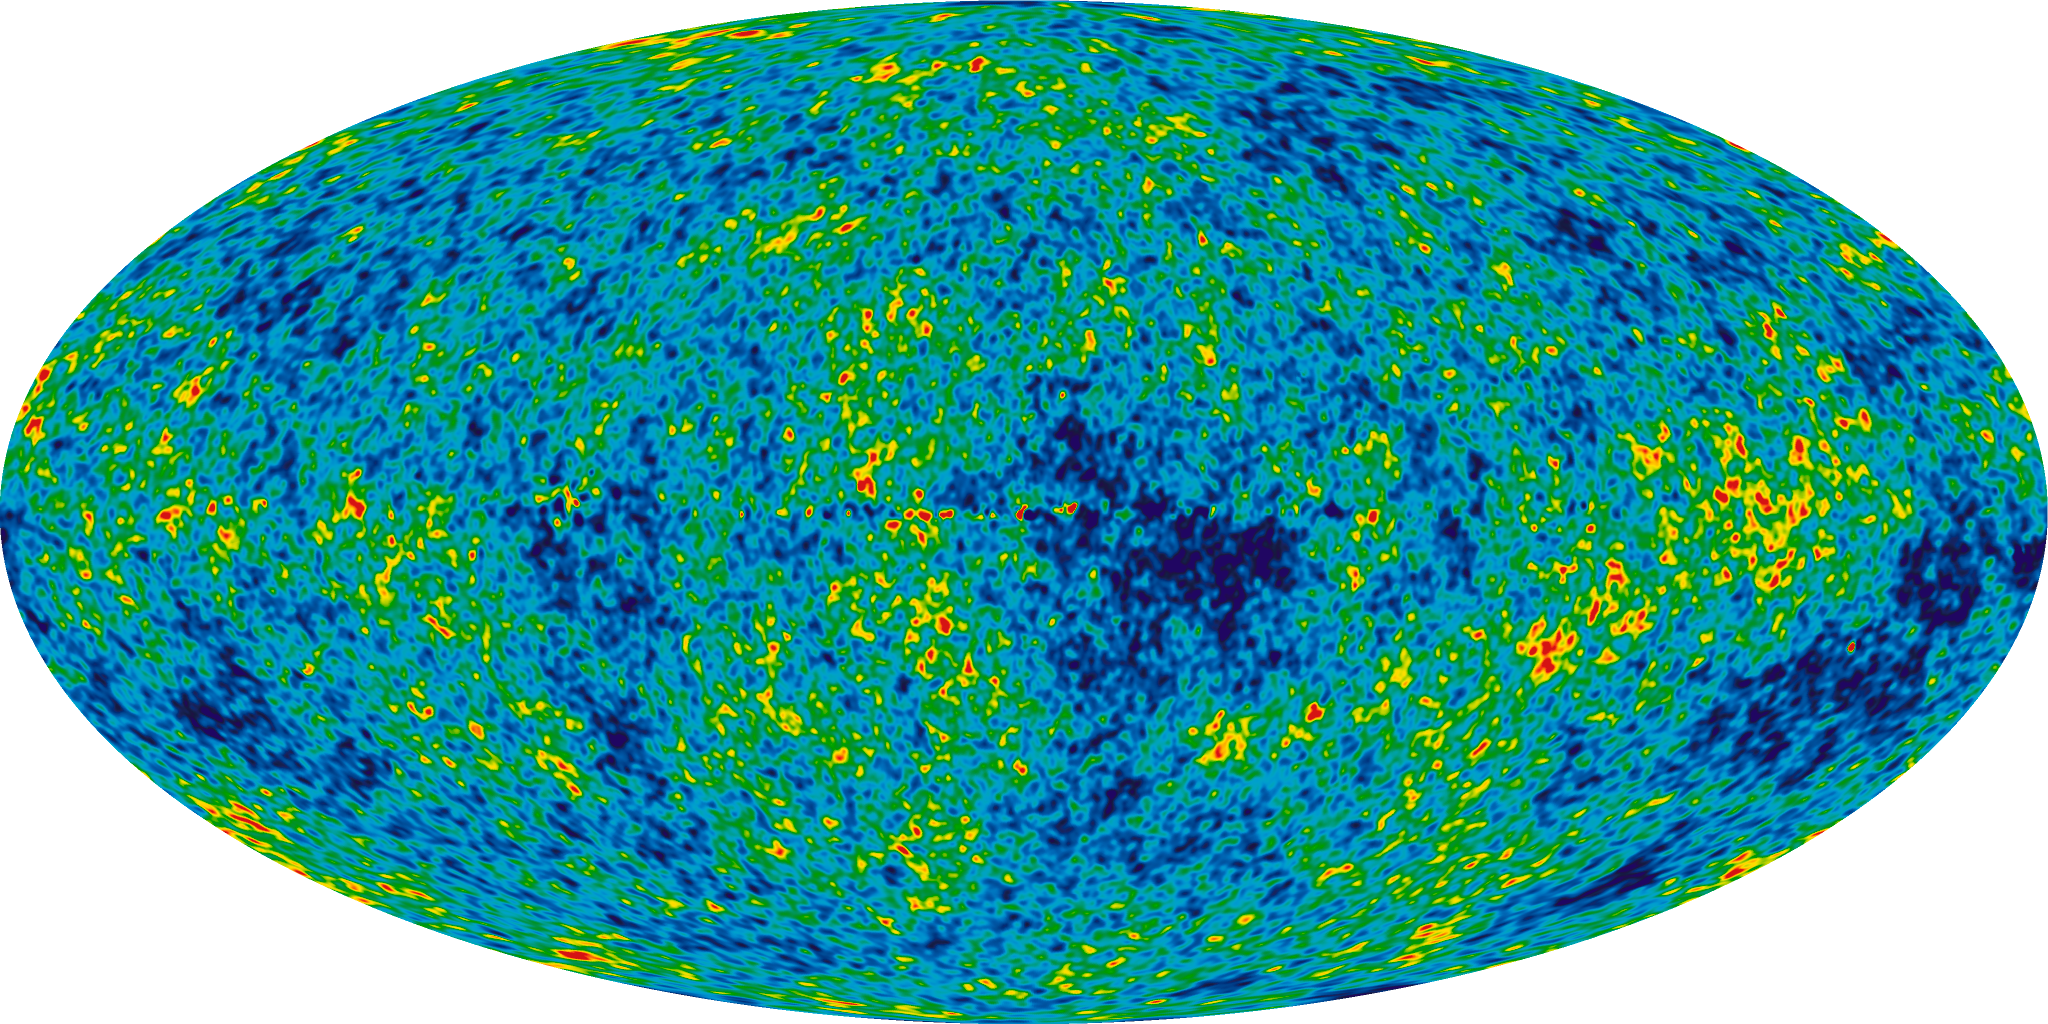
\includegraphics[height=4.0cm]{ambsthermopict/CMB_ILC_Map300.eps} 
} 
\caption{Cosmic back-ground radiation
according to COBE.}
\label{cobe} 
\end{figure}



%The Big Bang Model rests on the two theoretical pillars of
%Einstein's General Relativity and the Cosmological Principle.
%The key concept of General Relativity is that matter tells space how 
%to curve, and space tells matter how to move. 
%The Cosmological Principle states that matter in the universe is 
%homogeneous and isotropic when averaged over very large scales,
%supported by the observation that the cosmic microwave background 
%radiation has a temperature which 
%is highly uniform over the entire sky. 
%This fact strongly supports the notion that the gas which emitted this radiation 
%long ago was very uniformly distributed.

\section{Astronomy and Nuclear Energy}

The \emph{stars} were formed in the early Universe 
by accretion of mass by gravitational collaps 
increasing the temperature of a central core and thus igniting 
the star in a nuclear fusion process
with first deuterium and then hydrogen being transformed to helium under
intense release of energy (according to Einsteins famous
formula $E=mc^2$) increasing the pressure and counterbalancing
the gravitational collaps. \emph{Planets} may be formed 
from heavier atoms and molecules created in nuclear processes in stars,
and under favorable conditions give rise to (intelligent) \emph{life}
and theories of thermodynamics. 
Stars of 0.4-10 times the mass of our own Sun
expand into red giant very bright stars, when 
the supply of hydrogen in the core is empty and fusion starts in an 
outer core. Our own Sun thus eventually will swallow the Earth
into a fusion process, but this is estimated to be a couple of billion
years away. The thermodynamics of the Sun thus is the basis
of both life and death of the Earth.

% \begin{figure}[bhpt]
% \centerline{
% \includegraphics[height=8.0cm]{theoryoftimepict/impact.eps}
% }  % --- removed: theoryoftimepict/impact.eps not in repo; caption follows but unused ---
\iffalse
\begin{figure}[bhpt]
\centerline{
\includegraphics[height=8.0cm]{theoryoftimepict/impact.eps}
}
\caption{Asteroid impact on the surface of the Earth with irreversible transfer of large
scale kinetic energy
into small scale kinetic energy in the form of heat energy.}
\label{impact}
\end{figure}
\fi  % --- end removed impact.eps figure block ---



\section{Geology and Global Warming}
	
\emph{Geology} or earth science contains the subfields of
geophysics, glaciology, 
%petrology, seismology, 
volcanology, climatology and meteorology 
connecting to the the central issue of 
the thermodynamics of \emph{global warming}. Computational 
simulation of global climate change has a very important role to play
to find out what actions are beneficial for 
sustainable development and long-time survival. 



\begin{figure}[bhpt] 
\centerline{ 
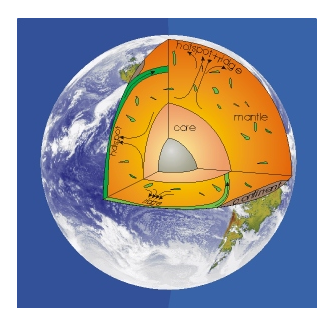
\includegraphics[height=8.0cm]{ambsthermopict/earth.eps} 
} 
\caption{The Earth}
\label{nse_people} 
\end{figure}

\begin{figure}[bhpt] 
\centerline{ 
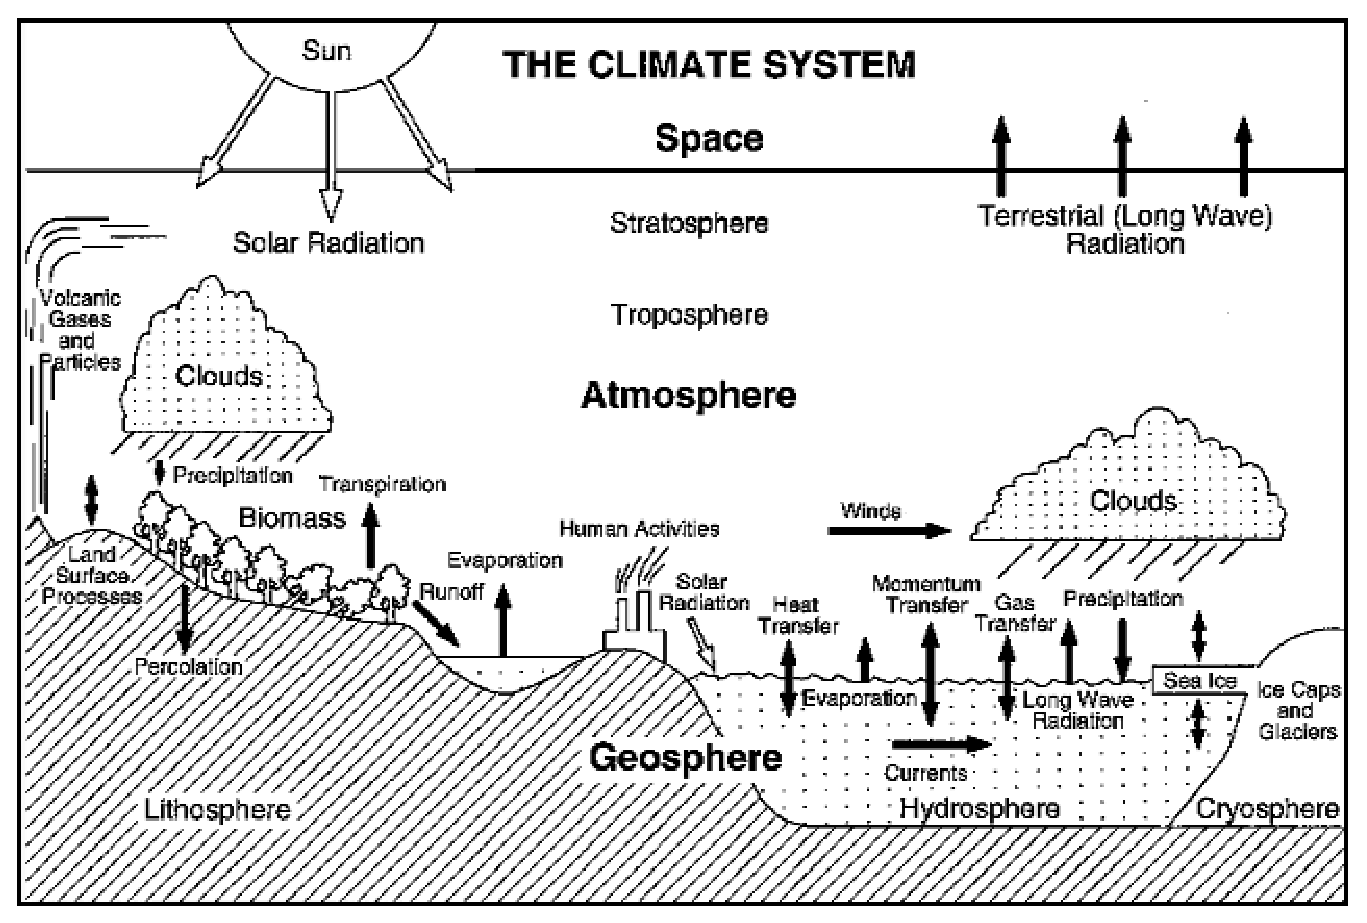
\includegraphics[height=6.0cm]{ambsthermopict/climate.eps} 
} 
\caption{Global heat balance.}
\label{nse_people} 
\end{figure}


\section{Black Body Radiation and the Sun}


A \emph{black body} absorbs incoming white light of all frequencies, 
from high frequency ultraviolet to low frequency infrared, but only radiates
low frequency light (with color depending on 
the temperature of the body).  This is the basis of the gross energy balance
of the Earth absorbing white light from the hot Sun and radiating 
low frequency light into empty space. One can view  
black body absorption/emission as an (irreversible) 
thermodynamic process transforming high frequency light energy  
to low frequency (long wave) light energy \cite{blackbody}. 


\begin{figure}[bhpt] 
\centerline{ 
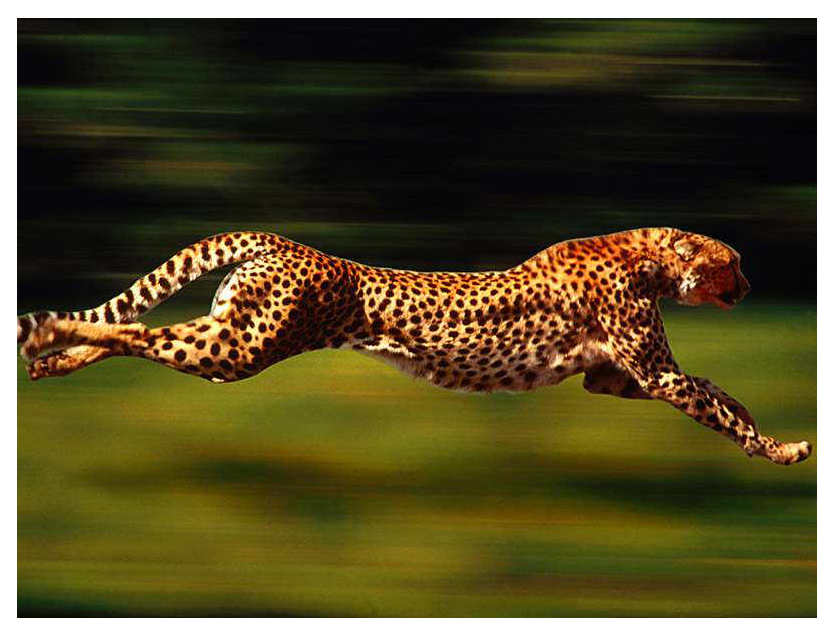
\includegraphics[height=6.0cm]{ambsthermopict/gepard.eps} 
} 
\caption{Life in action.}
\label{nse_people} 
\end{figure}


\begin{figure}[bhpt] 
\centerline{ 
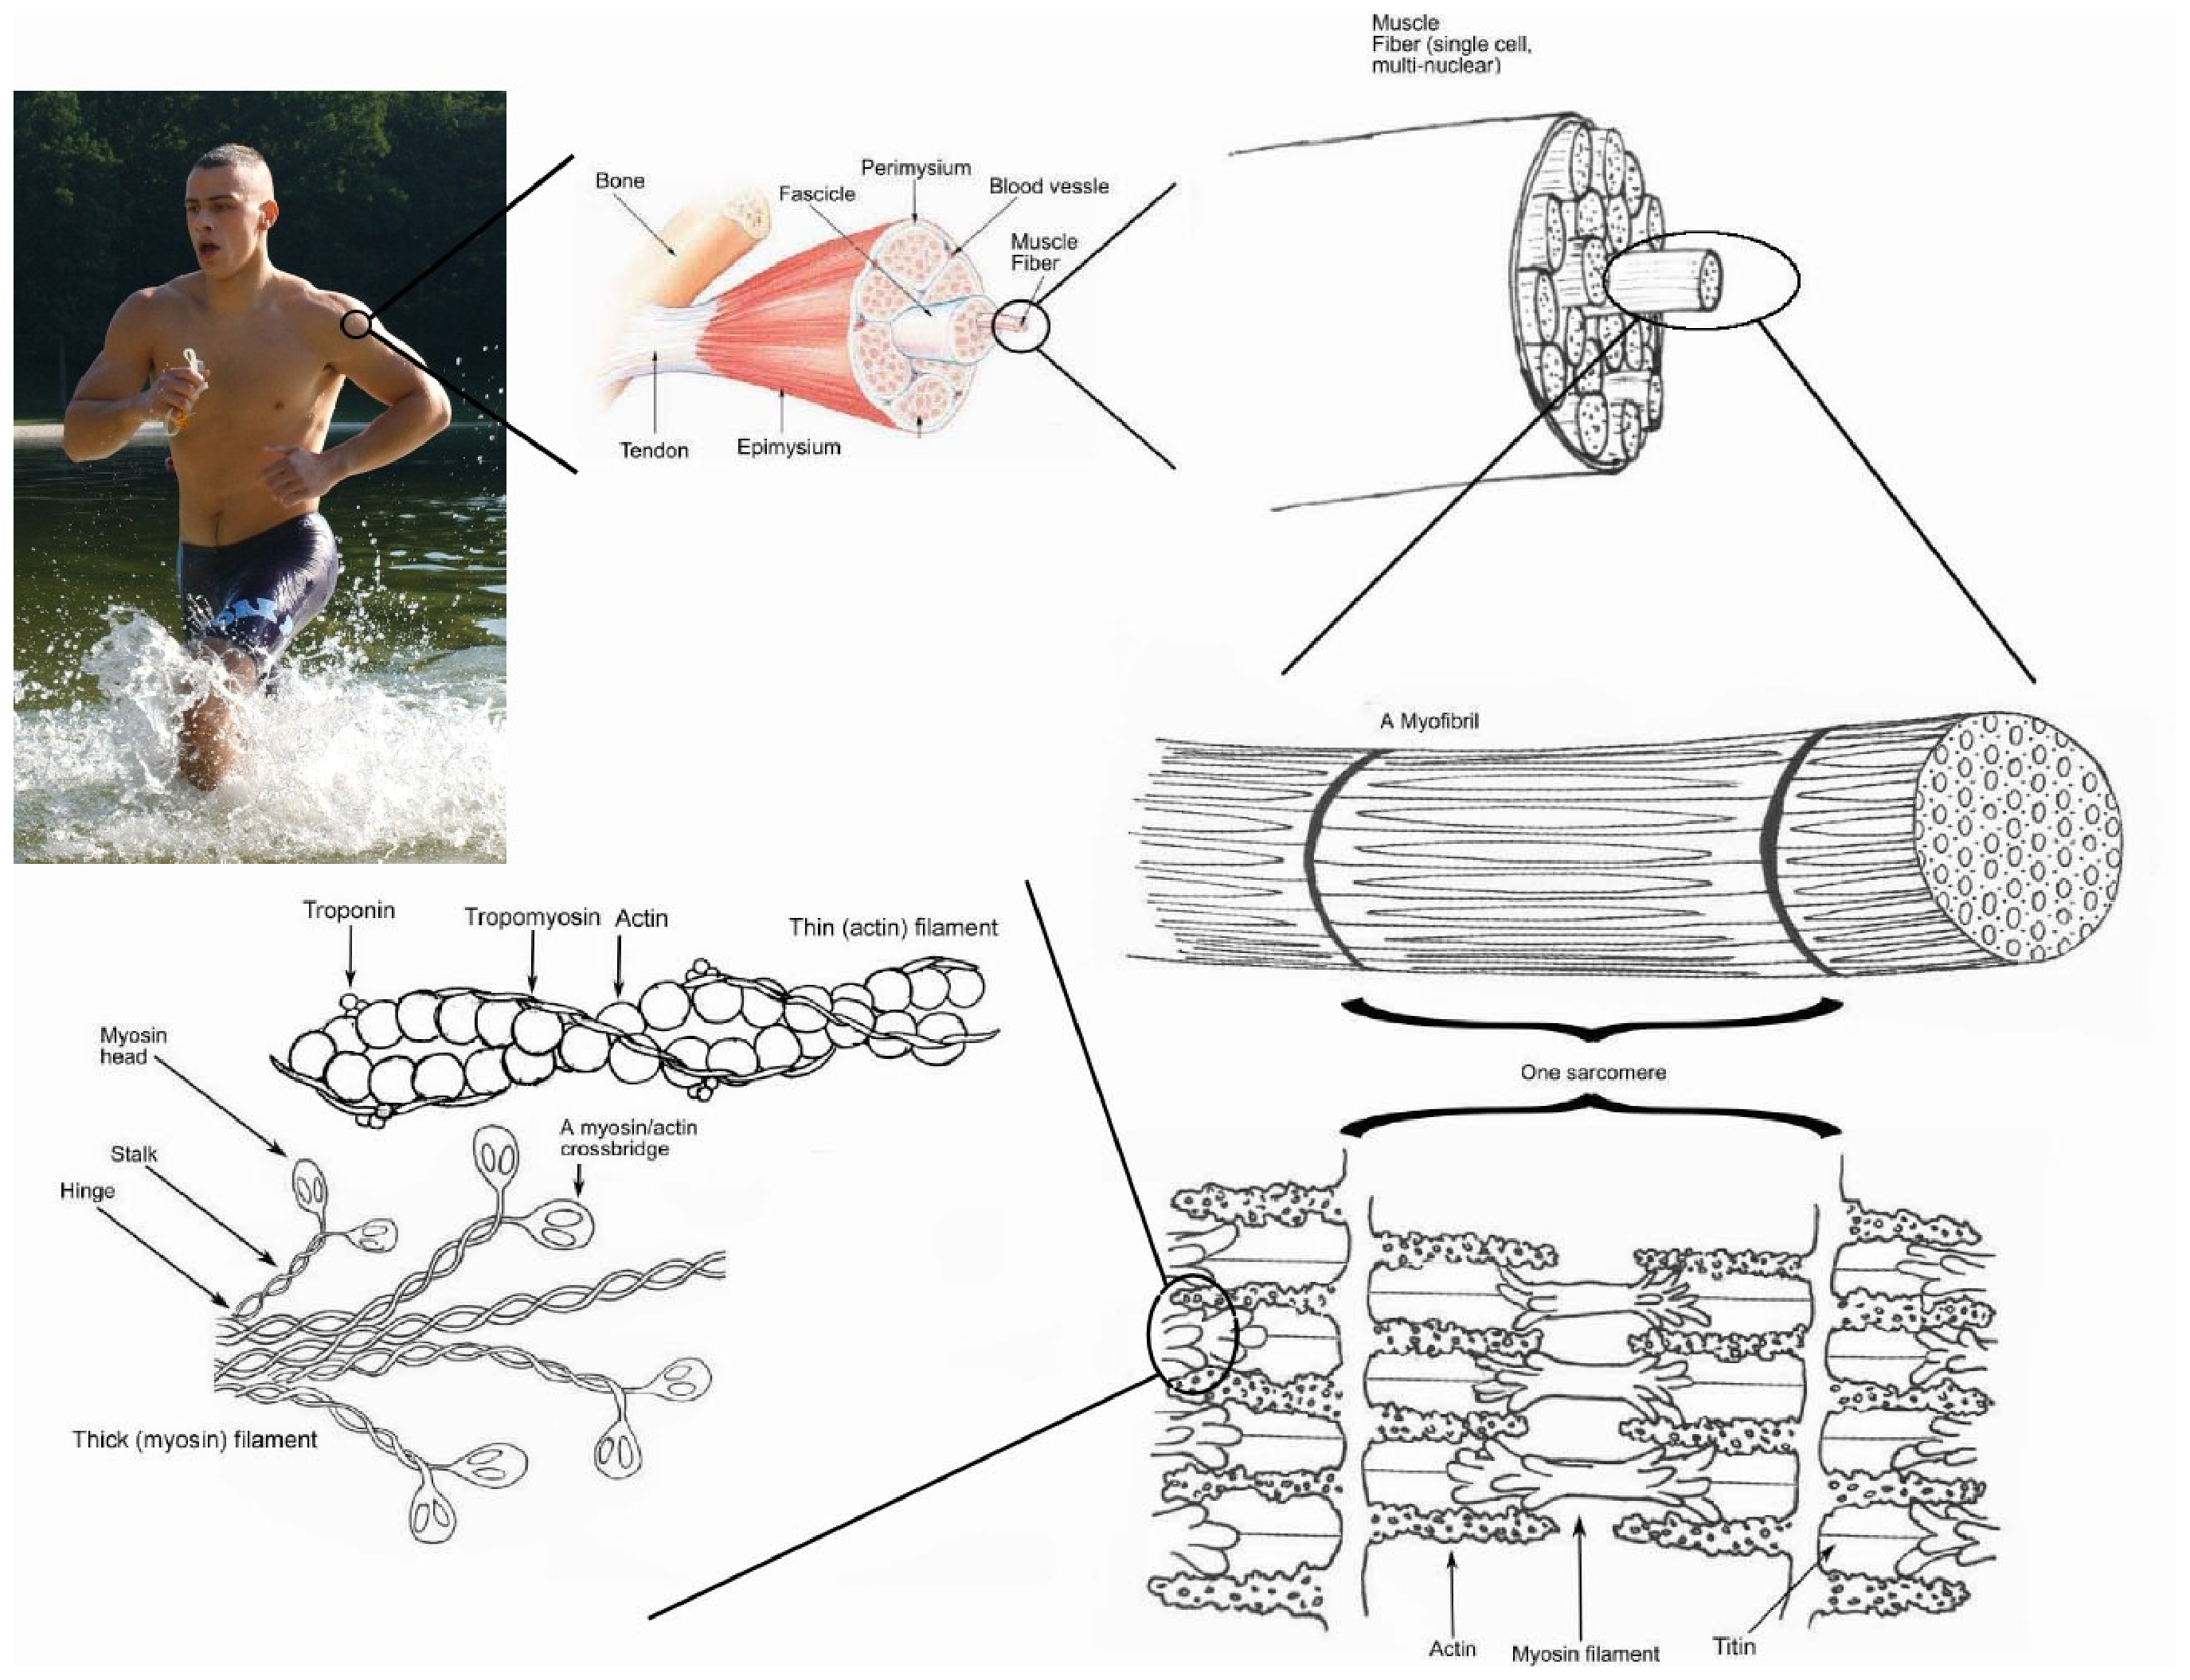
\includegraphics[height=8.5cm]{ambsthermopict/muscle.eps} 
} 
\caption{Muscle contraction by actin-myosin twitch fueled by ATP.}
\label{nse_people} 
\end{figure}




\section{Biology and Life}

Most forms of biological processes build on conversion of
chemical energy into heat and kinetic energy,
and thus ultimately on Solar energy converted to chemical energy 
in the \emph{photo-synthesis}.


\emph{Muscle contraction}  
occurs when a muscle fiber generates tension through
\emph{actin and myosin cross-bridge cycling} shortening the fiber
fueled by \emph{Adanenosine TriPhosphate ATP}.
Locomotion in most higher animals is possible only 
through the repeated contraction of many muscles at the correct times 
controlled by the central nervous system,
the brain and spinal cord. Voluntary muscle contractions 
are initiated in the brain, while the spinal cord initiates involuntary 
reflexes.

The emergence of biological life may naively appear to contradict the 2nd 
Law in its classical form, by creating ordered structures out of disordered, 
while the death of a living organism when order dissolves into disorder,
reflects the classical 2nd Law very well. We shall see that in the
new formulation of the 2nd Law not relying on notions of 
ordered/unordered, there
is nothing (in principle) that prevents ordered structures to develop 
from unordered
(for example in Irak), assuming there is some input of energy (oil). 
%which is kind of a happy message to everybody who is not an extreme pessimist.
%This is one of many indications that
%the classical from of the 2nd Law poses
%difficulties.

\begin{figure}[bhpt] 
\centerline{ 
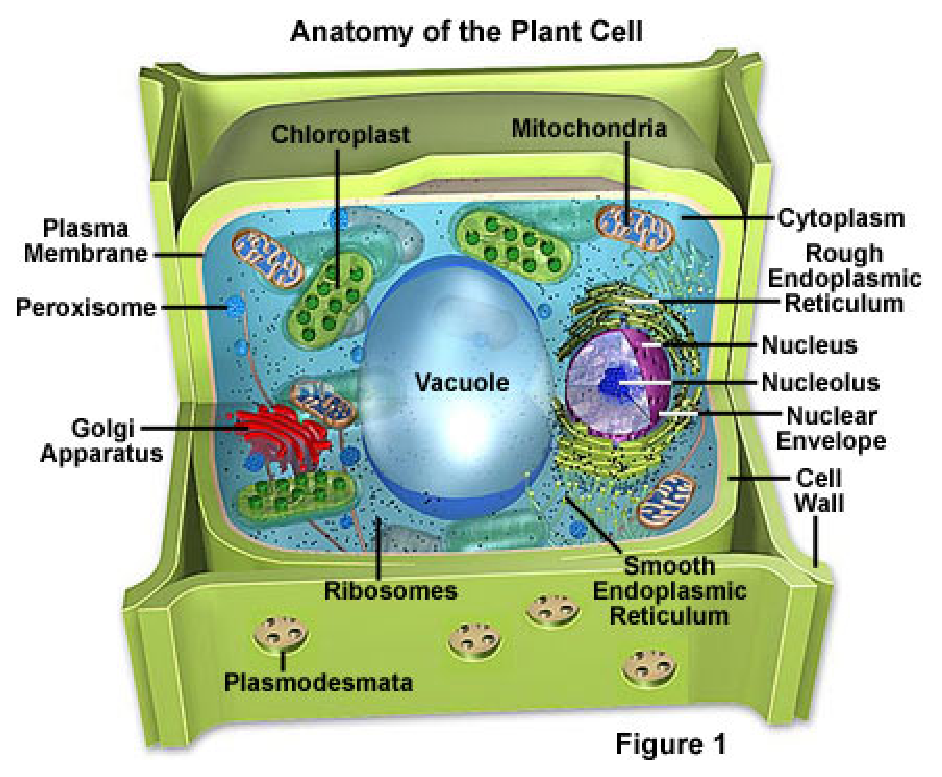
\includegraphics[height=6.0cm]{ambsthermopict/plantcell.eps} 
} 
\caption{Inside a plant cell.}
\label{nse_people} 
\end{figure}


\section{Molecular Biology and Protein Folding}

Biology builds on cell microbiology based on the thermodynamics of
chemical reactions of \emph{protein
synthesis} from amino acid molecules according to
the instructions of \emph{DNA}. Computational thermodynamics of the cell
is becoming an increasingly important tool in medicine and drug design.

%\begin{figure}[bhpt] 
%\centerline{ 
%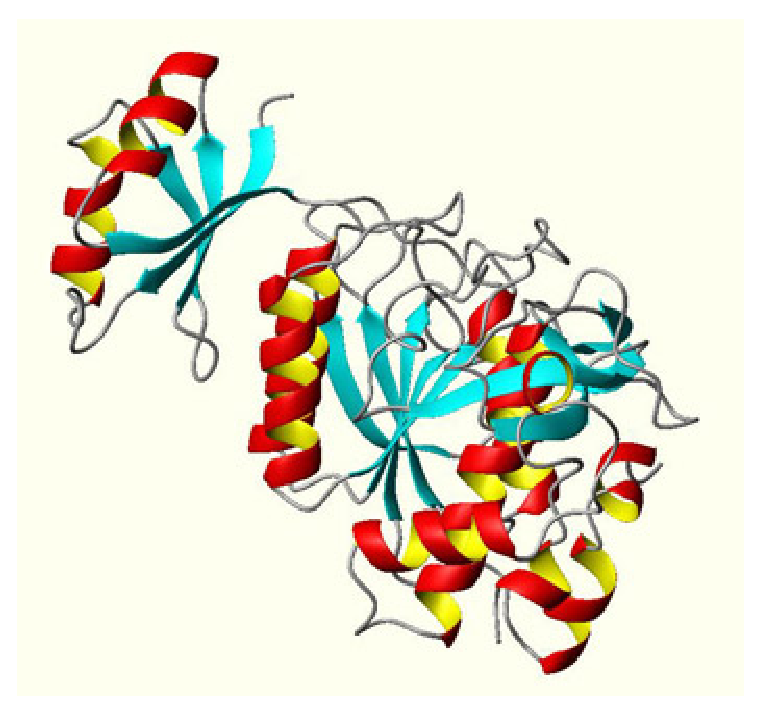
\includegraphics[height=8.0cm]{ambsthermopict/proteinfolding.eps} 
%} 
%\caption{Protein folding}
%\label{nse_people} 
%\end{figure}

%\begin{figure}[bhpt] 
%\centerline{ 
%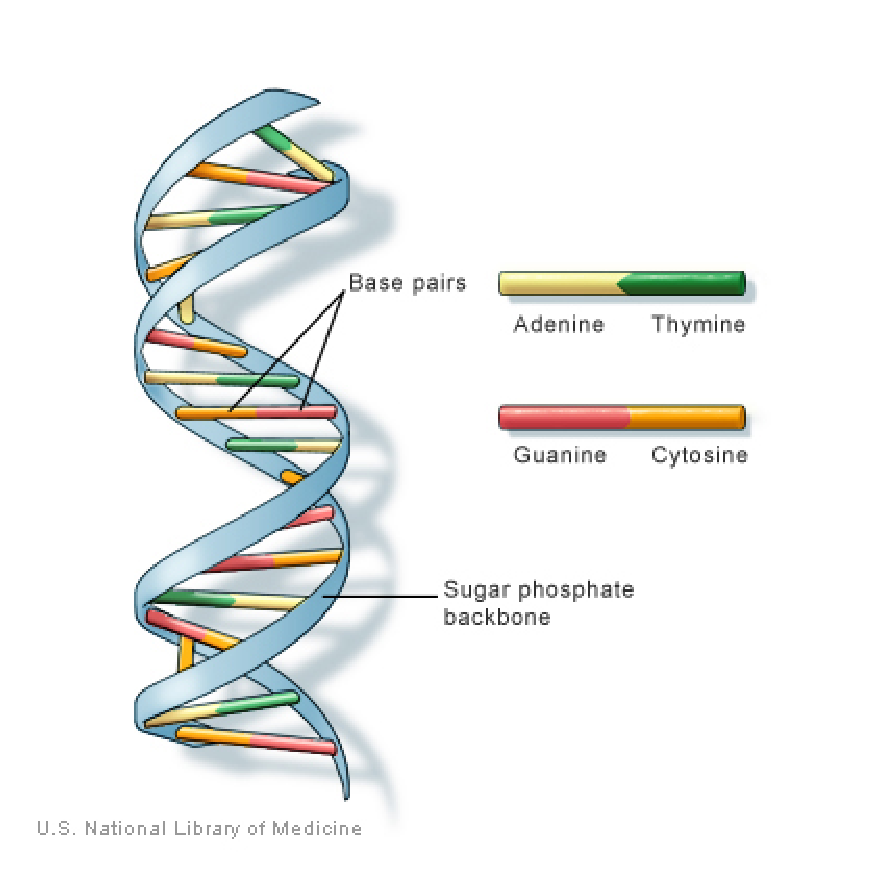
\includegraphics[height=8.0cm]{ambsthermopict/doublehelix.eps} 
%} 
%\caption{The double helix of DNA}
%\label{nse_people} 
%\end{figure}



 
\section{Quantum Physics and Chemistry}

The thermodynamics of chemical reactions and radiation
build on the \emph{quantum mechanics}
of electrons, and the thermodynamics of nuclear reactions build
on quantum electrodynamics of elementary particles. Computational solution
of the equations of quantum mechanics presents a tough challenge, 
because of the richness of the the wave function solution 
with in principle three independent 
space coordinates for each particle (electron) involved. 
Methods
reducing the dimensionality are today routinely used in massive
computations in \emph{quantum chemistry}, and could open to new insights
of the nature of the quarks of elementary particle physics.
%\cite{compquantum}. 

 




\section{Energy Generation and Consumption}

Our \emph{industrial society} is based on production and
consumption of energy in thermodynamic energy conversion processes of 
the form:

\begin{itemize}

\item nuclear/fossile/biological/chemical $\rightarrow$ heat/kinetic/electric, 

\item wind/wave kinetic $\rightarrow$ electric,

\item solar radiation $\rightarrow$ heat/electric.
\item electric $\rightarrow$ heat/kinetic.  
\end{itemize}
In all conversion of energy, minimization of \emph{losses} into useless heat is 
of prime concern, for which computational thermodynamics opens new
possibilities.
\section{Heat Engines and Industrialization}

%The early development of thermodynamics was motivated by the need of 
%understanding the steam engine, underlying the industrialization
%of the Western World in the 19th century.

The industrial society
of the 19th century was built on the use of \emph{steam engines}, and the 
initial motivation to understand thermodynamics came from a need to
increase the efficiency of steam engines for conversion of heat energy to
useful mechanical energy. 
\begin{figure}[bhpt] 
\centerline{ 
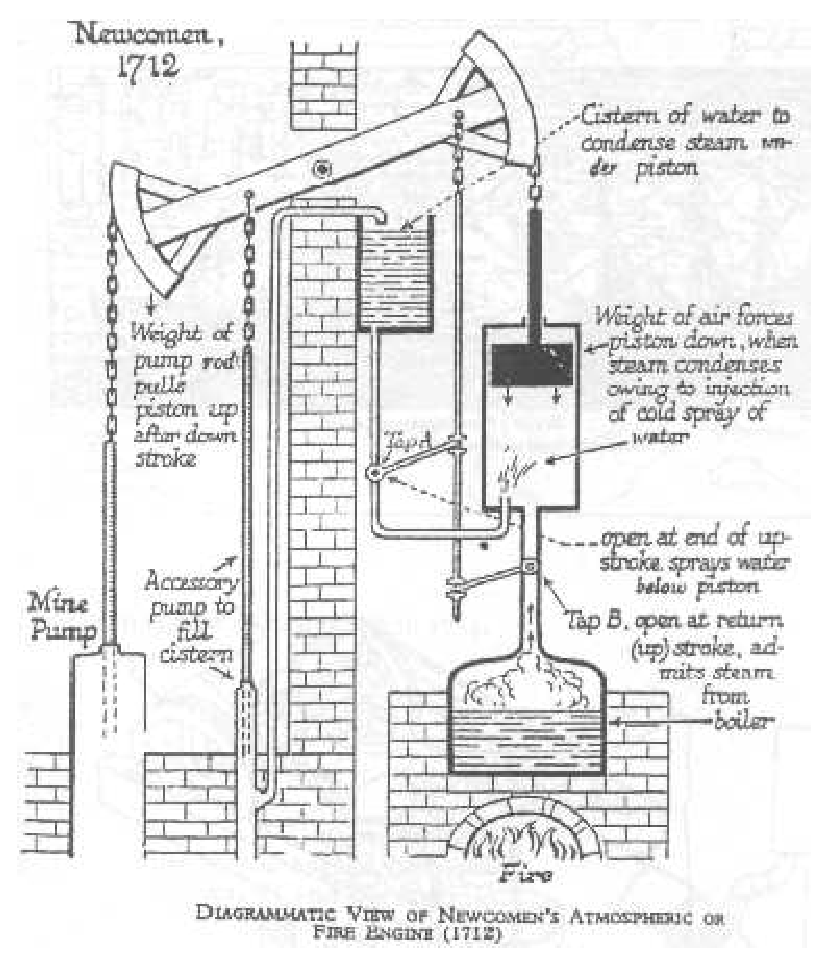
\includegraphics[height=10.0cm]{ambsthermopict/newcdiag.eps} 
} 
\caption{Converting heat to kinetic (mechanical) energy in 1712.}
\label{nse_people} 
\end{figure}  
A steam engine
is a particular form of a 
\emph{heat engine} converting heat to mechanical work in a thermodynamical
process. The modern \emph{combustion engine} in a car 
is a form of heat engine generating kinetic energy
from explosive burning of fuel.
 The efficiency of a heat engine is of 
prime importance, and can be studied by computational thermodynamics.
The necessary \emph{cooling} of a car engine represents 
a loss of energy which is not transformed into useful mechanical work.  

\section{Heat Pumps and Oil Crisis}

The \emph{heat pump} is replacing the increasingly expensive oil
for heating of houses. A heat pump converts low temperature heat energy
from the earth or the air to higher temperature useful heat energy, by
supplying the necessary conversion energy from electricity.
The efficiency is today typically around $2/3$, that is, for $1/3$
unit of electric energy, you get out 1 unit of useful heat energy. 
You can thus reduce your electrical bill by a factor of $3$ by
changing from full electrical heating of your house 
to heating by an efficient heat pump. Of course, it is of interest 
to seek to increase the efficieny even more. Can we reach $99\%$ 
efficiency, and if not why? We will address this question below.

\section{Refrigerators and Urban Civilization}

A \emph{refrigerator} is a form of heat pump taking heat from
the inside of the refrigerator and delivering it to the exterior at
higher temperature. 
The refrigerator is an absolute necessity of modern urban civilization.

The standard design builds on cycling a fluid alternating
between \emph{expansion/evaporation} to gas phase with temperature drop, and 
\emph{compression/condensation} to liquid phase with temperature increase,
with the cold gas in contact with the interior of the refrigerator 
and the warm liquid phase in contact with the exterior.
The cooling process with heat flowing from
cold to hot (contrary to its natural tendency to flow from hot to cold)
is thus maintained by an (electric) \emph{compressor} 
consuming energy.

\begin{figure}[bhpt] 
\centerline{ 
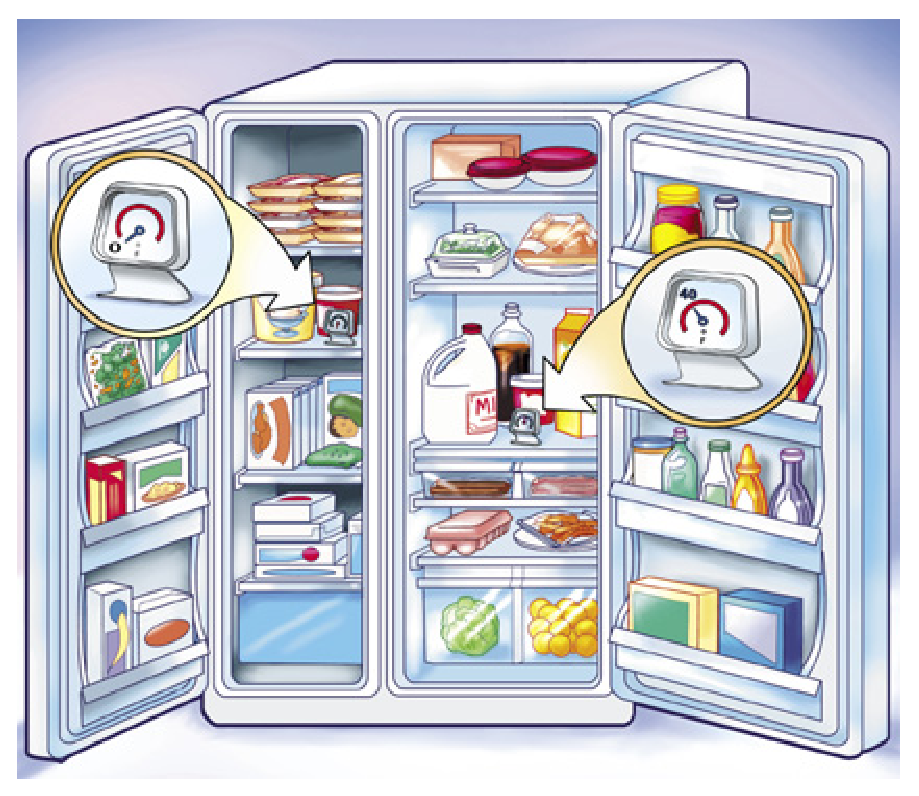
\includegraphics[height=6.0cm]{ambsthermopict/refrigerator.eps} 
} 
\caption{Inside a refrigerator: The principle of preservation of food.}
\label{nse_people} 
\end{figure}




The first design of an \emph{absorption refrigerator}, without compressor and
moving parts and thus silent,
was invented by the two young Swedish
engineering students Carl Munters and Baltzar von
Platen during their class in 
thermodynamics at the Royal Institute of Technology in 1922
(although they slept through the lectures working all night
on their invention).
This invention together with a vacuum cleaner
gave the impetus of the quick expansion of the Electrolux company.
The production of the Munters-Platen refrigerator has 
continued at Motala in Sweden uninterrupted
since 1925 with today a total of 10 million units being produced. 
We hope this book may be useful for young minds of today
for new inventions.


\section{Information and Communication}

\emph{Information theory} was created by Shannon \cite{shannon} in 
the 1940s borrowing the concept of \emph{entropy} from 
\emph{thermodynamics}, with the idea of measuring  
communication channel capacity requirements for different types of information.
Random information would then represent information with
maximal entropy, in principle requiring maximal capacity
(although random information would seem like useless information). 
 
Alternatively, one can view communication of information as a 
thermodynamic flow with the heat energy
representing loss or destruction of information during the communication.
More generally, not only creation but also destruction 
of information represent fundamental aspects of 
physical and biological processes.

\begin{figure}[bhpt] 
\centerline{ 
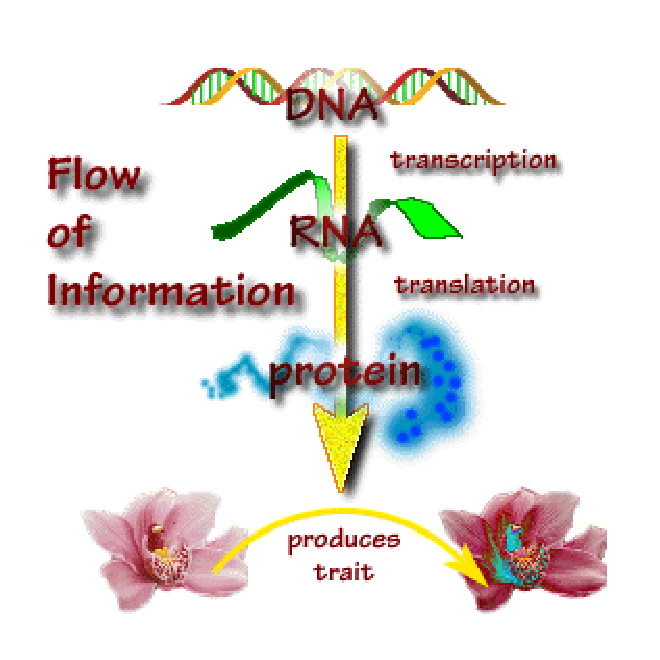
\includegraphics[height=6.0cm]{ambsthermopict/GPFlowInfo.eps} 
} 
\caption{Flow of information in a flower.}
\label{nse_people} 
\end{figure}



\section{Economy and Welfare}

One can also view an evolving economy as a 
thermodynamic flow process transforming resources into utilities.
In (a free) economy turbulent dissipation could be viewed as a measure
of necessary losses during the process, in the form of interest rates,
taxes, bribes, 
thefts, which cannot (fully) be avoided. The flow of the World economy 
represents a complex process of prime importance to all of us.
An economist with (some) understanding of the process can be raised to 
fame and fortune.  

\begin{figure}[bhpt] 
\centerline{ 
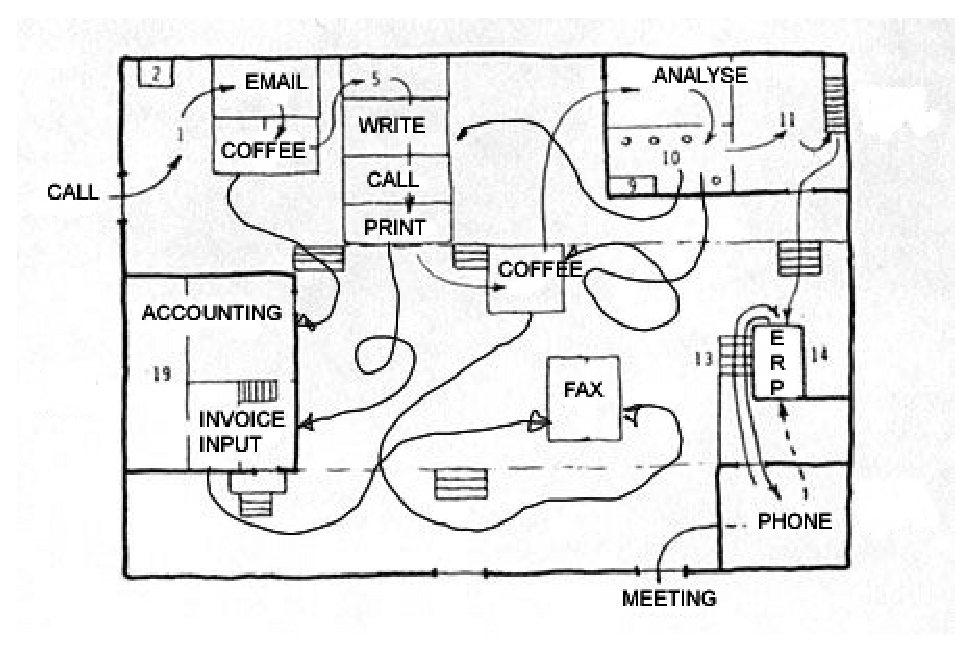
\includegraphics[height=6.0cm]{ambsthermopict/brainshopflow.eps} 
} 
\caption{Flow of information in an office of the last century.}
\label{nse_people} 
\end{figure}

\section{Emergence: A New Approach to Physics}

Ilya Prigogine received the Nobel Prize in Chemistry in 1977
for his work on \emph{non-equlibrium thermodynamics} proposing
a new (statistical) approach to the 2nd Law
allowing ordered structures to develop from non-ordered, see  
%\hyperref[ilyaworld]{Fig. \ref{ilyaworld}} and \ref{ilya}.
Fig. \ref{ilyaworld} and \ref{ilya}.
Even if Prigogine did not convince the physics
community at large, he at least showed the severe short-coming 
of the classical 2nd Law seemingly preventing order from
develping from chaos.

\emph{Emergence} is the process of complex pattern formation
from more basic constituent parts or ``particles'', that is the formation
of order out of chaos. Turbulence shows phenomena of both emergence
and featureless chaos, none of which can be understood by considering only
a single fluid particle, only by considering the interaction of many.
The (new) 2nd Law expresses a collective behavior of many 
fluid particles to form turbulent flow with an 
irreversible transfer of large scale kinetic energy to 
heat energy. Thus thermodynamics
naturally connects to the new approach to physics 
based on emergence, which is now
developing (emerging) 
with input from e.g. 1988 Nobel Laurate Robert Laughlin \cite{laughlin}, 
and which is
radically different from the \emph{reductionist} approach of elementary
particle physics completely dominating the scene since the 
birth of quantum mechanics in the beginning of the last century.

Since emergence concerns the interaction of many particles, analytical
methods fall short (which lies behind the reductionist
obsession with a single particle
hopefully allowing analytical mathematical description),
while computational methods open new possiblities of simulating
emergent and turbulent phenomena, as is shown in this book.


\begin{figure}[bhpt] 
\centerline{ 
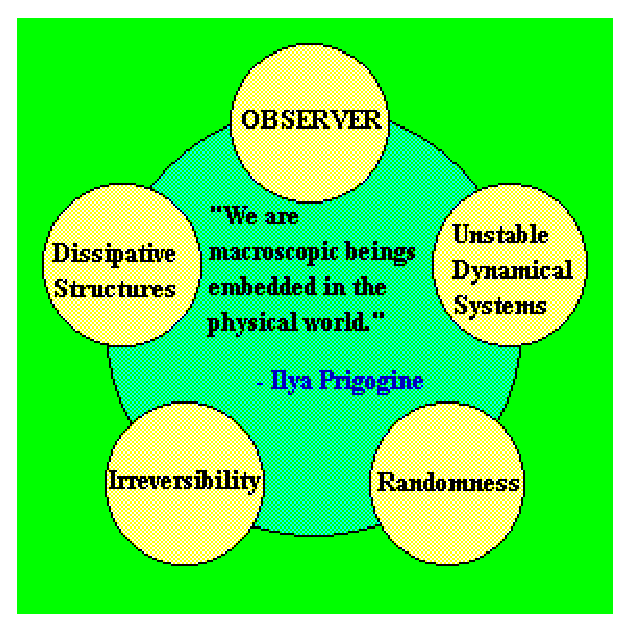
\includegraphics[height=8.0cm]{ambsthermopict/ilyaflow.eps} 
} 
\caption{The World according to Ilya Prigogine.}
\label{ilyaworld} 
\end{figure}\begin{figure}[bhpt] 
\centerline{ 
\includegraphics[height=8.0cm]{ambsthermopict/prigogine.eps} 
} 
\caption{Ilya Prigogine receiving the Nobel Prize in Chemistry
in 1977 from the hands of King Karl XVI Gustav.}
\label{ilya} 
\end{figure}

\section{The Battle between Growth and Decay}

We shall see that turbulent flow and thus thermodynamics (the World)  
can be viewed as a battle between a growth process of \emph{differentiation
by advection} and a decay process of \emph{mixing by diffusion} according
to:
\begin{itemize}
\item \emph{growth: increase difference-differentiate-separate: advection}
\item \emph{decay: decreasse difference--uniformize-mix: diffusion.}
\end{itemize} 
The classical 2nd Law captures the diffusion process with mixing
and decreasing difference. But it does not capture the 
advection process allowing increasing difference and separation,
which is a severe short-coming. The new 2nd Law captures
both processes. In the thermodynamics of Prigogine the two processes are
represented  by ``Unstable Dynamical Systems'' and ``Dissipative Structures'',
but Prigogine sticks to ``Randomness'', see Fig. \ref{ilyaworld}.


\section{Physics: Flow of Information: Computation}

The basic idea of this book 
is to view thermodynamics as a form of 
analog computation, which can be simulated by digital computation. 
Both analog physics and digital computation can be seen as  
flows of information reflecting the flow of mass, momentum and 
energy in a physical system and the flow of digits from input to output in the
execution of a subroutine of the computational code.

For a computer programmer the information flow is 
represented in the flow chart of a computer code, which
is essential for the understanding of the code. 
Likewise, a flow chart of the analog computation 
of a physical process can help the physicist 
to understanding.



 
\section{Thermodynamics as a ``Best of  Worlds''}

The above survey indicates that thermodynamics 
is a fundamental part of science and
technology and thus serves a very important role in our society.
Thermodynamics is maybe the scientific field closest to 
Leibniz' definition of a \emph{Best of Worlds}
as a world, which is richest in variation of ordered complex
structures or emergence, such as different forms of life and conscience,
while being governed by simplest possible principles or laws.



\small
\begin{quote}I say that I am strongly inclined to believe that heat is of 
the same kind, and that material things which make us hot and feel hot 
(such as we call by the general name \emph{fire} are a multitude of tiny 
corpuscles of such and such a shape, and moving at such and such a speed. 
When they meet our bodies, they penetrate them with their extreme subtlety, 
and the way they touch our substance as they pass through it is sensed by 
us as the affection we call ``heat''. 
It is pleasant or unpleasant in 
proportion to the number and speed of the particles as they prick and 
penetrate it. This penetration is pleasant if it is beneficial to our 
insensible vital functions, and unpleasant when it causes too much of a 
separation and dissolution of our substance. (Galieo in \emph{The Assayer}, 
1623)
\end{quote}
\normalsize





\chapter{Refrigerator and Heat Pump}\label{ch:refrig}

The Joule expansion of the previous chapter is the working stroke of both a
\emph{refrigerator} (harvesting the cooled left chamber) and a \emph{heat pump}
(harvesting the warmed right chamber): one and the same device, distinguished
only by which reservoir's heat exchange is counted as useful. Because RNS
resolves the dynamics, we can read their efficiency directly off the computed
fields rather than postulate it.

\section{A Computable Model}

An interactive realisation (\texttt{joule\_experiment\_cpu.html}, a
dependency-free vanilla-JS port of the original sketch) solves the 2D
compressible Navier--Stokes/RNS system
\[
\dot\rho+\nabla\cdot m=0,\qquad
\dot m+\nabla\cdot(mu)+\gamma\nabla e=\mu_{\mathrm{mom}}\,\Delta u,\qquad
\dot e+\nabla\cdot(eu)+\gamma e\,\nabla\cdot u=\mu_{\mathrm{mom}}\,|\nabla u|^2,
\]
with $p=\gamma e=\gamma\rho T$, $T=e/\rho$, $u=m/\rho$, on two chambers joined by a
channel: a dense, equally-warm left chamber ($\rho=e=10$, hence $T=1$) expanding
into a dilute right chamber ($\rho=e=1$). The last term in the energy equation is
the \emph{turbulent dissipation} $\mu_{\mathrm{mom}}|\nabla u|^2\ge 0$ --- the
irreversible return of the jet's kinetic energy to heat --- and crucially it uses
the \emph{same} coefficient $\mu_{\mathrm{mom}}$ as the momentum diffusion, so the
kinetic energy removed by viscosity reappears exactly as heat in the energy
equation and $K+E$ is conserved. A separate, much smaller coefficient
$\mu\ll\mu_{\mathrm{mom}}$ provides numerical stabilisation of $\rho$ and $e$
through Laplacian smoothing; it is not a physical dissipation and contributes
negligibly to the energy budget.

\section{Energy and Dissipation Bookkeeping}

The simulation tracks, at each instant, the kinetic energy
$K=\int\tfrac12\rho|u|^2\,dx$ and the internal energy $E=\int e\,dx$, with the
total $K+E$ conserved (Joule's null result for the \emph{whole} box), together
with the \emph{cumulative turbulent dissipation}
\begin{equation}\label{D_def}
D(t)=\int_0^t\!\!\int \mu_{\mathrm{mom}}\,|\nabla u|^2\,dx\,d\tau \;\;>\;0 ,
\end{equation}
which quantifies the irreversibility directly: it is positive by construction of
the discrete scheme and is \emph{the} 2nd Law for this model. There is no need
to introduce a statistical entropy $S$ or a relation $dS\ge 0$ --- the inequality
$D>0$ is the 2nd Law in its native, deterministic form, deriving from finite-
precision computation rather than postulated from probabilistic foundations.
$D$ accumulates wherever the velocity gradient is large: in the channel jet and
in the recompression against the far wall.

\section{Refrigerator and Heat Pump: Efficiency and the Cost of the Cycle}

A refrigerator runs \emph{cyclically}: each cycle the working gas must be
restored to its initial compressed state, so the relevant energy cost is the
work to restore the initial conditions. Its reversible (minimal) value is the
\emph{exergy} of the initial state; for the isothermal initial imbalance (both
chambers start at $T=T_0=1$) this is
\begin{equation}\label{exergyA0}
A_0=\gamma\int \rho\,\ln(\rho/\bar\rho)\,dx \;=\; D_\infty ,
\end{equation}
with $\bar\rho$ the mean density; the second equality states that the spontaneous
free expansion eventually destroys exactly this $A_0$ as accumulated turbulent
dissipation $D_\infty$ (\ref{D_def}). The cooling delivered is the heat removed from the cells
that drop below ambient,
\[
Q_{\mathrm{cold}}=\int_{T<T_0}\rho\,(T_0-T)\,dx ,
\]
and the coefficient of performance --- the buyer's figure of merit, cooling per
unit of work spent restoring the cycle --- is
\begin{equation}\label{copjoule}
\mathrm{COP}_{\mathrm R}=\frac{Q_{\mathrm{cold}}}{A_0}.
\end{equation}
The \emph{same} expansion is a \emph{heat pump} if instead we harvest the warmed
right chamber. Its useful output is the heat delivered to the hot side, which
over the full cycle is $Q_{\mathrm{hot}}=Q_{\mathrm{cold}}+A_0$ --- the cooling
moved up, plus the restore work $A_0$ rejected as heat during recompression ---
so
\[
\mathrm{COP}_{\mathrm{HP}}=\frac{Q_{\mathrm{cold}}+A_0}{A_0}=\mathrm{COP}_{\mathrm R}+1 .
\]
Refrigerator and heat pump are thus one device, the single Joule expansion,
distinguished only by which reservoir's heat exchange is counted as useful; in
the expansion phase alone the simulation shows $Q_{\mathrm{hot}}\approx
Q_{\mathrm{cold}}$ (pure redistribution at conserved total energy), the extra
$A_0$ entering on the hot side only during recompression.

Against the Carnot ceiling for the achieved lift,
$\mathrm{COP}_{\mathrm{Carnot}}=T_{\mathrm{cold}}/(T_{\mathrm{hot}}-T_{\mathrm{cold}})$,
the second-law efficiency $\eta=\mathrm{COP}_{\mathrm R}/\mathrm{COP}_{\mathrm{Carnot}}$ comes
out at only a few percent: the free expansion is a \emph{very poor} refrigerator,
destroying almost all of the available work $A_0$ as cumulative turbulent
dissipation $D$ while delivering only a sliver of cold. This is exactly why a
practical refrigerator does not free-expand but runs the recompression cycle of
the next chapter, recovering work and driving the lost-work $D$ down toward zero
(the Carnot limit). The same bookkeeping --- $A_0$, $Q_{\mathrm{cold}}$, $D$ ---
will let us assign an efficiency to any continuum-thermodynamic process,
including the thermodynamics of the living cell.


\chapter{The Piston-Cylinder: the Heat-Engine Problem}\label{ch:piston}

\small
\begin{quote}
The steam engine having furnished us with a means for converting heat
into motive power\ldots\ the idea of establishing theoretically some
fixed relation between a quantity of heat and the quantity of work
which it can possibly produce, from which relation conclusions
regarding the nature of heat itself may be deduced, naturally
presents itself.
\normalfont\hfill --- R.~Clausius, 1851.
\end{quote}
\normalsize

\section{The piston-cylinder as the heat-engine analogue of Joule}

The Joule experiment of Chapter~\ref{ch:joule} ran a pressure differential
between two fixed-wall chambers to mechanical equilibrium and observed
the residual temperature/density gap: a one-shot dissipation pattern with
no net work extracted. The companion foundational problem of
thermodynamics replaces the right-hand fixed wall of the Joule chamber
with a \emph{movable piston} and connects the piston to an external
mechanical load. Gas now does work on the load as it expands, and the
question becomes how much of the internal-energy decrease in the
gas reservoir reaches the load as work versus how much is irreversibly
dissipated as heat in the receiving region.

We treat two cases. The \emph{smooth} case is a single chamber filled
with hot dense gas, closed on three sides and with a piston as the
fourth wall. The gas expands quasi-statically against the load; in the
ideal limit of slow piston motion this approaches reversible expansion
with $\eta = W/\Delta U \to 1$. The \emph{Joule-coupled} case inserts a
constricted wall (a thin barrier with a small channel opening) between
the gas reservoir and the piston. The gas now jets through the
constriction, decelerates against the gas already in the receiving
region, and the recompression-and-turbulent-dissipation pattern of
Joule's experiment plays out --- but now with a piston on the far side
that captures whatever pressure survives. The efficiency drops below
the smooth limit by the amount of kinetic energy that turbulent
recompression converts back to heat rather than to useful pressure on
the piston. The two cases together display the fundamental engine
trade-off in the cleanest possible computational form.

\section{The smooth piston-cylinder}\label{sec:piston-smooth}

\paragraph{Configuration.}
A square domain $[0, 1]^2$ holds gas of initial density $\rho = 10$ and
internal energy $e = 10$ (so $p = \gamma e = 1.0$ with $\gamma = 0.1$)
to the left of a movable piston initially positioned at $x = 0.5$. To
the right of the piston lies an external region held at a fixed load
pressure $P_{\rm ext} = 0.5$. The top and bottom walls of the chamber
are zero-flux/free-slip, the left wall is closed, the right boundary
beyond the piston is the load.

\paragraph{Dynamics.}
Newton's second law for the piston, with $M$ the piston mass per unit
$y$-length and a friction coefficient $c$ for piston-rail damping, reads
\begin{equation}\label{eq:piston-newton}
M\,\frac{\rd v_p}{\rd t} = \int_{0}^{1}\!\bigl[\,p_{\rm gas}(x_p^-, y) - P_{\rm ext}\,\bigr]\,\rd y \;-\; c\,v_p,
\quad \frac{\rd x_p}{\rd t} = v_p,
\end{equation}
where $p_{\rm gas}(x_p^-, y) = \gamma\,e(x_p^-, y)$ is the local
gas pressure on the piston's gas-side face. The gas occupies the
domain $x \in [0, x_p)$ and evolves by the compressible
Navier--Stokes equations of Chapter~\ref{ch:joule}, with a no-slip
ghost at the piston face. Work delivered to the load per unit time is
\begin{equation}\label{eq:piston-power}
\dot W = P_{\rm ext} \cdot v_p \cdot \mathrm{Area},
\end{equation}
and the heat-engine efficiency is
\begin{equation}\label{eq:piston-eta}
\eta = \frac{W}{\Delta U} = \frac{\int_0^t \dot W\,\rd s}{U(0) - U(t)}.
\end{equation}

\paragraph{Behaviour and expected result.}
The smooth piston-cylinder is the cleanest computational instance of
quasi-static isobaric expansion. With slow piston motion (small $v_p$
compared with the acoustic speed $c_s = \sqrt{\gamma e/\rho}$ in the
gas), the gas expands without significant kinetic-energy generation;
the work-delivered counter and the heat-lost counter grow together;
and $\eta$ approaches the reversible limit. Faster piston motion
generates acoustic waves in the gas region that bounce between the
left wall and the piston face, with each acoustic round-trip a small
turbulent-dissipation loss; $\eta$ falls below 1 by an amount
proportional to the piston Mach number. The smooth case therefore
isolates the fundamental work-extraction mechanism, with irreversibility
present only as a small correction proportional to the piston speed.

The accompanying simulator \texttt{heat\_engine.html} (Appendix~A
Gallery) implements~\eqref{eq:piston-newton}--\eqref{eq:piston-eta} for
$N = 200$, $\gamma = 0.1$, $P_{\rm ext} = 0.5$, $M = 0.05$,
$c = 1.5$. The piston moves from $x_p = 0.5$ outward over $\sim 10\,$s
of wall-clock time, with $\eta$ reaching $\sim 0.7$--$0.9$ depending on
the piston-Mach-number regime.

\section{The Joule-coupled piston-cylinder}\label{sec:piston-joule}

\paragraph{Configuration.}
The same square domain holds a high-pressure gas reservoir on the left
($i < I_w$ in grid units, $\rho = 10$, $e = 10$), a thin barrier wall at
$i \in [I_w, I_w + w_{\rm wall}]$ with a small channel opening at
$j \in [J_0, J_1]$, a receiving region between the barrier and the
piston ($I_w + w_{\rm wall} < i < x_p$, initially $\rho = 1$, $e = 1$),
and the movable piston at $i = x_p$. The external load is held at
$P_{\rm ext} = 0.1$, matching the initial pressure in the receiving
region so the piston starts in mechanical equilibrium and is pushed
outward only after the channel inflow has compressed the receiving
gas.

\paragraph{Dynamics.}
The piston obeys the same Newton's-law update~\eqref{eq:piston-newton}
with $p_{\rm gas}$ now the local pressure in the receiving region
just to the left of the piston face. The gas equations are unchanged;
the barrier is a frozen no-slip wall except in the channel opening,
where gas can flow freely. The barrier presents the classical
Joule constriction to the gas: the high reservoir pressure drives a
jet through the channel, the jet decelerates in the receiving region,
and the kinetic-energy-to-heat conversion of turbulent
recompression dissipates a fraction of the released internal energy
into heat in the receiving region rather than into useful pressure
against the piston.

\paragraph{Two energy accounts.}
The 1st Law of thermodynamics for this system says
\begin{equation}\label{eq:piston-1st-law}
\underbrace{\Delta U_{\rm reservoir}}_{\text{heat lost from hot side}}
\;=\;
\underbrace{W}_{\text{useful work}}
\;+\;
\underbrace{\Delta U_{\rm receiving}}_{\text{heat dumped in cold side}}
\;+\;
\underbrace{K_{\rm channel}}_{\text{kinetic energy in flight}}.
\end{equation}
The transient $K_{\rm channel}$ goes to zero at long times as the gas
equilibrates; in the steady state, all of the released $\Delta U_{\rm reservoir}$
ends up either as work $W$ or as $\Delta U_{\rm receiving}$ (waste heat).
The 2nd Law tells us which split is realised: the size of
$\Delta U_{\rm receiving}$ is set by the dynamic
turbulent-dissipation pattern in the recompression process, exactly
as in the Joule experiment of Chapter~\ref{ch:joule}. The engine
efficiency follows as
\begin{equation}\label{eq:piston-eta-joule}
\eta \;=\; \frac{W}{\Delta U_{\rm reservoir}} \;=\; 1 - \frac{\Delta U_{\rm receiving}}{\Delta U_{\rm reservoir}}\;-\;\frac{K_{\rm channel}}{\Delta U_{\rm reservoir}},
\end{equation}
and in the steady state $\eta < 1$ by exactly the fraction of energy
that the Joule turbulent-recompression channel dissipates as heat.

\paragraph{One-shot versus sustained operation.}
With the left wall closed (finite reservoir), the simulation runs as a
\emph{one-shot} cycle: the reservoir depletes, the piston receives a
brief impulsive load from the channel-driven shock and a slower
follow-on pressure as the gas equilibrates, and the engine extracts a
single power stroke of work. This is the elementary unit of a
reciprocating closed-cycle heat engine (Otto, Diesel, Stirling).
With the left wall replaced by a Dirichlet inflow boundary maintaining
the reservoir state at $\rho = 10$, $e = 10$ indefinitely, the
simulation runs as a \emph{sustained} cycle: gas keeps jetting through
the channel, the piston reaches a quasi-steady velocity, and power is
delivered continuously. This is the elementary unit of an open-cycle
flow engine (gas turbine, jet engine). The two operating modes are
selected in the simulator \texttt{heat\_engine\_with\_channel.html}
(Appendix~A) by the choice of left-wall boundary condition: zero-gradient
mirror for one-shot, Dirichlet inflow for sustained.

\section{Joule and the piston as duals}\label{sec:joule-piston-duals}

The two central problems are duals of each other:
\begin{itemize}
\item \textbf{Joule's experiment} (Chapter~\ref{ch:joule}) lets the
expansion-and-recompression dynamics run to mechanical equilibrium
with no work extracted, leaving a residual temperature/density gap
between the chambers that is the dynamic-dissipation signature. With
external work added cyclically by a compressor, this becomes a
\textbf{refrigerator}: the residual asymmetry is held against
diffusive relaxation by continuously re-energising the gas, and the
asymmetric temperature gradient is exploited to draw heat from cold
side and dump it to hot side.

\item \textbf{The piston-cylinder} (this chapter) lets the same
expansion-and-recompression dynamics run with a movable wall as the
right boundary, extracting useful work to an external load. With
external heat added cyclically by a hot reservoir at the inflow, this
becomes a \textbf{heat engine}: the released internal energy is split
between work delivered to the load and waste heat dumped to a cold
side, with the efficiency $\eta$ set by the same turbulent-dissipation
fraction.
\end{itemize}
Both problems are governed by the same compressible
Navier--Stokes equations, the same RNS finite-element discretisation,
and the same 2nd-Law-as-finite-precision reading of irreversibility.
The framework of this book treats them as the two foundational
single-shot configurations of which all cyclic engines, pumps,
refrigerators, and heat-recovery devices of Vol VI Applications are
built; everything else in thermodynamics is either a cyclic repetition
of these or a multi-stage combination of them.

\section{What this chapter establishes}

For the rest of the book the reader should hold three observations
from this chapter and the previous one together:
\begin{enumerate}
\item Pressure-driven flow through a constriction converts internal
energy into kinetic energy; recompression on the receiving side
converts a fraction of that kinetic energy back into heat
irreversibly; the size of that fraction is the dynamic content of the
2nd Law and is what classical equilibrium thermodynamics cannot
predict.

\item A piston in the receiving region intercepts a fraction of the
arriving pressure as useful work; the larger that fraction, the
smaller the recompression dissipation, the higher the engine
efficiency. The efficiency is bounded above by the reversible smooth-
expansion limit, and the irreversibility cost is the dynamical content
of the heat-engine inequality $\eta \le 1$.

\item Both the refrigerator and the heat engine are cyclic devices
built from a single foundational dynamic process: the
expansion-through-a-channel-followed-by-turbulent-recompression cycle.
Refrigerators run it as the heat-pumping cycle with work input;
heat engines run it as the work-output cycle with heat input. The
same simulation infrastructure produces both.
\end{enumerate}



\chapter{Information}



\small
\begin{quote} The fundamental problem of communication is that of reproducing
at one point either exactly or approximately a message selected
at another point. (Shannon in \cite{shannon}, 1948)
\end{quote}

\begin{quote} You should call it entropy for two reasons; in the first
place your uncertainty function has been used in statistical mechanics
under that name, so it already has a name. In the second place, and more
important, no one knows what entropy really is, so in a debate you
will always have an advantage. (von Neumann to Shannon)
\end{quote}
\normalsize

\section{Introduction}

\emph{Information theory} was created by Shannon \cite{shannon} in 
the 1940s borrowing the concept of 
entropy from thermodynamics. 
%In \cite{ambsflow}
%we presented a new foundation of thermodynamics based the \emph{1st Law of 
%thermodynamics} stating conservation of mass. momentum and energy,
%combined with a certain form of \emph{finite precision 
%computation}. In the new foundation the \emph{2nd Law of thermodynamics} is
%expressed without using the concept of entropy and 
%is a consequence of the 1st Law combined with finite precision computation.
We now explore if the new foundation 
of thermodynamics presented may open to a new approach 
to information theory.  
We thus consider a model of \emph{information flow} in the form
of the Euler equations for a variable density incompressible fluid 
flow with the distribution in space of \emph{mass density}  
representing information like a message, image or movie, 
which is being transported 
or \emph{communicated} from one location to another by the fluid flow.
The key question is what aspects of the 
information which can be communicated to what precision. 
We expect to see fine details of an image being 
distorted or destroyed by the communication, while
gross features may remain unaltered. We introduce a measure of 
\emph{irrecoverable loss of information}, which couples to
increase of entropy in the classical setting,
which corresponds to information which cannot be retrieved. 
We thus distinguish between 
\emph{recoverable information}, which can be recovered from a 
distorted image by some form of image processing, and
\emph{irrecoverable information} which cannot be recovered 
by image processing. 

\section{Entropy vs Loss of Information}

In Shannon's information theory the notion of entropy
is used to measure the randomness or complexity
of the information to be communicated, with random
complex information requiring more work to communicate than
organized simple information. Shannon's entropy thus is
a measure of the work to communicate certain information,
assuming that the communication itself does not distort
the information. In this setting information is
coded into a digital representation, which is communicated without loss
of any digits and then is decoded after reception. 
The main question then concerns the number
of digits required to represent the information, which directly couples
to the work of accurate communication of the digits.
In Shannon's theory the digital coding in general introduces a certain 
loss of information, with more loss for complex information,
while the communication of the digital
representation is assumed to be without loss. Shannon's entropy
thus may be viewed as a measure of loss of information arising
from the digital representation but not from the communication. 

Our notion of entropy is a bit different
and measures the \emph{total loss of information}
taking into account not only the loss from digital representation, but
also from the communication process itself. 
In our setting, the digital representation of the information
as a mass density, is a finite element approximation on a mesh
of certain mesh size $h$, which can
be viewed as generalized Fourier or wavelet representation,
and the communication is realized through a finite element
solution of the Euler equations. The mesh size $h$ directly
couples to the work required for the communication.

The main aspects influencing the
total loss of information, and thus the error in the communication,
relate to (a) the complexity of the information and (b) the
complexity of the communication process, where (b) can be viewed as
a measure of the distortion from the communication process. We 
identify the following basic cases:
\begin{itemize}
\item[(i)] simple information and simple communication,
\item[(ii)] complex information and simple communication,
\item[(iii)] simple information and complex communication,
\item[(iv)] complex information and complex communication.
\end{itemize}
We will see that in (i) the loss of information typically is small,
in case (ii) and (iii) it is of medium size, and in case (iv) it is large.
We will see that (i) requires little work ($h$ is not small), 
(ii) and (iii) require medium work
and (iv) large work ($h$ small), for the same accuracy. 
We shall see that if the communication is partly \emph{turbulent}, 
which is the generic case, then the loss
of information cannot be made arbitrarily small 
by decreasing $h$, relecting that the 
turbulent dissipation has a non-zero limit as $h$ tends to zero.  
 



 

\section{A Model Problem}

 
As a simple model of communication, we consider the following
1d transport equation:
\begin{equation}\label{convection}
\begin{split}
\dot\rho + \rho '=&0\quad \mbox{for } 0<x<1\, ,0<t\le 2,\\
\rho (x,0)=&0 \quad \mbox{for } 0<x<1\,
\end{split} 
\end{equation}
where $\dot\rho =\frac{\partial \rho}{\partial t}$, 
$\rho '=\frac{\partial \rho}{\partial x}$, and
$\rho (0,t)=\rho^-(t)$ with $0\le t\le 1$  
represents an input signal and $\rho^+(t)=\rho (1,t)$
with $1\le t\le 2$ the corresponding output signal. Since the solution to the 
convection equation is given by $\rho (x,t)=\rho (0,t-x)$ for
$t\ge x$, we simply have $\rho^+(t)=\rho (1,t)=\rho (0,t-1)=\rho^-(t-1)$ for $1\le t\le 2$, that is, 
the output signal is equal to the input signal with a unit time delay.

Let now $\rho_h$ be a finite element computational solution of the convection
problem representing a realization of the communication from input to
output with a certain imprecision due to the numerics. 
More precisely, let $\rho_h\in V_h$ be
a cG(1)-solution determined by
\begin{equation}\label{g2}
((\dot\rho_h+\rho_h',v))+(\rho (0,\cdot )-\rho^-,v(0,\cdot ))+((h\rho_h',v'))=0,
\quad\mbox{for all } v\in V_h,
\end{equation}
where $V_h$ is the set of continuous piecewise linear functions
on a space-time mesh of $Q=[0,1]\times [0,2]$ with mesh size $h$, $((v,w))=\int_Qvw\, dxdt$
and $(v,w)=\int_0^1vw\, dx$.  Here, the first two terms come out of
Galerkin's cG(1)-method and boil down to a centered difference
scheme on a regular mesh and the the third term is a stabilizing
artifical viscosity
term. More generally, we may apply the RNS method
with a residual-based artificial viscosity. 

We observe observe the reverse  
communication process taking $\rho^+$ to $\rho^-$, would
read: Find $\rho\in V_h$ such that
\[
((v,-\dot\rho_h-\rho_h'))+(\rho (1,\cdot )-\rho^+,v(1,\cdot ))
+((h\rho_h',v'))=0,
\quad\mbox{for all } v\in V_h,
\]
where $(v,w)=\int_1^2vw\, dx$. This means that neglecting the 
viscous terms, we could retrieve $\rho_h^-$ exactly from $\rho^+_h$ by
time stepping backwards in time. In contrast, we cannot ``undo''  the
effect of the viscous term in a process from $\rho_h^-$ to $\rho_h^+$,
since time stepping backwards with the artificial viscosity
present would just add more diffusion to the
process.

To study the resulting output error in the communication from
$\rho^-$ to $\rho^+$,  
let $\psi (t)$ with $1\le t\le 2$ be a given weight function,
and let $\varphi (x,t)$ solve the dual problem
\begin{equation}
\begin{split}
-\dot\varphi - \varphi '=&0\quad \mbox{for } 0<x<1\, ,0<t\le 2,\\
\varphi (x,2)=&0 \quad \mbox{for } 0<x<1,\\
\varphi (1,t)=&\psi (t) \quad \mbox{for } 1<t<2.
\end{split} 
\end{equation}
Multiplying the dual equation by $e=\rho -\rho_h$, integrating by parts
and using (\ref{g2}) assuming $\rho_h(0,\cdot )=\rho^-$, we obtain 
the following error representation:
\[
E_h\equiv \int_1^2(\rho^+-\rho_h(1,\cdot ))\psi dt=\int_1^2e(1,t)\psi (t)\, dt=((R(\rho_h),\varphi -\varphi_h))
+((h\rho_h' ,\varphi_h')),
\]
where $R(v)=\dot v+v'$, and $\varphi_h\in V_h$ is a finite element 
approximation $\varphi$. 

It is now natural to define $I=(R(\rho_h),\varphi -\varphi_h))$ 
to represent a \emph{recoverable} error, and 
$II=((h\rho_h' ,\varphi_h'))$ an \emph{irrecoverable} error.
In particular, 
choosing $\varphi_h$ to be a cG(1)-approximation,
we can make the I vanish, which may be viewed as 
retrieving $\rho^-$ by backwards time stepping. With this motivation
we now focus on the irrecoverable part $II$ of the error, neglecting
here the recoverable part $I$, and thus consider the error representation
\begin{equation}\label{error}
E_h\approx ((h\rho_h' ,\varphi_h')).
\end{equation}


We can now rephraze the above basic cases as follows: 
(i) $\rho_h$ and $\varphi_h$ smooth,
(ii) $\rho_h$ smooth and $\varphi_h$ non-smooth , (iii) 
$\rho_h$ non-smooth and $\varphi_h$ smooth, and (iv)
$\rho_h$ non-smooth and $\varphi_h$ non-smooth. We will then typically have
in case (i): $E_h\approx h$, in cases (ii) and (iii): $E_h\approx\sqrt{h}$
and in case (iv): $E_h\approx 1$. 
We may refer to (i) and (ii) as laminar cases and (iii) and (iv)
as turbulent cases. With a smooth $\varphi$, we measure 
the output error in a weak mean value sense, and with a non-smooth
$\varphi_h$ we measure the error in a more pointwise sense. 
We see that in the case of non-smooth $\rho_h$, 
only mean-value outputs can be meaningful.

Viewing entropy as a measure of loss of information, we may say
that (i) has small entropy production or little loss of information, 
(ii) and (iii) has medium entropy production and loss of information
while (iv) has massive entropy production and loss of information.

   
\section{Simulations in Model Problem}
 


 




\section{Euler's Equations}

We now generalize to the Euler equations for a variable density 
incompressible fluid
over a time interval $I=(0,T)$,
in a cylinder $\Omega =\{x=(x_1,x_2,x_3)=(x_1,\bar x): 0\le x_1\le L,\, \vert\bar x\vert\le R\}$
of length $L$ and radius $R$, with boundary $\Gamma$ with outward unit
normal $n$,  take the form: 
Find the \emph{density} $\rho (x,t)$, the 
\emph{flow velocity} $u(x,t)$ and \emph{pressure} $p(x,t)$, such that
\begin{equation}\label{euler}
\begin{split}
\dot\rho + \nabla\cdot (\rho u)&=0\quad \mbox{in } \Omega\times I,\\
\dot u+u\cdot\nabla u +\frac{\nabla p}{\rho}&=0\quad \mbox{in } \Omega\times I,\\
\nabla\cdot u&=0\quad \mbox{in } \Omega\times I,\\
u\cdot n&=u^-\quad \mbox{on } \Gamma^-\times I,\\ 
\rho &=\rho^-\quad \mbox{on } \Gamma^-\times I,\\ 
\rho (\cdot ,0)&=\rho^0, \, u(\cdot ,0)=u^0\quad \mbox{in } \Omega,\\ 
\end{split}
\end{equation}
where the fluid enters $\Omega$ through 
$\Gamma^- =\{x\in\Gamma :x_1=0\}$ with a given
inflow velocity $u\cdot n=g<0$ and
leaves through $\Gamma^+ =\{x\in\Gamma :x_1=L\}$ with
$u\cdot n>0$, and
$u\cdot n=0$ on the remaining (inpenetrable) part of the boundary.
Here $\rho (0,\cdot, \cdot )=\rho^-$ represents a given
input signal, or rather movie, consisting of 
a sequence of time dependent 2d images $\rho^-(\cdot ,t)$
with $t\in I$, defined on the cylinder cross section 
$\omega =\{\bar x:\vert\bar x\vert\le R\}$,  which is transported 
by the flow through the channel
to an output movie $\rho^+(\cdot ,t)=\rho (L,\cdot ,t)$ for $t$ in
a relevant interval.
The communication thus concerns the transformation of $\rho^-$ to
$\rho^+$. The basic problem concerns the \emph{distortion}
$d=\rho^+-\rho^-$, which measures the \emph{accuracy} of the
communication.


It is natural to assume that $\rho =\bar\rho +\tilde\rho$ 
where $\bar\rho$ is a constant given ``background'' and $\tilde\rho$
contains the information of interest. 
Replacing $\rho$ by $\bar\rho$ the second equation (momentum equation)
takes the form 
$\dot u+u\cdot\nabla u +\nabla\bar p=0$ with the modified pressure
$\bar p=p/\bar\rho$. This decouples $\rho$ from the last two equations,
which determine $(u,\bar p)$ as a solution to the (unit density)
incompressible Euler equations. In this case, $\rho $ thus can be 
determined from the first equation alone, which with $(u,\bar p)$ given 
is a linear convection equation.
For simplicity we consider this decoupled situation below, in which
the image itself is not influencing the flow, and thus is 
transported ``passively''.

The solution $(u,\bar p)$ to the (unit density) incompressible Euler 
equations in general is (partly) \emph{turbulent} with a complex 
flow velocity $u$, and thus the image 
$\rho (\cdot ,t)$ in general is convected in a (partly) complex 
convection field with a corresponding distortion. 
For short time also a \emph{laminar}
smooth flow velocity $u$ is possible. Thus the image can be
convected by a laminar or turbulent flow velocity, with vastly different
distortion effects. 

\section{Finite Precision Euler Solution: RNS}

We solve the Euler equations (\ref{euler}) using 
as above a stabilized cG(1)-method
on a finite element mesh in space-time
with mesh size $h(x,t)$, and denote the finite element solution  
by $\hat u_h=(\rho_h,u_h,p_h)$ with output $\rho_h^+$.
We will compare with a non-distorted output $\rho^+=\rho^-$
convected by a constant velocity field $\bar u(x,t)=(\bar u_1,0,0)$, 
where $\bar u_1$ is a representative inflow velocity. We will 
thus as a measure of the distortion, use the mean value 
\begin{equation}\label{E}
E_h=\int_\omega (\rho^--\rho_h^+)\psi \, d\bar x\, dt.
\end{equation}
where $\psi (\bar x,t)$ is a weight function. 



    


\section{Error Estimation by Duality}

As in the model problem, we may assume that
(see \cite{ambsflow} for details)
\[
E_h\approx ((h\nabla \rho_h,\nabla \varphi_h )),
\]
where $((v,w))=\int_0^T\int_\Omega vw\, dx\, dt$, and
$\varphi_h$ is an approximate solution of the dual problem
\[
\begin{split}
-\dot\varphi -u_h\cdot\nabla \varphi &=0\quad \mbox{in } \Omega\times I,\\\\
\varphi (L,\cdot ,\cdot)&=\psi \quad \mbox{in } \omega\times I,\\ ,\\
\varphi (\cdot ,T)&=0 \quad \mbox{in } \Omega,\\,
\end{split}
\]


\section{Laminar and Turbulent Communication}
As in the model problem, $E_h$ depends both on 
$\nabla\rho_h$ and $\nabla\varphi_h $.
If $u$ is turbulent, then $E_h$ may be small if $\psi$ is smooth with
large support, corresponding to a gross feature of interest.
If $u$ is laminar, then $E_h$ may be small also 
for a small feature of interest.

\section{The 2nd Law}

The basic energy balance for $\rho_h$ reflecting the structure
of the stabilized cG(1) method, reads:
\[
\int_{I^+}\int_\omega\rho_h (L,\bar x,t)^2\, dx\, dt+
D(\rho_h)=
\int_{I^-}\int_\omega\rho_h (0,\bar x,t)^2\, dx\, dt 
\]
where
\[
D(u_h;\rho_h) =\int_0^T\int_\Omega h\vert\nabla\rho_h\vert^2\, dx\, dt,
\]
and  $I^-$ and $I^+$ are relevant time intervals for input and output,
respectively.
As above, $D(u_h;\rho_h)$ represents 
an \emph{irrecoverable loss of information}. Reversing the
process letting $\rho_h$ convect backwards in time starting from
$\rho_h(\cdot ,T)$, we have an analogous energy balance
with a new dissipation term of positive sign, showing that
the initial data $\rho (\cdot ,0)$ cannot be fully recovered.
 

\section{Dissipation of Information}
As a rough measure of the amount of irrecoverable information  
we may use the \emph{total dissipation of information}:
\[
D_h=\int_0^T\int_\Omega h\vert\nabla\rho_h\vert^2\, dx\, dt.
\]
 


\section{Simulations}


We consider communication in cylindrical
channels of different length.
If the channel is short 
enough, then the flow may stay laminar all along the channel and the
image suffer little distortion, while if the flow gets turbulent, then
the image may get more distorted. Because of boundary layer effects
the distortion will usually be bigger close to the boundary.

We also study the effects of different obstructions in the channel
perturbing the flow, modeling a communication system with bottle-necks.

\begin{figure}[bhpt] 
\centerline{ 
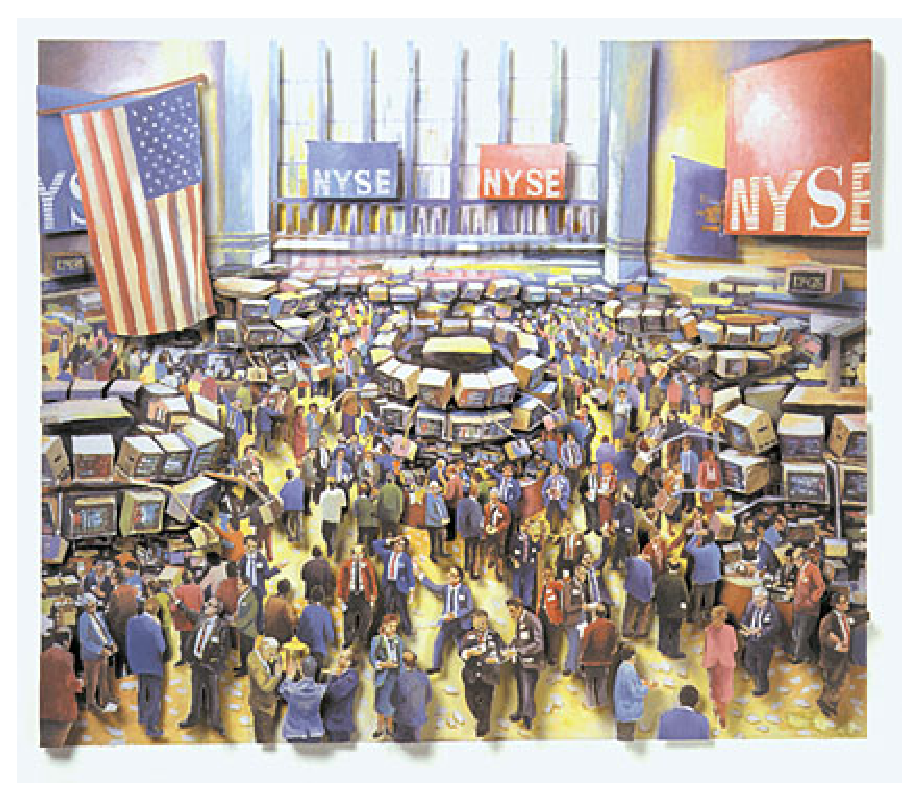
\includegraphics[height=4cm]{ambsthermopict/me-NYSE.eps} 
} 
\caption{Flow of information at New York Stock Exchange}
\label{stockexchange} 
\end{figure}

\chapter{Traffic Flow}

\small
\begin{quote}
I think the idea of getting out of a traffic jam and getting 
out of work each week and going and doing all this stuff would 
be really exhausting.(Paul McCarthy)
\end{quote}
\normalsize


\section{A Model of Traffic Flow}

We return to the simple traffic model which we considered above as
a variant of Burgers equation: Find the density $\rho (x,t)$ and 
the velocity $u(x,t)$ such that
\begin{equation}\label{traffic}
\begin{split}
\dot\rho+(u\rho )'&=0\quad\mbox{for } x\in\bbR ,\, t>0,\\
\rho (x,0)&=\rho^0(x)\quad\mbox{for } x\in\bbR ,
\end{split}
\end{equation}
combined with the constitutive law $u=(1-\rho )$, assuming
$0\le\rho^(x)\le 1$ for $x\in\bbR$.

\section{Shocks and Congestions}

We have seen that a shock corresponds to
the abrupt changes of density and velocity encountered
when the end of que of packed cars at rest 
is propagating in the opposite direction to the
direction of the traffic.
 

\section{Rarefactions and Traffic Lights}

A rarefaction solution corresponds to the situation when
at a traffic light turning green, the cars gradually 
accelerate one after the other. A nonphysical shock solution
corresponds to the familiar situation when the driver
in the first car at the traffic light, does not notice the light turning
green, with the instability of this situation being illustrated 
by the fact that a slight ``honk'' usually will alert the driver
to get going and allowing the rarefaction to develop. Instead of a honk
a little bit of viscosity will get the car going.

\begin{figure}[bhpt] 
\centerline{ 
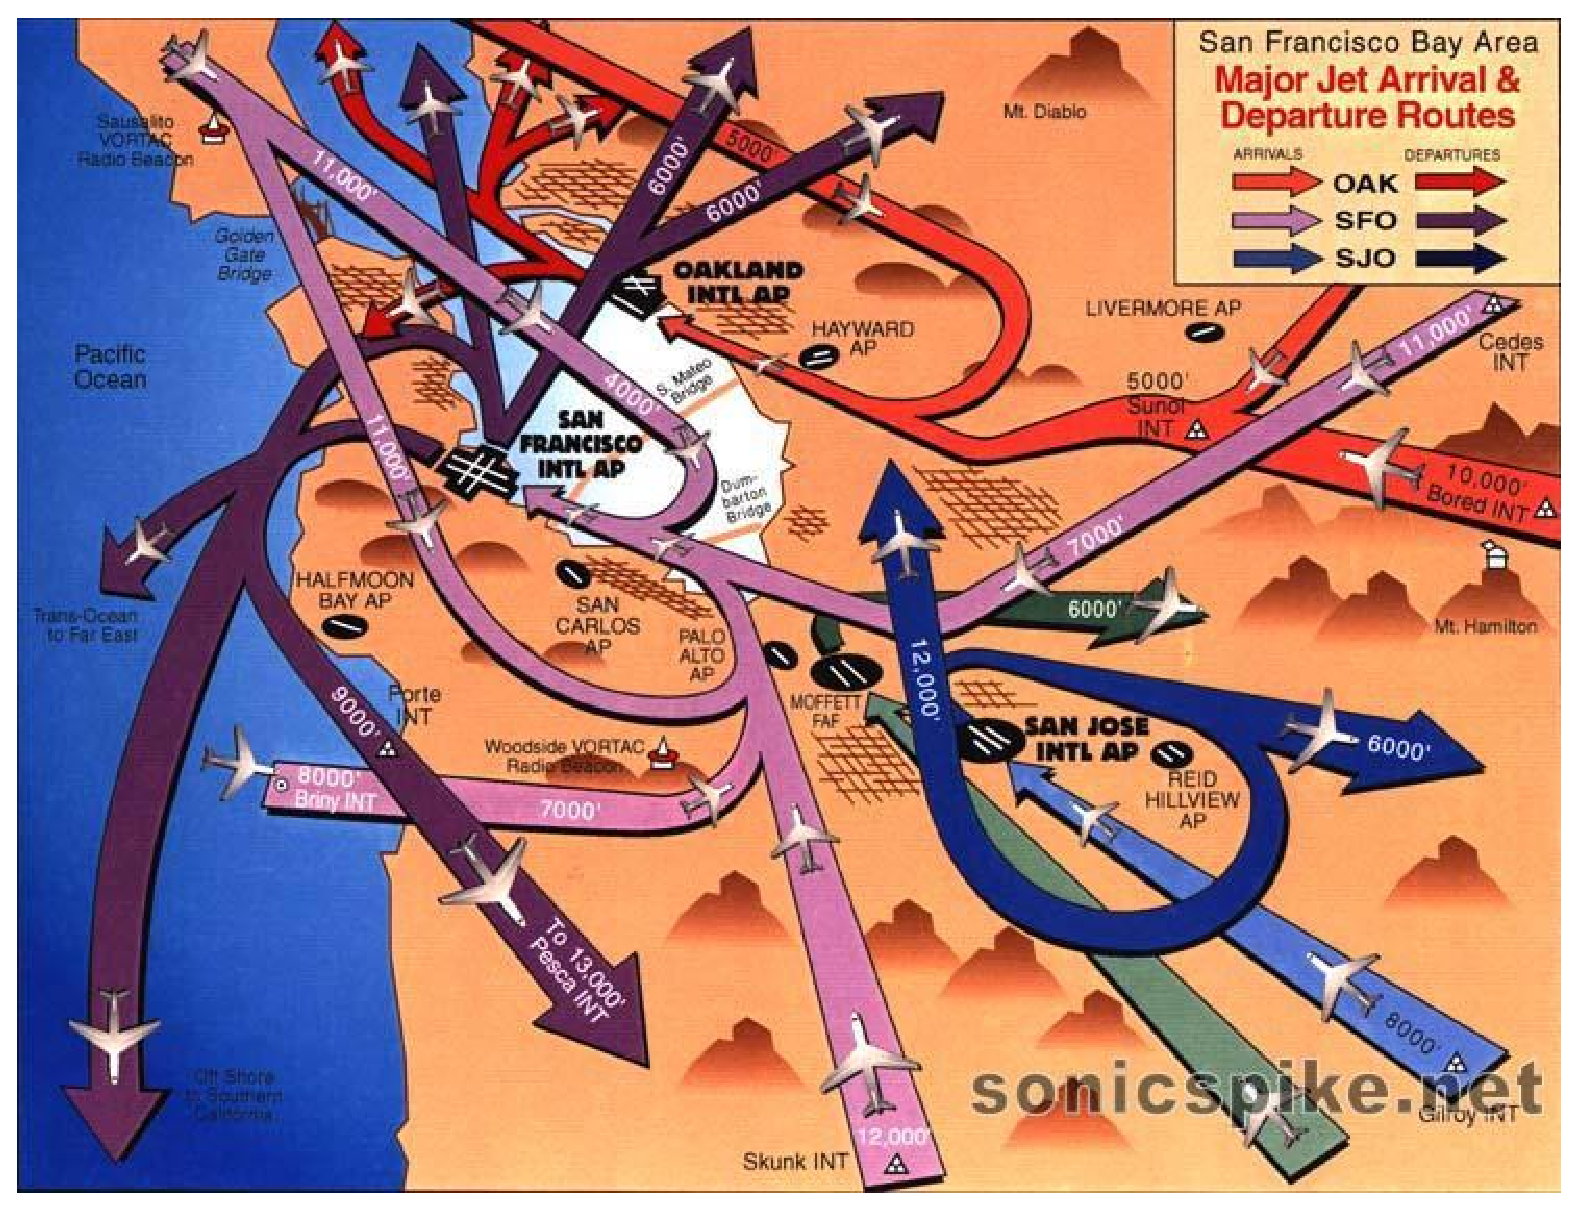
\includegraphics[height=8cm]{ambsthermopict/tfcflow-west.eps} 
} 
\caption{Traffic flow in the Bay Area}
\label{traffic} 
\end{figure} 


\chapter{Economy}

\small
\begin{quote}
    As every individual, therefore, endeavours as much as he can both to employ his capital in the support of domestic industry, and so to direct that industry that its produce may be of the greatest value; every individual necessarily labours to render the annual value of society as great as he can. He generally, indeed, neither intends to promote the public interest, nor knows how much he is promoting it. By preferring the support of domestic to that of foreign industry, he intends only his own security; and by directing that industry in such a manner as its produce may be of the greatest value, he intends only his own gain, and he is in this, as in many other cases, led by an invisible hand to promote an end which was no part of his intention. Nor is it always the worse for the society that it was no part of it. By pursuing his own interest he frequently promotes that of society more effectually than when he really intends to promote it. I have never known much good done by those who affected to trade for the public good. It is an affectation, indeed, not very common among merchants, and very few words need be employed in dissuading them from it. (Adam Smith)
\end{quote}
\normalsize
\section{A Flow Model}
We model an economy as a form of of reactive flow in a network.



% --- Part III openings (stubs) ---

\chapter{Biology: RNS with Metabolism}

\begin{quote}\itshape
A living cell sustains itself far from equilibrium by a continuous turnover
of matter and energy --- intake of fuel, oxidation in mitochondria, export
of waste heat. At the level of continuum mechanics this is a reacting,
diffusing, dissipating flow on a complex internal geometry: RNS with
metabolism. Glycolysis and the citric acid cycle deliver chemical free
energy at a controlled rate; ATP turnover couples that energy to mechanical
work in muscle and ion-pumping work across membranes; the by-products
diffuse out as low-grade heat. Schr\"odinger's ``negative entropy fed upon
by the organism'' is, in the RNS reading, simply the maintained gradient
that the organism must keep open to avoid the equilibration to which the
ambient dissipation would otherwise drive it. A companion browser
simulation \texttt{cell\_metabolism\_cpu.html} is forthcoming.
\end{quote}

\chapter{Process Industry: RNS with Unit Operations}

\begin{quote}\itshape
The chemical and process industry --- distillation columns, reactors,
heat exchangers, separators, fluidised beds, combustion chambers ---
realises ThermoDynamics with explicit engineering constraints: throughput,
selectivity, energy integration, environmental footprint. Each unit
operation is a controlled continuum flow with dissipation and (often)
chemical reaction; the plant as a whole is a network of such units coupled
by streams and heat-recovery loops. The RNS apparatus of this volume --- a
compressible reacting flow with positive dissipation $D > 0$ resolved at
finite precision --- is the same apparatus that the discipline of process
systems engineering applies under names like CFD-coupled flowsheet
simulation, pinch analysis, and exergy accounting. A companion sequence
of unit-operation simulations is forthcoming.
\end{quote}

\chapter{Climate: RNS with Radiation and the Hydrologic Cycle}

\begin{quote}\itshape
The Earth's atmosphere is a thin, rotating, stratified compressible flow
driven by an equator-to-pole insolation gradient, with phase change of
water as its dominant internal energy reservoir and longwave radiation to
space as its ultimate sink. At the level of continuum mechanics this is
RNS coupled to a radiative transfer model and a moist-thermodynamics
constitutive law --- a substantially richer system than dry compressible
flow, but the same kind of object: an irreversible continuum flow whose
2nd Law is the cumulative dissipation generated by the resolved-scale
turbulence and the latent-heat release in convective and frontal systems.
Where classical equilibrium thermodynamics gives only the gross radiative
balance between solar input and outgoing longwave, RNS gives the dynamic
process by which that balance is realised --- with the same fifteen-minute
browser-runnable codes scaled up. A companion simulation
\texttt{climate\_2d\_cpu.html} is forthcoming.
\end{quote}

% --- Appendix: Model Analysis (moved from end of Part II) ---
\appendix
\part{Model Analysis}
 
\chapter{Burgers Equation}
\small
%\begin{quote}
%I feel sure that you do not understand how I came by
%my lonely ways. (Einstein about the statistical
%interpretation of quantum mechanics)
%\end{quote}
\begin{quote}
Some physicists. among them myself, cannot believe that we must abandon,
actually and forever, the idea of direct representation of physical reality
in space and time; or that we must accept then the view that events in nature
are analogous to a game of chance. (Einstein 1954)
\end{quote}

%\begin{quote}If God has made the world a perfect mechanism, He has at
%least conceded so much to our imperfect intellects that in order to
%predict little parts of it, we need not solve inumerable differential
%equations, but can use dice with fair success. (Born, on Quantum Physics)
%\end{quote}

\normalsize

\section{A Model of the Euler Equations}

As an instructive model of the 
Euler equations exhibiting basic aspects of
\emph{shock waves} and \emph{rarefaction waves}, 
we consider the following \emph{scalar conservation law}, referred to
as \emph{Burgers equation}:
Find the scalar function $u=u(x,t)$ such that
\begin{equation}\label{burgers}
\begin{array}{rcl}
\dot u +(f(u))^\prime &=&  0\quad\mbox{in }Q, \\
u(\cdot ,0)  &=&  u^0,
\end{array}
\end{equation}
where $f(u)=u^2/2$, $Q\equiv \bbR\times I$ with $I=(0,T]$,  
and we assume that the initial data 
$u^0(x)$ vanishes for large $\vert x\vert$.
%(which implies that $u(t,x)$ does the same for $t\in I$).
 
Burgers equation takes the pointwise form 
$\dot u+uu^\prime=0$ for a differentiable  pointwise solution $u$, which  
expresses that $u(x,t)$ is constant with values $u^0(\bar x)$
along straight lines $x=st+\bar x$ with slope $s=u^0(\bar x))$,
that is, along \emph{characteristics} defined by $\frac{dx}{dt}=u(x,t)$
with $x(0)=\bar x$. 

If $u^0(x)$ is increasing with increasing $x$ and is smooth, 
then there is a pointwise solution $u(t,x)$ for all time given by
the simple recipe 
\begin{equation}\label{uxu0}
u(x,t)=u^0(\bar x)\quad\mbox{for }
x=u^0(\bar x)t+\bar x.
\end{equation}
However, if the initial data $u^0(x)$ somewhere is
strictly decreasing, which of course will always be the case if 
$u^0(x)$ vanishes for large $\vert x\vert$, then characteristics will 
cross in finite time with different values and the solution 
formula gives conflicting function values, which can be 
interpreted as \emph{breakdown} of the pointwise solution. 
The result is 
that there is no differentiable function $u(x,t)$ satisfying
Burger's equation $\dot u+uu^\prime =0$ pointwise. 
We shall see
that this corresponds to the occurence of \emph{shocks}, 
which are represented by \emph{discontinuous} functions,
which satisfy the differential equation in a weak sense,
and in a pointwise sense only away from discontinuities
or jumps. 


What to do with an equation without pointwise solution? 
Of course, we regularize and consider instead the 
\emph{viscous/regularized Burgers equation}:
\begin{equation}\label{burgersreg}
\begin{array}{rcl}
\dot u +uu^\prime  -\nu u^{\prime\prime}&=&  0\quad \mbox{in }Q,\\
u(\cdot ,0)  &=&  u^0,
\end{array}
\end{equation} 
with $\nu >0$ a small viscosity. This problem can be solved
uniquely in a pointwise sense for all initial data, 
and as above the solution can be viewed as an approximate weak
solution to the original inviscid Burgers equation satisfying a 2nd
Law of the form
\begin{equation}\label{2ndlawBurgers}
\dot K(u;t)=-D_\nu (u;t)\quad\mbox{for }t\in I,
\end{equation}
where
\begin{equation}\label{KD}
\quad K(u;t)=\int_\bbR \frac{u(x,t)^2}{2}\, dx,\quad
D_\nu (u;t)=\int_\bbR\nu (u^\prime (x,t))^2\, dx.
\end{equation} 
The 2nd Law follows by multiplication of the viscous
Burgers' equation by $u$ and integration (by parts) with respect to $x$.


To give a perspective we now briefly recall the  
basics of the mathematical theory for conservation laws developed
in the 1950s motivated by the Euler equations of compressible
flow, in the model setting of Burgers equation. The basic idea is
to introduce the concept of \emph{weak solution} allowing discontinuous
solutions, and complement by a 2nd Law.  We shall see that the 2nd Law
singles out \emph{physical shocks}, which are discontinuous
weak solutions satisfying the 2nd Law, from \emph{non-physical shocks}
which are discontinuous weak solutions violating the 2nd Law.

We also present an alternative approach 
to single out physical shocks based on a stability analysis showing that a
a physical shock is stable and represents a
an observable physical phenomenon 
(like the ``bang'' from a supersonic airplane), 
while a non-physical shock is unstable and thus does not represent
any observable physical phenomenon.


%Before presenting the mathematicians solution we recall the basics:
%We thus a simple equation $\dot u+uu^\prime =0$ 
%which in general 
%\emph{has no pointwise solution}
%because of the inevitable occurence of shocks as soon as the initial
%data is decreasing. Similarly, the Euler equations 
%have no pointwise 
%solutions (except trivial solutions with constant velocity) because
%of the necessary appearnce of turbulence/shocks.

Burgers equation is formally reversible: If $u(x,t)$ is a 
pointwise solution in forward time on $[0,T]$, 
so is $-u(x,T-t)$ in reverse time. Burgers equation 
thus is formally reversible system, but in reality is irreversible, 
as a consequence of the non-existence of stable pointwise solutions. 
We thus use Burgers equation to illustrate that a World governed 
by the formally reversible Euler equations, is an irreversible
World, that is a world with an Arrow of time.




\section{Weak Solutions} 

A possibly
discontinuous function $u(x,t)$ is said to be a \emph{weak
solution to Burgers' 
equation} if 
\begin{equation}\label{burgersweak}\int_{\bbR\times\bbR_+} (-u\dot\varphi -f(u)\varphi^\prime )dx\, dt-
\int_\bbR u^0(x)\varphi (x,0)\, dx =0
\end{equation}
for all differentiable test functions $\varphi$ such that
$\varphi (x,t)$ vanishes for large $(x,t)$, assuming here
$I=(0,\infty )$.
%in $H^1(Q)$, where $Q=\bbR\times [0,T)$. 
This equation is obtained from (\ref{burgers}) by multiplication by
$\phi$ and integration by parts, shifting the derivatives
onto $\varphi$, thus allowing $u$ to be discontinuous. 

%A shock solution is thus 
%a weak solution but not a pointwise (strong) solution, since
%the differential equation is not defined at the point of the shock
%discontinuity. 



\section{The Rankine-Huginiot Condition}

A discontinuous function $u(x,t)$ defined by $u(x,t)=u_+$ if $x>st$ and 
$u(x,t)=u_-$ if $x<st$, where  $u_+$ and $u_-$ are two constant
states and $s$ is a constant, corresponding to a discontinuity 
propagating with speed $s$, is a weak solution
to Burgers' equation if the shock speed satisfies the 
\emph{Rankine-Hugoniot condition}
\begin{equation}\label{rh}
s=\frac{[f(u)]}{[u]},
\end{equation}
where $[u]=u_+-u_-$ and $[f(u)]=f(u_+ )-f(u_- )$. With $f(u)=u^2/2$
as in Burgers' equation, we have 
\begin{equation}\label{rhburgers}
s=(u_++u_-)/2.
\end{equation}
The Rankine-Hugoniot condition expresses the conservation law
(Burgers' equation)
in weak form for a piecewise constant discontinuous solution candidate $u$.


\section{Rarefaction wave}

The solution to Burgers equation with the \emph{increasing} 
discontinuous initial data $u^0(x)=0$ for $x<0$, and $u^0(x)=1$ for
$x>0$, is a \emph{rarefaction wave}
given by  
\begin{equation}\label{rarefaction}
\begin{array}{rcl}
u(x,t)&=& 0 \quad\mbox{for}\quad x<0,\\
u(x,t)&=& \frac{x}{t} \quad\mbox{for}\quad 0\le \frac{x}{t}\le 1,\\ 
u(x,t)&=& 1\quad\mbox{for}\quad 1< \frac{x}{t}.
\end{array}
\end{equation}
This is a continuous function for $t>0$
which satisfies (\ref{burgers}) pointwise
for $t>0$  off the lines $x=0$ and $x=t$ and can be viewed as
a pointwise solution (since it is continuous and piecewise
differentiable).
In a rarefaction wave, an
initial discontinuity separating two constant states develops into a 
continuous linear transition 
from one state to the other of width $t$ in space, 
corresponding to ``fan-like'' level curves in space-time as shown in
Fig. \ref{rarefactionfig}.
\begin{figure}[bhpt]
\begin{center}
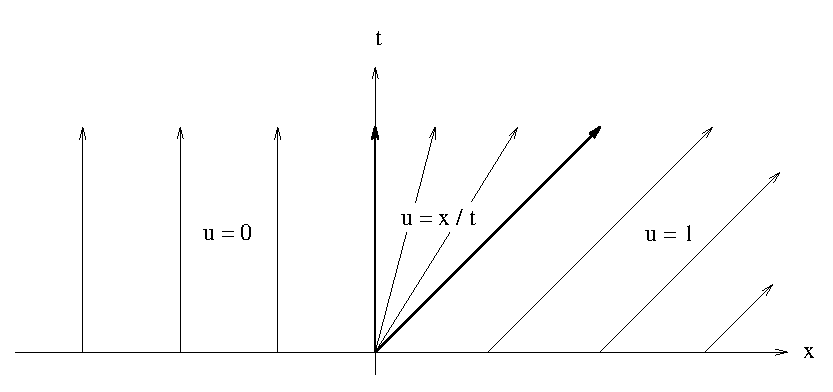
\includegraphics[height=3.3cm]{ambsthermopict/figRAchars.eps}
\caption{Characteristics of a rarefaction wave.}
\label{rarefactionfig}
\end{center}
\end{figure}
%\begin{figure}[bhpt]
%\begin{center}
%
\includegraphics[height=3.3cm]{figSHchars.eps}
%\caption{Characteristics of a shock}
%\label{shock}
%\end{center}
%\end{figure}






\section{Shock}

The solution with decreasing discontinuous initial data 
$u^0(x)=1$ for $x<0$, and $u^0(x)=0$ for
$x>0$, is a discontinuous \emph{shock wave} moving with speed $\frac{1}{2}$:
\begin{equation}\label{shock}
\begin{array}{rcl}
u(x,t)&=& 1 \quad\mbox{for}\quad x<\frac{t}{2},\\
u(x,t)&=& 0 \quad\mbox{for}\quad x>\frac{t}{2},  
\end{array}
\end{equation}
as shown in Fig \ref{shockfig}. We shall motivate that this is a 
\emph{physical shock}
satifying a 2nd Law.
\begin{figure}[bhpt]
\begin{center}
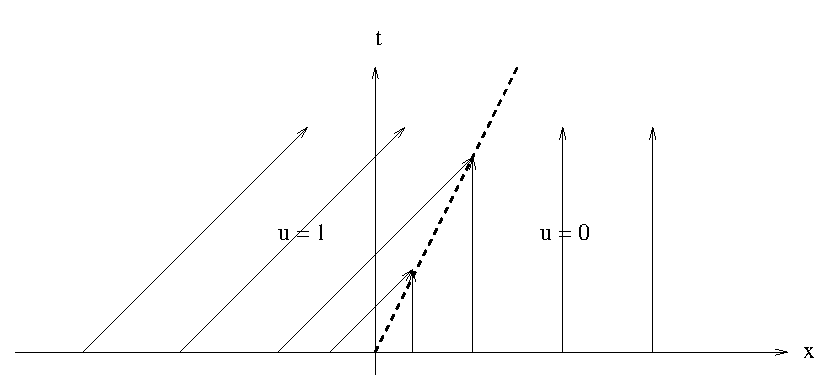
\includegraphics[height=3.3cm]{ambsthermopict/figSHchars.eps}
\caption{Characteristics of a shock}
\label{shockfig}
\end{center}
\end{figure}



\section{Weak solutions may be non-unique}

The rarefaction wave initial data 
$u^0(x)=0$ for $x<0$ and $u^0(x)=1$ for $x>0$, also admits
the alternative discontinuous weak solution 
\begin{equation}\label{unphyssol}
\begin{array}{rcl}
u(x,t)&=& 0 \quad\mbox{for}\quad x<\frac{t}{2},\\
u(x,t)&=& 1 \quad\mbox{for}\quad x>\frac{t}{2}, 
\end{array}
\end{equation}
corresponding to a discontinuity $\{x,t):x=st\}$ moving with speed
$s=\frac{1}{2}$. This solution is obviously
different from the rarefaction wave solution
(\ref{rarefaction}), which since it is a pointwise solution, also 
is a weak solution. Thus, we have in this case two different weak solutions, 
and thus we have an example of \emph{non-uniqueness of weak solutions.}
We shall see that the discontinuos solution (\ref{unphyssol}) 
violates the 2nd Law and thus is a \emph{non-physical shock solution}.
The physical solution in this case is the rarefaction wave
(which satisfies the 2nd Law with equality).



\section{The 2nd Law for Burgers Equation}

%The entropy inequalities are related to the Second Law of Thermodynamics
%stating that in a closed physical system, the entropy cannot
%decrease. Intuitively, the physical concept of ``entropy'' is related
%to ``disorder'' or ``loss of information'' and thus the  
%The Second Law states that disorder cannot decrease.
%To see how the Second Law in this form applies to the shock wave case above, 
%we note that the characteristics in this case ``converge into'' 
%the shock, which may be viewed as a ``loss of information'', or increase of entropy, 
%which is physically admissible.  On the other hand, for
%the unphysical solution (\ref{unphyssol}), the characteristics
%seem to ``emerge from'' the discontinuity, which may be viewed as
%some kind of ``creation of information'', which 
%would contradict the Second Law.
%Thus, in brief we may say that a discontinuous weak solution with
%the characteristics converging into the discontinuity, is a physical solution
%while it is unphysical if the characteristics are 
%divering out from the discontinuity.

We now check if (\ref{unphyssol}) satisfies the appropriate 
form of the 2nd Law (\ref{2ndlawBurgers})  
restricting space to $-1\le x\le 1$ and time to $0\le t\le 1$ assuming
the boundary conditions $u(-1,t)=0$ and $u(1,t)=1$. In this setting,
we obtain by multiplication of the viscous Burgers equation with $u$
and integrating by parts and using the sign of the viscous
term, the following form of the 2nd Law
\begin{equation}\label{2ndlawBurgers1}
-D_\nu (u;t)=  \dot K(u;t)+\int_{-1}^1(\frac{u^3}{3})^\prime =\dot K(u;t)+\frac{1}{3}
\end{equation} 
But for (\ref{unphyssol}) we have 
$\dot K=-\frac{1}{2}\frac{d}{dt}\frac{t}{2}=-\frac{1}{4}$, which
violates (\ref{2ndlawBurgers1}). 

Changing to the boundary conditions to $u(-1,t)=1$ and $u(1,t)=0$,
the 2nd Law changes to 
\begin{equation}\label{2ndlawBurgers2}
-D_\nu (u;t)= \dot K(u;t)+\int_{-1}^1(\frac{u^3}{3})^\prime =\dot K(u,t)-\frac{1}{3},
\end{equation} 
which is satisfied by (\ref{shock}) since now
$\dot K=\frac{1}{2}\frac{d}{dt}\frac{t}{2}=\frac{1}{4}<\frac{1}{3}$.

We conclude that a  discontinuous function $u(x,t)$ with the constant
states $u_-$ for $x<st$ and $u_+$ for $x>st$ corresponds
to a physical shock solution with shock speed $(u_-+u_+)/2$
if $u_-> u_+$, and to a non-physical 
shock if $u_-<u_+$.

We furher see that a shock dissipates substantial
kinetic energy into heat since for a viscous profile of width
$\nu$ joining two states $u_-$ and $u_+$   
\begin{equation}\label{Djump}
D_\nu (u;t)\equiv \int_\bbR\nu (u^\prime )^2\, dx\approx (u_--u_+)^2
\end{equation}
for small $\nu$.


\section{Burning Books}

The 2nd Law states that the characteristics of 
a physical shock  ``converge into'' the shock, corresponding
to $u_->u_+$. For the unphysical shock solutin
corresponding to the rarefaction
initial data with $u_-<u_+$, the characteristics
appear to ``emerge from'' the discontinuity. The
2nd Law thus allows information (features of the solution) to 
be ``destroyed'' (in a shock with converging characteristics), 
but not ``created out of nothing'' 
(in an unphysical rarefaction with diverging characteristics).
This connects to the essence of irreversibility: Burning books
can readily be done without any sophistication, while recovering the
original text from the ashes is impossible.  

\section{Stability of a Rarefaction Wave}

We shall now see that the 2nd Law can be replaced by a stability analysis
in its main mission to distingush physical shocks from unphysical shocks.
This reflects the fact that a stable process can be physically realized 
and observed, while an unstable process will have no permanence and
thus will be very difficult (or impossible) to realize.

The stability of a solution $u(x,t)$ is governed 
by the linearized equation 
\begin{equation}\label{linburgers}
\dot w+(uw)^\prime =0\quad\mbox{in }\bbR\times\bbR_+
\end{equation}
where $w$ represents a (small) perturbation (tending to zero for $\vert x\vert$
tending to infinity), and the solution $u$ acts as a 
given coefficient. The growth properties of the solution
$w$ of the linearized equation determines the stability:
If $w$ grows quickly in time, then the solution $u$ is unstable,
and if $w$ stays bounded, then $u$ is stable. Of course, stability
connects to finite precision: the level of the perturbation 
represents the precision.

We first consider the case of
a rarefaction wave given by (\ref{rarefaction}). Multiplying by $w$ and
integrating in space, we obtain by a simple computation using the fact
that $u^\prime (x,t)=1/t$ for $0\le x\le t$ and $u^\prime (x,t)=0$ else,
\[
\frac{d}{dt}\int_\bbR w^2(x,t)\, dx+
\int_0^t w^2(x,t)\frac{1}{t}\, dx =0,\quad\mbox{for }t>0,
\]
from which follows that
\begin{equation}\label{stabrarefaction}
\int_\bbR w^2(x,t)\, dx\le \int_\bbR w^2(x,0)\, dx\quad\mbox{for }t>0.
\end{equation}
This inequality shows that the $L_2$-norm in space
of a perturbation from initial data does not grow with time, 
which proves stability 
of a rarefaction wave. Note that this
argument builds on the fact that the rarefaction wave $u(x,t)$ is increasing in $x$ so that $u^\prime$ is
non-negative.

\section{Stability of Shock}

The stability proof used above to prove stability of a rarefaction
wave, does not work the same way for a shock, since in this case
$u(x,t)$ is decreasing with $x$. In fact a shock does not satisfy an
$L_2$ stability estimate of the form (\ref{stabrarefaction}). However,
one can prove instead an $L_1$-bound of the form
\begin{equation}\label{stabshock}
\int_\bbR \vert w(x,t)\vert\, dx\le \int_\bbR \vert w(x,0)\vert
\, dx\quad\mbox{for }t>0.
\end{equation}
This follows by multiplying (\ref{linburgers}) by $sgn (w)=+1$ if $w>0$ 
and $-1$ if $w<0$, to get by integration by parts:
\begin{equation}\label{linburgersL1}
\frac{d}{dt}
\int_\bbR\vert w(x,t)\vert\, dx +(u_--u_+)\vert w(\frac{t}{2},t)\vert =0,
\end{equation}
and using the fact that for a shock $u_+<u_-$.
Moreover, we will below with a different type of stability estimate
show that a shock is stable from computational RNS point of view, 
Thus, a shock is a stable phenomenon from both physical and computational
point of view.

%In one space dimension, shocks exist as piecewise constant
%(discontinuous) solutions, while in three space dimensions
%shocks in general generate turbulence. We present evidence in Vol 5.   

\section{Instability of Non-Physical Shock}

We saw above that the rarefaction wave solution is stable, and we now
study the stability of the alternative weak solution (\ref{unphyssol}).
By the same argument as used to prove (\ref{linburgersL1}) we obtain
\begin{equation}\label{linburgersL1unstable}
\frac{d}{dt}\int_\bbR\vert w(x,t)\vert\, dx =(u_+-u_-)\vert w(\frac{t}{2},t)\vert , 
\end{equation}
where now $u_+>u_-$. In this case, $\int_\bbR\vert w(x,t)\vert\, dx$
can grow arbitrarily fast, since the positive right hand side
in (\ref{linburgersL1unstable}) in no way can
be controled by the left hand side. We thus conclude that an 
unphysical shock is unstable.

\section{2nd Law $=$ Stability $+$ Finite Precision}
We thus have two methods
to single out physical shocks, one based on stability,
and the other based on the 2nd Law. This shows that ultimately the 2nd Law
expresses a stability condition, reflecting that Nature only can realize
phenomena which are properly stable, in its analog finite precision
computation. We thus may view the 2nd Law to express 
a combination of stability and finite precision.   


\section{A Traffic Model}

The equation (\ref{burgers}) with $f(u)=u(1-u)$ models the flow 
of cars along a highway represented by the $x$-axis with
$0\le u\le 1$ the car density and $0\le v=(1-u)\le 1$ the 
car velocity as a function of density: Sparse cars ($u\approx 0$)
move fast ($v\approx 1$) and packed cars ($u=1$) stand still
($v=0$). The equation (\ref{burgers}) then expresses
conservation of mass in the sense that there are no side roads
through which cars can enter or exit (and they cannot simply disappear
into the sky). 

We understand that if $u(x,t)$ is increasing
in $x$ so that the car density increases in the direction of motion,
then the car velocity will be decreasing in the direction of motion
which means that 
faster cars behind will approach slower cars ahead.
 But the $x$-axis
is a one-lane street and does not allow a faster car to overtake a slower
car, and so 
eventually faster cars will have to break in order to not run 
into slower cars ahead, that is, the law $v=(1-u)$ will have to
be violated and thus the conservation law (\ref{burgers})
cannot be satisfied pointwise. In the inviscid equation (\ref{burgers})
this will correspond to the appearence of a shock. The corresponding
regularized equation takes the form
\[
\dot u +((u(1-u))^\prime -\nu u^{\prime\prime} =0,
\]
which we formally can write as
\[
\dot u +(uv)^\prime =0
\]
with the modified velocity law
\[
v=(1-u-\frac{\nu}{u} u^\prime ),
\]
with the effect that in the dangerous case of 
increasing density ($u^\prime >0$),
faster cars will be slowed down more than slower cars and
collisions from behind will thus be avoided.

In this model the shock corresponds to the well-known situation 
when an inexperienced driver suddenly steps on the brake to avoid
collision into a cue, which in the regularized problem 
corresponds to the smoother action of an experienced driver
slowing down because the car density is larger
ahead than behind.





\section{Non-Existence Exact Euler Solutions}

We have seen that the inviscid Burgers equation has discontinuous
shock solutions, which can be viewed as weak solutions satisfying
a 2nd Law. One can thus speak about a shock solution as an exact 
weak solution of Burgers equation satisfying a 2nd Law, and 
this solution is the limit of regularized solutions as the 
viscosity tends to zero.
The goal of the classical mathematical analysis of conservation laws
based on regularization, is to establish a corresponding result for
the Euler equations: The goal is thus to prove the existence of a function
satisfying the Euler equations in a weak sense together with a 2nd Law,
as a limit of regularized solutions.

However, this goal has not been reached, and we have good reasons
to believe that it cannot be reached. This is 
because of the appearence of turbulent solutions to the 
regularized Euler equations which do not seem have a limit in the form
of a function. It is thus not meaningful to speak about 
exact solutions to the Euler equations, because such objects do not
exist, but we may speak about regularized solutions because
they do exist and we may view such solutions as approximate
solutions to the Euler equations.

With this perspective it is reasonable to view a shock solution
not as is usual as an exact weak solution to the Euler equations, 
but rather to view a viscous shock solution, an exact solution to the 
regularized Euler equations, as an approximate solution to the 
Euler equations. 
Thus only strong pointwise solutions could deserve the
title of ``exact solution''; a weak solution 
which is not a strong solution like a shock, could only be an approximate 
solution. This may seem to differ from the common way of looking at 
weak solutions of differential equations, as functions satisfying
the differential equation ``weakly exactly'', but this is not completely
natural since the notion of ``weakly'' has an element of ``inexactly''
built in. Only a strong pointwise solution can be an exact solution.
I somebody offers you to buy an unknown painting by
van Gogh,  which you are only allowed to inspect from a distance
of 10 meters, you may get suspicious and refrain from a deal.

 

\chapter{BurgersRNS}

\small
\begin{quote} But maybe that is our mistake: 
maybe there are no particle positions and velocities, but only waves. 
It is just that we try to fit the waves to our preconceived ideas of 
positions and velocities. The resulting mismatch is the cause of the 
apparent unpredictability. (Stephen Hawking 1988)
\end{quote}
\normalsize  

\section{Introduction}
We will now consider RNS applied to Burgers' equation as a simple
version of RNS. We recall that RNS is Galerkin's 
finite element method
combined with a weighted least-squares control of the
residual. RNS is based on  piecewise polynomial approximation
in space-time and offers spectrum of computational methods 
depending on the choice of the space-time
mesh, as presented in detail in \cite{cde,ambsflow}.
RNS uses piecewise polynomials which are
continuous in space and possibly discontinuous in time.
These variants are referred to as cG($p$)cG($q$) or cG($p$)dG($q$) with
cG($p$) referring to continuous piecewise approximation of degree $p$
in space, and cG($q$)/dG($q$) referring to  continuous/discontinuous
approxiamtion in time of degree $q$. RNS is \emph{Eulerian} if
the space-time mesh oriented along the space and time coordinate axis, 
is \emph{Lagrangean} if the space-time mesh is oriented along particle
paths in space-time, and \emph{Arbitrary Lagrangean-Eulerian} or \emph{ALE} 
if the space-time mesh is oriented according to some other feature such as
space-time gradients of the solution. 
Lagrangean variants are also referred to as \emph{characteristic Galerkin}, 
and Eulerian variants as \emph{streamline diffusion methods}.

In all these variants the space-time mesh is usually organized in
space-time slabs between discrete time levels, and RNS then
gives a time-stepping method allowing the solution to be
computed form one time level to the next progessing in time. The
space mesh may be changed across the discrete time levels to avoid 
mesh distortion and allow mesh adaption. In dG($q$) the
approximation is discontinuous in time and the space
mesh may vary from one slab to the next. If the space mesh is changed 
across a discrete time level in cG(q), then
a projection from the previous mesh 
to the new mesh is performed. The projection is built 
into the Galerkin method  through a jump term corresponding to a 
$L_2$ projection. The discrete solution between the
discrete time levels may be viewed as an approximate {\em transport} step,
and the whole process may be viewed as a method of the basic form
\emph{projection-transport}. 

The traditional finite difference methods are of Eulerian type with the 
first order Lax-Friedrichs' scheme from the 50s as a prototype on 
conservation form  
and with artificial viscosity proportional to the mesh size. The next 
generation
of classical schemes originates from Godunov's method in 1d, 
which is of the form projection-transport with piecewise constant 
(discontinuous) approximation  and a Riemann solver for the transport step. 
The multi-dimensional finite volume schemes 
developed in recent decades, use discontinuous polynomial
approximation with numerical fluxes often constructed using
1d Riemann solvers. 
All these methods may alternatively be viewed as particular 
RNS methods. 


%Galerkin/least squares methods were pionereed in the early
%1980s by Hughes followed by Johnson in the form of 
%streamline diffusion methods, see \cite{hughes}, \cite{johnson}, \cite{cime}.
 
\section{Semi-Discrete RNS for Burgers Equation}

For the purpose of analysis displaying essential aspects,
we consider a \emph{semi-discrete} RNS method for Burgers equation with
cG(1) discretization in space. Full discretization
with cG(q) or dG(q) in time can be analyzed similarly.
Let then for a
given mesh on $\bbR$ with 
mesh size $h$, $V_h$ be the set of continuous functions $v(x,t)$ 
which for $t\in I=[0,T]$ are piecewise linear in $x$ on the mesh.
The simplest version of semidiscrete RNS takes the form: 
Find $U\in V_h$ such that
\begin{equation}\label{RNSburgers} 
  ((R(U),v))+((hU^\prime ,v^\prime ))=0\quad\forall v\in V_h,
%+(\hat\epsilon \nabla U,\nabla v)_n
%  +([U_{n-1}],v_{n-1}^+)_\bbR =0,\quad\forall v\in V _n,
\end{equation}
where $R(U)=\dot U+UU^\prime$ is the Burgers residual, $((v,w))=\int_Q vw\, dxdt$ with $Q=\bbR\times I$ and $U(x,0)\in V_h$ 
interpolates $u^0(x)$. 
This is equivalent to a  system of ordinary differential equations
in time. We have here replaced residual stabilization by
$(hU^\prime ,v^\prime )$, and we thus consider 
a Galerkin method in space for a viscous Burgers equation
with viscosity $\nu =h$.    

%\[
%\delta =\frac{1}{2}(k_n^{-2}+h_n^{-2}A(U)^2)^{-1/2},
%\] 
%$\hat\epsilon =\max (\epsilon ,\gamma_1h^{2-\kappa}R(U),\gamma_2h^{\frac{3}{2}})$, and
%now $R(U)=\vert \dot U+A(U)U^\prime \vert + \vert [U_{n-1}]\vert/k_n$ on $S_n$. 
\section{Basic Energy Estimate as 2nd Law}

Choosing $v=U$ in (\ref{RNSburgers}), we obtain by 
integration by parts over $\bbR$ the following direct analog
of (\ref{2ndlawBurgers}):
\[
\dot K(U;t)=-D_h(U;t),\quad\mbox{for } t\in I.
\]
%
%\[
%K(U;t)=\frac{1}{2}\int_{\bbR} U^2(t)dt,
%\quad D_h(U;t)=\int_0^t\int_\bbR h(U^\prime )^2\, dxdt.
%\]
%This is the basic energy estimate for RNS for Burgers'equation,
%which is also a 2nd Law for the kinetic energy $K$.
In the presence of shocks, $D_h(U; t)$ will be substantial
and thus $U'$ will at shocks be large ($\sim h^{-1})$.



%\section{RNS and the 2nd Law}

%We shall now prove as a major observation of this note that
%RNS automatically satisfies the entropy inequality (\ref{entropyineq})
%in a weak sense, and thus automatically computes a physical solution
%without explicitely enforcing the entropy inequality. The key point is
%thus that construction of RNS as weak satisfaction of the conservation
%law combined with weighted least squares constrol of the pointwise
%residual, assures that a RNS solution also satisfies the entropy
%inequality characterizing physical solutions. In particular, there
%is no chance that RNS will produce an non-physical solution
%violating the entropy condition.

%To see this, we choose a smooth non-negative
%test function $\varphi$, write $w=\varphi  U$ and then choose
%in RNS the finite element test function $v=w_h$, where
%$w_h\in V_h$ is a nodal interpolant of $w$, noting that $w$ does
%not belong to $V_h$ in RNS in general. We then have with
%$\tilde U_n=\frac{1}{2}(U_n^++U_n^-)$, by integration by parts in space and time,
%\[ 
% -(\frac{1}{2}U^2,\dot\varphi )_{Q_N}
%-(\frac{1}{3}U^3,\varphi^\prime )_{Q_N}
%\]
%\[
%=\sum_{n=1}^N\bigl((R(U),w)_{S_n} +([U_{n-1}],
%\tilde U_{n-1}\varphi_{n-1}^+)_\bbR\bigr) 
%\]
%\[
%=\sum_{n=1}^N\bigl(R(U),\hat w_h)_{S_n}-(hR(U),\dot w_h+
%Uw_h^\prime )_{S_n}
%  +([U_{n-1}],\tilde U_{n-1}\varphi_{n-1}^+- w_{h,n-1}^+)_\bbR\bigr)
%\]
%\[
%\equiv I+II+III,
%\]
%where $\hat w_h=w-w_h$, and we used (\ref{RNSburgers}) with $v=w_h$.
%We now estimate the interpolation error $\hat w_h$ as follows:
%\[
%\Vert \hat w_h\Vert_{S_n}\le \Vert h^2D^2w\Vert_{S_n}\le Ch\Vert U\Vert_\infty ,
%\]
%where $D$ represents first order derivation in space or time,
%$C$ depends on first and second derivatives of $\varphi$
%and $\Vert U\Vert_\infty =\max_{Q_N}\vert U\vert\equiv M$. This type of estimate is 
%referred to as super-approximation since it contains the factor $h$ without paying the price 
%of first derivatives of $U$, which results from the special form of $w=\varphi U$ as a product
%of a finite element function $U$ and a smooth function. We conclude that
%\[
%I\le  CM\Vert hR(U)\Vert_{Q_N}\le CM\sqrt{h},
%\]
%where we used the basic energy estimate assuming $\Vert u^0\Vert\sim 1$. Further
%\[
%II=\sum_{n=1}^N(hR(U),\frac{\partial}{\partial t} \hat w_h+
%U\hat w_h^\prime )_{S_n}-\sum_{n=1}^N(hR(U),\dot w+
%Uw^\prime )_{S_n}=II_a+II_b.
%\]
%We have again by super-approximation and the energy estimate that
%$II_a\le CM\sqrt{h}$, and 
%\[
%II_b = -\sum_{n=1}^N(hR(U),\dot U\varphi +
%UU^\prime\varphi )_{S_n}-\sum_{n=1}^N(hR(U),U\dot\varphi +
%UU\varphi^\prime )_{S_n}
%\]
%\[
%\le -\sum_{n=1}^N(hR(U),R(U)\varphi )_{S_n}+CM\sqrt{h}\le CM\sqrt{h},
%\]
%where we used the non-negativity of $\varphi$. The term $III$
%is estimated similarly. We conclude that for all non-negative
%test functions $\varphi$, we have
%\[ 
% -(\frac{1}{2}U^2,\dot\varphi )_{Q_N}
%-(\frac{1}{3}U^3,\varphi^\prime )_{Q_N}\le CM\sqrt{h},
%\] 
%where $M$ is a bound for $U$ and $C$ depends on up to second derivatives
%of $\varphi$. This expresses that the RNS solution $U$
%approximately satisfies the entropy inequality in weak form
%and the approximation improves as $h$ gets smaller. We refer to this property of RNS
%as entropy consistency. In particular
%RNS cannot compute a non-physical solution significantly
%violating the entropy inequality significantly. Note that the $M$-bound on $U$ is natural
%and can be proved by a maximum principle if RNS is suitably modified.  

%We have now established the key feature of RNS to automatically satisfy
%the entropy inequality approximately, as a consequence of the
%least squares stabilization. The key to the proof is the super-approximation
%making it effectively possible to choose $U\phi$ as a test function in RNS, 
%from which entropy consistency follows using the positivity of the least squares
%term, which reflects that
%the entropy inequality is obtained by multiplication of the viscid Burgers' equation
%by $\eta^\prime (u)\varphi =u\varphi$. Note that choosing $U$ as a test function 
%gives the basic energy estimate, which is the integrated form of the entropy
%inequality, and the step to choose instead $(U\phi )_h$ is not 
%large, but requires the least squares stabilization to work out





\section{A Posteriori Error Estimation by Duality}

We shall now prove we the following a posteriori 
error estimate, where $u$ is the solution of the viscous Burgers equation 
with $\nu =h$:
\begin{equation}\label{apostburgers}
\Vert u-U\Vert_{Q}\le S\Vert hR(U)\Vert_{Q},
\end{equation}
where $\Vert\cdot\Vert_Q$ is the $L_2(Q)$-norm and 
\begin{equation}\label{stabburgers}
S=\frac{\Vert h\phi^{\prime\prime}\Vert_{Q}
}{\Vert e\Vert_{Q}},
\end{equation}
is a stability factor defined by the solution 
$\varphi$ of the following 
linearized dual problem:
\begin{equation}\label{burgdual}
\begin{array}{rcl}
 -\dot\varphi - 
a\varphi^\prime -
h\varphi^{\prime\prime}  =  e, & & \mbox{in }Q,\\
\varphi (x,t)  \rightarrow  0, & & x\rightarrow \pm\infty ,t\in I , \\
\varphi (x,T)  =  0,  & & x\in \bbR ,
\end{array}
\end{equation}
{\flushleft where} $a=(u + U)/2$. We notice that the dual problem
has a viscous term with viscsoity coefficient $h$.



To prove the a posteriori error estimate (\ref{apostburgers})
we multiply (\ref{burgdual}) by $u-U$ and integrate in space and time
to get the error representation
\[
\Vert u-U\Vert_{Q}^2=((R(U),\phi ))+((hU^\prime ,\varphi^\prime )).
\]
We then use the Galerkin orthogonality (\ref{RNSburgers})
with $v=\Phi\in V_h$ an interpolant of the dual solution $\varphi$, to get
\[
\Vert u-U\Vert_{Q}^2=((R(U),\phi -\Phi ))+
((hU^\prime ,\varphi^\prime -\Phi^\prime )),
\]
which combined with an interpolation error bound of the form 
\[
\Vert\varphi -\Phi\Vert_{Q}+\Vert h(\varphi^\prime -\Phi^\prime )\Vert_{Q}\le
C_i\Vert h^2\varphi^{\prime\prime}\Vert_{Q},
\]
where $C_i$ is an interpolation constant, shows that
\[ 
\Vert u-U\Vert_{Q}^2\le C_i\Vert hR(U)\Vert_{Q}\Vert h\varphi^{\prime\prime}\Vert_{Q},
\]
where $R(U)$ has been augmented by the contribution $\Vert hU^\prime\Vert_Q$,
which proves (\ref{apostburgers}), setting $C_i=1$ for simplicity.

By the basic energy stability estimate, we have
\[
\Vert hU^\prime\Vert_{Q}\le\sqrt{h}\quad \mbox{if }\Vert u^0\Vert_\bbR =1,
\]
suggesting the same estimate for $\Vert hR(U)\Vert_Q$, 
which of course is checked a posteriori, and thus we expect
\begin{equation}\label{apostburgers2}
\Vert u-U\Vert_{Q}\le S\sqrt{h} .
\end{equation}
We shall now prove that for a shock $S\sim 1$, which shows that
a shock is computable with RNS, with a $L_2(Q)$ error of size $\sqrt{h}$, which
is optimal from approximation point of view (if we consider 
the exact solution $u$ to be discontinuous) 
and $U$ is continuous in $x$ on the mesh.


\section{Stability Estimate for a Shock}

We shall now investigate the stability properties of the dual problem
(\ref{burgdual}) and seek to bound 
$h\phi^{\prime\prime}$ in terms of the right hand side
$e$. For simplicity we linearize at the exact solution 
$u(x,t)$ (instead of the mean value
$(u+U)/2$) and thus consider the dual problem
\begin{equation}\label{burgdual1}
\begin{array}{rcl}
 -\dot\phi - 
u\phi^\prime -
h\phi^{\prime\prime}  =  e, & & \mbox{in } Q,\\
%\phi (x,t)  \rightarrow  0, & & x\rightarrow \pm\infty ,  \\
\phi (\cdot ,T)  =  0.
\end{array}
\end{equation}
The stability properties are largely determined by the sign of $u^\prime$,
which reflects the change of the direction $u$ of the characteristics. If
$u^\prime \le 0$, then the characteristics converge with increasing $t$,
which typically occurs in the case of a shock. If $u^\prime \ge 0$,
then the characteristics diverge, which typically occurs in the
case of a rarefaction. If $u^\prime $ is bounded below by a moderate
constant, e.g. $u^\prime\ge 0 $,  then we may
estimate $\Vert \phi\Vert_{L_\infty (L_2(\bbR ))}$ and
$\Vert\sqrt{h}\phi^\prime\Vert_Q$  in terms of a moderate constant
times $\Vert e\Vert_{Q}$, which we refer to as 
{\it weak stability}. 
If $u^\prime$ is bounded above by a moderate constant, 
e.g. $u^\prime\le 0$, 
then we may estimate $\Vert h\phi^{\prime\prime}\Vert_{Q}$ in terms of
a moderate constant times $\Vert e\Vert_{Q}$, which we refer to as {\it strong stability},
because we estimate second derivatives of $\phi$, cf. (\ref{stabburgers}). 
These estimates are proved by multiplying by $\phi$ and 
$-h\phi^{\prime\prime}$, respectively,
bringing in the positive stabilizing terms 
$\frac{1}{2}u^\prime \phi^2$ and $-\frac{1}{2}h u^\prime (\phi^\prime )^2$,
respectively.

We now give the details in the case of a shock with $u^\prime\le 0$, where
we assume $u$ is differentiable with a very large negative $x$-derivative
close to the shock.  We indicate the general nature of the characteristics of the dual problem 
in Fig \ref{chardualshock}.  
We shall prove that the solution $\phi$ of (\ref{burgdual1}) satisfies
\begin{equation}\label{strongstabest}
\Vert{h}\phi^{\prime\prime}\Vert_{Q}+
\Vert\dot\phi+u\phi^\prime\Vert_{Q}
+\sup_{0<t<T}\Vert{h}^{1/2}
\phi^\prime (\cdot , t)\Vert_{R}
\leq 3\Vert e\Vert_{Q}.
\end{equation}
To see this we multiply the first equation in (\ref{burgdual1}) by
$-h\phi^{\prime\prime}$, integrating by parts with respect to $x$, 
and integrating in time over $(\tau ,T)$ with $0<\tau <T$,
we get with $Q_{\tau} =\bbR\times (\tau ,T)$
\begin{equation}\begin{array}{l}
\frac{1}{2}\int_{\bbR}h\left(
\phi^\prime (\cdot ,\tau )\right)^2 dx 
+\int_{Q_{\tau}}\left(h\phi^{\prime\prime}\right)^2\,dxdt +\int_{Q_{\tau}}\frac{1}{2}
\left(uh\left(\phi^\prime\right)^2\right)^\prime ~dxdt  \vspace{4mm} \\
 \leq \frac{1}{2}\int_{Q_{\tau}}\left({h}u^\prime
\left(\phi^{\prime}\right)^2+e^2+\left(h\phi^{\prime\prime}\right)^2\right)~\mbox{d}x\mbox{d}t,
\end{array}
\end{equation}
which proves the desired result stating that $S\sim 1$ for a shock.

\begin{figure}[ht]\label{chardualshock}
\centerline{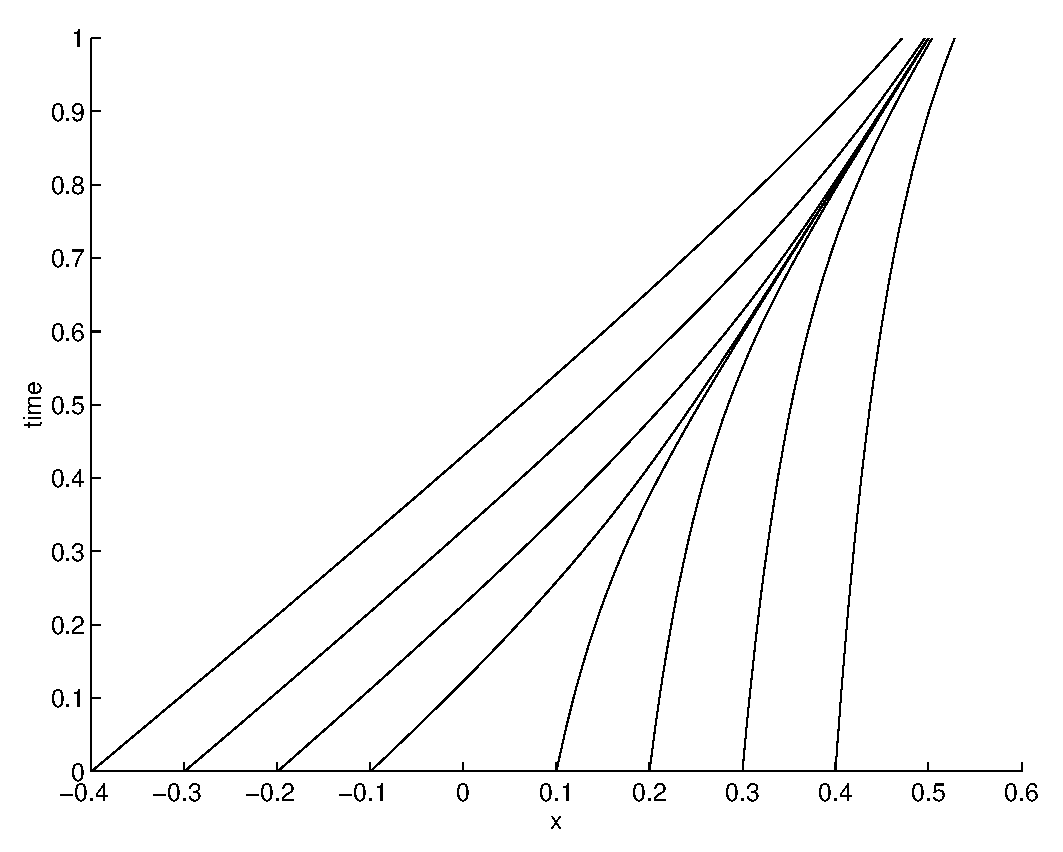
\psfig{figure=ambsthermopict/figCHARS.eps,height=2.5in,width=4in}}
\caption{Characteristics of the dual problem for a 
regularized shock solution.}
\end{figure}


As comparison, let us now attempt to derive a weak stability  estimate 
for (\ref{burgdual1}) in the case $u$ is a shock.
Multiplication 
by $\phi$ and integration over $Q_\tau$ gives
\[
\begin{array}{l}
 \frac{1}{2}\int_R
\phi^2(x,\tau )~dx + h\int_{Q_\tau}\left(
\phi^\prime (x,t)\right)^2~dxdt \vspace{3mm}\\
= -\frac{1}{2}\int_{Q_\tau}u^\prime 
\phi^2(x,t)~dx +\int_{R}e(x,t) \phi(x,t)~dx .
\end{array}\]
Since $u^\prime$ is large negative in the case of a shock, we have
large positive term of the right hand side, and using a Gronwall
inequality would results in a very large stability
factor. On the other hand, we show below weak stability for a 
rarefaction wave with $u^\prime\ge 0$, reflecting the 
above stability result for the perturbation equation.



Summing up, we see that for a shock, the linearized dual problem statisfies a strong
stability estimate with a stability factor of moderat size, while
a corresponding weak stability estimate appears to have a very large
stability factor. These stability features may be understood in a qualitative
sense, by pondering the directionality of the characteristics and the nature
of the $L_2$-norm. 

\section{Stability Estimates for a Rarefaction Wave}

We now consider the linearized dual Burgers' equation (\ref{burgdual1}),
linearized at the exact solution $u(x,t)=x/t$, corresponding to a rarefaction wave. 
Multiplying now (\ref{burgdual1}) by 
$-ht\phi^{\prime\prime}$, and using standard manipulations,
we obtain the following weighted norm strong stability estimate for $0<\tau <T$,
\begin{equation}\label{weightedstrongstab}
\Vert\tau^{1/2}h^{1/2}\phi^\prime\Vert 
+\Vert \omega h\phi^{\prime\prime}\Vert_{Q_\tau }
\leq \Vert \omega e\Vert_{Q_\tau } ,
\end{equation}
where $\omega (t)=t^{1/2}$ acts as a weight. 

A weighted norm analog of the a posteriori error estimate (\ref{apostburgers}) takes the form
\begin{equation}\label{weightedapostburger}
\Vert \omega^{-1} e\Vert_{Q_N}\le S_\omega\Vert \omega^{-1} hR(U)\Vert_{Q_N}
\end{equation}
with $S_\omega$ defined by the direct weighted norm analog of (\ref{stabburgers}).
The estimate (\ref{weightedstrongstab}) then shows that $S_\omega \sim 1$, 
and thus a rarefaction wave solution is computable in the weighted
norm with computational work corresponding to interpolation.
Note that the presence of the weight $t^{-1/2}$ will force more
stringent demands on the mesh for $t$ close to zero, which will
force an accurate resolution of the initial phase of the rarefaction.
This is intuitively reasonable and corresponds to the fact that an initial
error in the computation of a rarefaction will get amplified as time goes,
because characteristics diverge forward in time. On the other hand,
in the case of a shock, an initial error may be eliminated at later times,
because of converging characteristics, Thus, a rarefaction is more delicate
to compute than a shock, which we will see in the computational results 
we now present.





\section{Dual Solution and Stability Factors}

We display below RNS computations of a combination of  
a rarefaction wave and a shock using the cG(1)dG(0)-
method on a uniform space mesh with $h=10^{-3}$
and time step $10^{-4}$ taken from \cite{burman}.  We plot 
the computed solution at t=0,  t=0.3 , t=0.8, t=1 in Fig \ref{shockrarefaction}.
We see that the initial discontinuity
develops into a rarefaction and that a shock is formed for $t\approx 0.5$.

\begin{figure}[bhpt]
%\begin{center}

\includegraphics[height=4cm]{initburger}

\includegraphics[height=4cm]{03Tburger}

\includegraphics[height=4cm]{08Tburger}

\includegraphics[height=4cm]{Tburger}
\caption{A combined rarefaction and shock wave}
\label{shockrarefaction}
%\end{center}
\end{figure}


We solve the dual problem
using the following different approximations of the coefficient $a=(u+U)/2$
and the error $e$, with $\bar u$ the analytical, inviscid solution, 
and $U(h)$ the finite element solution on a mesh of size $h$:
(i) $a=(\bar u+U(h))$ and $e=\bar u-U(h)$,
(ii) $a=U(h)$ and $e=\bar u-U(h)$, (iii) $a=(U(h/4)+U(h))/2$ and $e=U(h/4)-U(h)$. 
We plot the corresponding dual solutions $\phi$ 
at the same time levels as above, but in revers
e order (t=1, t=0.8, t=0.3 , t=0)
in Fig \ref{dualsolution}.
\begin{figure}[bhpt]\label{dualsolution}
%\begin{center}

\includegraphics[height=4cm]{bdual10}

\includegraphics[height=4cm]{bdual08}

\includegraphics[height=4cm]{bdual03}

\includegraphics[height=4cm]{bdual00}
\caption{Dual solution in reverse time.}
%\end{center}
\end{figure}
We also plot in Fig. \ref{dualsol2} the corresponding second 
derivatives $\phi^{\prime\prime}$. 
\begin{figure}[bhpt]
%\begin{center}

\includegraphics[height=4cm]{bdualxx10}

\includegraphics[height=4cm]{bdualxx08}

\includegraphics[height=4cm]{bdualxx03}

\includegraphics[height=4cm]{bdualxx00}
\caption{Second deriatives of the dual solution in reverse time}
\label{dualsol2}
%\end{center}
\end{figure}
We note the change of $\vert\phi^{\prime\prime}\vert$, which may be viewed as a weight
in the a posteriori error estimate, from being 
large close to the shock at final time towards being large 
close to the initial discontinuity at $(x,t)=(0.2,0)$ initiating the rarefaction.
We see that that it is the data from the rarefaction at final time which
generates the large values of $\phi^{\prime\prime}$ at $t=0$, and not those
from the shock. This indicates that a rarefaction is more delicate to compute than a shock. 


We plot in Fig. \ref{stabfactorstrong} the strong stability factor $S$ defined
by (\ref{stabburgers})
for (i)-(iii) and $h=0.0001, \,h=0.00005, \,h=0.00001$.
\begin{figure}
%\begin{center}

\includegraphics[height=6cm]{S2veps}
\caption{Strong stability factor for different $h$}
\label{stabfactorstrong}
%\end{center}
\end{figure}
We see that $S\sim 1$, which shows that the Burgers' solution 
consisting of a rarefaction and shock wave is computable in 
$L_2(Q_N)$ with work comparable to interpolation.



\iffalse  % --- removed: placeholder section with missing figures (sphere/cylinder eps files not in repo) ---
\section{Turbulent Bluff Body Flow}
We show RNS flow with shocks around a sphere and cylinder in
Figs. \ref{sphere} and \ref{cyl}. This section will be
extended with turbulent/shock flow around a cube and sphere.
\begin{figure}[bhpt] 
\centerline{ 
\includegraphics[height=5.5cm]
{eps/3Dden.eps} 
\includegraphics[height=5.5cm]
{eps/3D_den_mach.eps} 
} 
\caption{Flow around a sphere}
\label{sphere} 
\end{figure}
\begin{figure}[bhpt] 
\centerline{ 
\includegraphics[height=10cm]
{eps/sphere_mesh.eps} 
} 
\caption{Mesh around a sphere}
\label{spheremesh} 
\end{figure}
\begin{figure}[bhpt] 
\centerline{ 
\includegraphics[height=5.5cm]
{eps/velocity_con.eps} 
\includegraphics[height=5.5cm]
{eps/velocity_con_2.eps}
} 
\caption{Section of 2d flow around a cylinder}
\label{cyl} 
\end{figure}

\section{Turbulent Flow in Heat Engines and Refrigerators}
This section will contain RNS simulations of diffuser flow with
gas expanding under cooling while getting heated by turbulence,
with the objective of computing losses and efficiency.
\fi  % --- end removed placeholder block (Bluff Body + Heat Engines stubs) ---

%\section{Transonic Flight}

%\section{Supersonic Flight}















\begin{thebibliography}{9}

\bibitem{RealQM2026} C.~Johnson, \emph{Real Quantum Mechanics: A
Multiphase 3D Continuum Formulation Realised through Mind--AI
Cooperation}, Applied Mathematics Body and Soul, Vol.~VI, 2026.

\bibitem{FEniCS2012} A.~Logg, K.-A.~Mardal and G.~N.~Wells (eds.),
\emph{Automated Solution of Differential Equations by the Finite Element
Method: The FEniCS Book}, Lecture Notes in Computational Science and
Engineering, Vol.~84, Springer, 2012.

\bibitem{Davis2000} M.~Davis, \emph{The Universal Computer: The Road
from Leibniz to Turing}, W.~W.~Norton, New York, 2000.

\bibitem{bergmann} P.~Bergmann, \emph{Basic Theories of Physics},
Prentice-Hall, 1950.

\bibitem{bodysoul} http://www.bodysoulmath.org.

\bibitem{burman} E.~Burman, Adaptive finite element methods
for compressible two-phase flow, Ph D Thesis, Chalmers University of Technology,
1998.

\bibitem{boltzmann}L.~Boltzmann, \emph{Lectures on Gas Theory}, Dover, 1964.

\bibitem{brush1} Stephen Brush, \emph{The Kind of Motion We Call Heat: Physics
and the Atomists}, Elsevier Science, 1986.

\bibitem{brush2} S. Brush, \emph{The Kind of Motion we call Heat. 
A History of the Kinetic Theories of Gases in the 19th century}, 
Volumes I and II, Studies in Statistical Mechanics, Vol. VI, 
E.W. Montroll and J.L. Lebowitz (eds.), North-Holland 
Publishing Company, Oxford, 1976.

\bibitem{carnot} Sadi Carnot, in Reflections of the motive power of fire and 
on machines fitted to develop that power, 1824.

\bibitem{clausius1} Rudolph Clausius, \emph{Abhandlungen \"uber die
Mechanische W\"aremtheorie}, Band 1-2, 1864.

\bibitem{clausius2} R. Clausius, 
\"Uber die W\"armeleitung gasf\"ormiger K\"orper, 
Annalen der Physik 125: 353-400, 1865.


\bibitem{davies} Paul Davies, \emph{The Cosmic Blueprint,
New Discoveries in Nature's Creative Ability to Order the Universe},
Templeton Foundation Press.

\bibitem{cde} K.~Eriksson, D.~Estep and C.~Johnson, \emph{Computational
Differential Equations}, Cambridge University Press, 1996. 


\bibitem{euler} L.~Euler, Principes g\'en\'eraux du mouvement des fluides 
(General laws of the motion of fluids), Archives of the French Academy 
of Sciences, 1755.

\bibitem{feynman} Richard Feynman, \emph{The Feynman Lectures on Physics},
Caltech, 1963.

\bibitem{fenics} The FEniCS Project, http://www.fenics.org.

\bibitem{foucault} Michel Foucault, Discipline and Punishment, The Birth
of the Prison, Vintage books, 1991.

\bibitem{guillemin} V.~Guillemin, \emph{The Story of Quantum Mechanics}, 
Scribner, 1968.


\bibitem{hoffman}J.~Hoffman, A general Galerkin finite element
method for turbulent compressible flow, Finite Element Center
Preprint 2006-13.

\bibitem{dreams}J.~Hoffman, C.~Johnson and A.~Logg, 
\emph{Dreams of Calculus: Perspectives on Mathematics Education}, Springer, 2006. 

\bibitem{jfm}J.~Hoffman and C.~Johnson, 
Finally, Resolution of d'Alembert's Paradox, to appear in  
Journal of Mathematical Fluid Mechanics, 2008.


\bibitem{ambsflow}J.~Hoffman and C.~Johnson, 
\emph{Computational Turbulent Incompressible Flow}, Applied Mathematics
Body and Soul Vol 4, Springer, 2007.


\bibitem{compquantum} J.~Hoffman and C.~Johnson
\emph{Computational Quantum Mechanics}, to appear.

\bibitem{cime} C.~Johnson, Adaptive finite element methods for conservation
laws, Advanced Numerical Approximation of Nonlinear Hyperbolic Equations,
Springer Lecture Notes in Mathematics 1697 (1998), 269-323.

\bibitem{arrow} C. Johnson, \emph{The Clock 
and the Arrow: A Brief Theory of Time}, Computational Technology
Laboratory Preprint, 2008.


\bibitem{blackbody} C. Johnson, \emph{Computational Black-Body
Radiation},  Computational Technology
Laboratory Preprint, 2008.

\bibitem{kelvin}
W.~Thomson (Lord Kelvin), On the dynamical theory of heat; with numerical 
results deduced from Mr. Joule's equivalent of a thermal unit and M. 
Regnault's observations on steam, Math. and Phys. Papers vol.1, p 179, 1851.

\bibitem{laughlin} Robert Laughlin, \emph{A Different Universe}, 2005.

\bibitem{lieb} Elliot Lieb and Jakob Yngvason, The Physics and Mathematics
of the Second Law of Thermodynamics, Physics Reports 310, 1-96 (1999).



\bibitem{leff} Leff, H.S. and Rex, A.F. (eds),
Maxwell's Demon: Entropy, Information, Computing. 
Bristol: Adam-Hilger, 1990. 

\bibitem{foundphysics} Lindsay and Margenau, \emph{Foundations of Physics},
1936.

\bibitem{kuhn1} Thomas Kuhn, \emph{Black-Body Theory and the 
Quantum Discontinuity},
1894-1912, Oxford Univ Press 1978.

\bibitem{laurendau} M.~Laurendau, \emph{Statistical Thermodynamics, Fundamentals
and Applications}, Cambridge University Press, 2005.

\bibitem{feireisl} Measure-vaued solutions to the complete Euler system revisited, Zeitschrift f\"ur angewandte Mathematik und Physik, June 2018. 69:57.
\bibitem{chenwang} The Cauchy Problem for the Euler Equations Compressible Fluids, Handbook of Mathematical Fluid Dynamics (eds S.J Friedlander and D. Serre), Volume I, Chapter 5, Elsevier 2012.

\bibitem{serre} Handbook of Mathematical Fluid Dynamics Vol I and II, S.J. Friedlander and D. Serre (eds), Elsevier 2002.

\bibitem{dafermos} C.M Dafermos, Maximal dissipation in equations of evolution, J. Differential Equations 252, 2012, 567-587.






%\bibitem{tegmark} Max Tegmark,
%The Interpretation of Quantum Mechanics: Many Worlds or Many Words?,
%in Fundamental Problems in Quantum Theory, eds. Rubin and Shih.

\bibitem{lieb} E. Lieb and J. Yngavason, The Physics and Mathematics of the Second Law of Thermodynamics, 1997.



\bibitem{loschmidt} J. Loschmidt, Sitzungsber. Kais. Akad. Wiss. Wien, Math. 
Naturwiss. Classe 73, 128-142, (1876).


\bibitem{ockham} William Ockham (1285-1349):
``Entia non sunt multiplicanda praeter necessitatem''
(Entities should not be multiplied unnecessarily). 

\bibitem{planck1} Max Planck, \"Uber den zweiten Hauptsatz der mechanischen 
W\"armetheorie, Dissertation, Berlin, 1879.

\bibitem{planck2} Max Planck, \emph{Vorlesungen \"uber Thermodynamik}, 1897.

\bibitem{planck3}
Max Planck,  Acht Vorlesungen \"uber Theoretische Physik, F\"unfte Vorlesung:
W\"armestrahlung und Elektrodynamische Theorie, Leipzig, 1910.



%\bibitem{planck4} ...Mechanically, the task seems impossible, and we will just
%have to get used to it (quanta) (Planck 1909).



 






\bibitem{popper} Karl Popper, The Logic of Scientific Discovery, 1949.
 
\bibitem{schrodinger2} E.~Schr\"odinger, 
\emph{The Interpretation of Quantum Physics}, 
Ox Bow Press, Woodbridge, CN, 1995.

\bibitem{shannon} C. E. Shannon, A mathematical theory of communication,
The Bell System Technical Journal, Vol. 27, pp 379-423, 623-656, July, Oct,
1948.

\bibitem{truesdell} C.~Truesdell, \emph{The Tragicomial History of 
Thermodynamics
1822-54}, Springer, 1980.

\bibitem{tegmark} Max Tegmark,
The Interpretation of Quantum Mechanics: Many Worlds or Many Words?,
in Fundamental Problems in Quantum Theory, eds. Rubin and Shih.

\bibitem{uffink} J.~Uffink, Bluff your way in the Second Law of Thermodynamics,
Department of History and Foundation of Science, University of Utrecht, 2001.

\bibitem{zeh} H.D. Zeh, in The problem
of conscious observation in quantum mechanical description,
ArXiv Quant-Phy June 2000.  

%\bibitem{planck3}
%Either the quantum of action was a fictional quantity,
%then the whole deduction of the radiation law was essentially an
%illusion representing only an empty play on formulas of no significance,
%or the derivation of the radiation law was based on sound physical conception.
%(Planck)

%\bibitem{planck4} ...Mechanically, the task seems impossible, and we will just
%have to get used to it (quanta) (Planck 1909).







 



%\bibitem{born2} Schr\"odinger was, to say the least, as stubborn as Einstein
%in his conservative attitude towards quantum mechanics; indeed, he not only
%rejected the statitical interpretation but insisted that his wave mechanics
%meant a return to a classical way of thinking. He would not accept
%any objection to it, not even the most weighty one, which is that
%a wave in $3n$-dimensional space, such as needed to describe the 
%$n$, is not a classical concept and cannot be visualized. 
%(Born in the Born-Einstein Letters)



%\bibitem{born3} ``De Broglie, the creator of wave mechanics, accepted
%the results of quantum mechanics just as Schr\"odinger did, but not
%the statistical interpretation.'' (Born in the Born-Einstein Letters)

%\bibitem{born4} ``I cannot understand how you can combine an entirely
%mechanistic universe with the freedom of the ethical will''. (Born in the
%Born-Einstein Letters)  











\end{thebibliography}

    



 









